% shtthesis, an unofficial LaTeX thesis template for ShanghaiTech University.
% Copyright (C) 2022 Li Rundong <rundong.001@gmail.com>
%
% This program is free software: you can redistribute it and/or modify
% it under the terms of the GNU General Public License as published by
% the Free Software Foundation, either version 3 of the License, or
% (at your option) any later version.
%
% This program is distributed in the hope that it will be useful,
% but WITHOUT ANY WARRANTY; without even the implied warranty of
% MERCHANTABILITY or FITNESS FOR A PARTICULAR PURPOSE.  See the
% GNU General Public License for more details.
%
% You should have received a copy of the GNU General Public License
% along with this program.  If not, see <https://www.gnu.org/licenses/>

% graduate setup
% \documentclass[master, anonymous]{shtthesis}
\documentclass[master]{shtthesis}
\shtsetup{
  degree-name = {工学硕士},
  degree-name* = {Master~of~Science~in~Engineering},
  % secret-level = {白给},
  title = {三维环境中人和物体单目重建},
  title* = {3D Monocular Human-Object Reconstruction},
  keywords = {人-物交互,空间关系,单目重建,归一化流,三视视觉},
  keywords* = {Human-Object Interaction, Spatial Relation, Monocular Reconstruction, Normalizing Flow, 3D Vision},
  author = {霍超凡},
  author* = {Huo~Chaofan},
  institution = {上海科技大学信息科学与技术学院},
  institution* = {School~of~Information~Science~and~Technology\\%
                  ShanghaiTech~University},
  supervisor = {汪婧雅~助理教授},
  supervisor* = {Professor~Wang~Jingya},
  supervisor-institution = {上海科技大学信息科学与技术学院},
  discipline-level-1 = {计算机科学与技术},
  discipline-level-1* = {Computer~Science~and~Technology},
  bib-resource = {Biblio/ref.bib},
}

% `latex' and `shell' environments are adapted from `thuthesis'
\usepackage{listings}
\usepackage{amsthm}
\usepackage{multirow}
\usepackage{multicol}
\usepackage{pifont}
\usepackage{bm}
\usepackage{color}
\usepackage{booktabs}
\usepackage{bbding}
\usepackage{algorithm}  
\usepackage{algorithmicx} %或者\usepackage{algorithmic}
\usepackage{algpseudocode}
\newcommand\prompt{\textup{\$}}
\lstdefinestyle{lstStyleBase}{%
  basicstyle=\small\ttfamily,
  aboveskip=\medskipamount,
  belowskip=\medskipamount,
  lineskip=0pt,
  boxpos=c,
  showlines=false,
  extendedchars=true,
  upquote=true,
  tabsize=2,
  showtabs=false,
  showspaces=false,
  showstringspaces=false,
  numbers=none,
  linewidth=\linewidth,
  xleftmargin=4pt,
  xrightmargin=0pt,
  resetmargins=false,
  breaklines=true,
  breakatwhitespace=false,
  breakindent=0pt,
  breakautoindent=true,
  columns=flexible,
  keepspaces=true,
  gobble=0,
  framesep=3pt,
  rulesep=1pt,
  framerule=1pt,
  frame=l,
  rulecolor=\color{ShtRed},
  backgroundcolor=\color{gray!5},
  stringstyle=\color{green!40!black!100},
  keywordstyle=\bfseries\color{blue!50!black},
  commentstyle=\slshape\color{black!60},
  escapeinside={`'},
}
\lstdefinestyle{lstStyleShell}{%
  style=lstStyleBase,
  language=bash}
\lstdefinestyle{lstStyleLaTeX}{%
  style=lstStyleBase,
  language=[LaTeX]TeX}
\lstnewenvironment{latex}{\lstset{style=lstStyleLaTeX}}{}
\lstnewenvironment{shell}{\lstset{style=lstStyleShell}}{}

\usepackage{hologo}
\ifluahbtex
  \usepackage{emoji}
\else
  \providecommand{\emoji}[1]{ \fbox{\emph{#1}} }
\fi

\usepackage{subcaption}
\usepackage{ctable}
\usepackage[list=off]{bicaption}
\captionsetup[figure][bi-second]{name=Figure}
\captionsetup[table][bi-second]{name=Table}

\makeatletter
  \def\ifundergraduate{\ifsht@undergraduate}
  \def\ifgraduate{\ifsht@graduate}
\makeatother

\begin{document}

\maketitle

\frontmatter
\begin{abstract}[flattitle]
单目人和物体交互的三维重建任务是指从单视角的图片中重建出人和物体的三维信息,是计算机视觉和计算机图形学交叉领域的一个重要研究方向,在增强现实、物体操控学习、动画电影制作、机器人模仿学习、人体行为理解和具身智能等领域存在重要的应用。然而现存技术存在重建速度慢、对域外物体泛化能力弱、严重依赖三维标签监督等缺点,阻碍了其在实际场景中的应用。为了解决这些问题,本文围绕单目人和物体联合重建这个主题,在人和物体三维空间关系建模和预测、同类别物体的域外泛化、二维信息监督下的三维人-物空间关系先验学习三方面提出一系列创新型算法,有效地提升了单目重建精度和重建速度,提升了模型对同类别域外物体的泛化能力,缓解了模型严重依赖于三维标注的缺陷。具体来说,本文的主要研究内容和创新点如下:
\begin{enumerate}
    \item 针对人-物三维空间关系建模与预测,首先,提出了基于人-物偏移量的刻画方式,该刻画方式计算人和物体之间的偏移量并使用主成分分析的方法构建出人和物体空间关系的隐式空间。其次,提出使用叠层归一化流模型从输入图片中来预测基于偏移量表征的人-物空间关系后验分布。在后优化过程中通过约束人和物体的偏移量来限制人和物体之间的空间位置。在BEHAVE数据集和InterCap数据集上进行了大量实验,实验结果表明,相较于先前的方法,本文所提出的方法具有更高的重建精度和运行效率,尤其在应对人和物体严重遮挡的情况表现出更好的鲁棒性。
    \item 针对同类物体的域外泛化问题,提出了使用物体形状归一化函数将物体的形状统一映射到与交互相关的形状空间,在该形状空间下建立人和物体之间交互编码,并从数据集中学习基于该编码表征方式的人-物空间关系先验。在CHAIRS数据集上的实验结果表明该方法相比基准方法具有更好的泛化性。
    \item 针对模型严重依赖于三维标注的缺陷,提出了一种二维监督的算法,该算法从海量的二维图片中学习人和物体交互的先验知识。该方法使用最近邻聚类算法根据二维图片之间二维关键点的几何一致性进行聚类,使用归一化流模型从聚类的结果学习人和物体各种交互类型的摄像机视角分布以及在各个视角下人和物体二维关键点的排布。在后优化阶段引入先验损失和接触面损失来优化人和物体之间的相对位姿。为验证该模型在自然场景中的性能,构造出自然场景下人-物交互数据集。实验中,在室内BEHAVE数据集上在没有直接使用三维标注的前提下达到和之前三维监督方法近乎相媲美的性能,在室外WildHOI数据集上,和之前的方法相比对复杂场景和多样的交互类型上表现出更好的鲁棒性。
\end{enumerate}
\end{abstract}


\begin{abstract*}[flattitle]
Human-object interaction reconstruction from a single-view image aims at recovering the 3D information of the human and the objects from a single-view image. It is an important research direction in computer vision and computer graphics, with wide applications in augmented reality, object manipulation learning, animation film production, robot imitation learning, human behavior understanding, and embodied AI. However, existing methods suffer from slow reconstruction speed, weak generalization ability to novel objects, and heavy reliance on 3D label supervision, which hinders their practical applications. To address these issues, this work focuses on the topic of single-view human-object interaction reconstruction and proposes a series of innovative algorithms in three aspects: modeling and predicting the 3D spatial relationship between the human and the object, generalization to novel object within the same category, and prior learning from 3D human-object spatial relationships under 2D supervision. These algorithms effectively enhance both the accuracy of reconstruction and the speed of inference, improve the generalization ability of the model to novel objects within the same category, and alleviate the heavy reliance on 3D annotations.  Specifically, the main research contents and innovations of this paper are as follows:

\begin{enumerate}
    \item In order to model and predict the 3D spatial relationship between the human and objects, a novel representation and approach are proposed. The human-object offset is used to represent the spatial relationship between the human and the object. Based on this representation, a stacked normalizing flow model is proposed to predict the posterior distribution of the human-object spatial relation from the input images. During post-optimization, the relative spatial relation between the human and the object is constrained using the offset between the human and the object. Extensive experiments are conducted on the BEHAVE dataset and InterCap dataset, and the results show that the proposed method achieves higher reconstruction accuracy and computational efficiency compared with previous methods, especially when dealing with severe occlusions between the human and objects, demonstrating better robustness.
    \item In terms of generalization on novel objects within the same category, we proposed to use a shape normalization mapping to map the shapes of the object to an interaction-relevant shape space. In this shape space, we establish the interaction encoding between the human and the object and learn this prior knowledge of human-object spatial relationships based on this encoding representation from the dataset. Experimental results on the CHAIRS dataset show that this method has better generalization performance compared with the baseline method.
    \item As for the drawbacks of models heavily relying on the 3D annotations, a 2D-supervised algorithm is proposed, which learns the prior knowledge of human-object interactions from vast 2D images. The nearest neighbor clustering algorithm is deployed to cluster the images based on their geometric consistency of 2D keypoints. The normalizing flow is utilized to learn the camera viewpoint distribution as well as the arrangement of 2D keypoints of human and objects in each viewport. In the post-optimization stage, prior loss and contact loss are introduced to optimize the relative poses between the human and the object. To validate the performance of this method in the wild, a human-object interaction dataset named WildHOI is constructed. In experiments, on the indoor BEHAVE dataset, the model achieves almost comparable performance with previous 3D-supervised methods without directly using 3D annotations, and on the outdoor WildHOI dataset, it exhibits better robustness compared to PHOSA in complex scenes and diverse interaction types.
\end{enumerate}
\end{abstract*}

\makeindices

% \ifgraduate
% \begin{nomenclatures}
%   \header[单位]{符号}{说明}
%   \item[$\symup{{m^{2} \cdot s^{-2} \cdot K^{-1}}}$]{$R$}{the gas constant}
%   \item[$\symup{{m^{2} \cdot s^{-2} \cdot K^{-1}}}$]{$C_v$}{specific heat capacity at constant volume}
%   \item[$\symup{{m^{2} \cdot s^{-2} \cdot K^{-1}}}$]{$C_p$}{specific heat capacity at constant pressure}
%   \item[$\symup{{m^{2} \cdot s^{-2}}}$]{$E$}{specific total energy}
%   \item[$\symup{{kg \cdot m \cdot s^{-3} \cdot K^{-1}}}$]{$k$}{thermal conductivity}
%   \item[$\symup{{kg \cdot m^{-1} \cdot s^{-2}}}$]{$S_{ij}$}{deviatoric stress tensor}
%   \item[$\symup{{kg \cdot m^{-1} \cdot s^{-2}}}$]{$\tau_{ij}$}{viscous stress tensor}
%   \item[$\symup{{1}}$]{$\delta_{ij}$}{Kronecker tensor}
% \end{nomenclatures}

% \begin{nomenclatures}[缩写]
%   \header{缩写}{全称}
%   \item{CFD}{Computational Fluid Dynamics}
%   \item{CFL}{Courant-Friedrichs-Lewy}
%   \item{WENO}{Weighted Essentially Non-oscillatory}
%   \item{ZND}{Zel'dovich-von Neumann-Doering}
% \end{nomenclatures}

% \begin{nomenclatures}[算子 \& 说明]
%   \item{$\Delta$}{difference}
%   \item{$\nabla$}{gradient operator}
%   \item{$\delta^{\pm}$}{upwind-biased interpolation scheme}
% \end{nomenclatures}
% \fi

\mainmatter

\chapter{绪论}\label{chap:introduction}

\section{研究意义与背景}
日常生活中,人和物体的交互是普遍存在的,任何人不能脱离客观事物而独立存在。人作为认识主体同客观事物产生物质、能量和信息的交换,这种人-物交互是人类进行对客观事物改造活动的表现形式,贯彻人类客观实践的始终。5G通信技术和通用人工智能技术的不断进步加速了第四次工业革命(即以人工智能技术和产业为核心的智能革命)的到来,人类社会进入信息化、智能化社会。在这个新型智能化社会中,更多的人造智能体进入人类的日常生活实践中,协助完成对客观事物的改造。工业制造中,智能体在工业生产线上焊接、装配和搬运机械零件,完成重复性高、精准度高的操纵和组装零件的交互任务;医疗保健方面,智能体使用医疗器械对病人进行精细化的手术治疗,完成精准操纵医疗器械的交互任务;农业生产方面,智能体用于对植物的种植、施肥、喷药和采摘工作,完成使用生产工具和采摘的交互任务;物流仓储方面,智能体对仓库里的货物自动化包装、分类和搬运,完成打理货物的交互任务;家庭服务方面,智能体帮助清洁房间、控制家电设备和烹饪食物,完成操纵和打理智能家居系统内物品的交互任务。智能体和物体之间的交互越来越普遍,融入到生产生活的各个领域,并逐步在更多的场景中取代人类执行工作,成为人类社会重要助手和合作伙伴。

具身智能(Embodied AI)是近期学术界提出的新型研究领域,和古典智能(Good Old-Fashioned AI)不同,智能体必须被置于物理世界中,像人一样通过与环境交互获取信息并完成独立决策,为了实现下一代人工智能,如何使智能体模仿人与物理世界进行交互是避不开的话题。一个复杂的具身智能体系统通常包含具身感知模块、具身想象模块和具身执行模块,具身感知模块通过接收器感知周围环境并重构出三维世界的状态表示;具身想象模块通过将接受到的信息整合先验知识完成对三维世界的深层理解并生成行动指令;具身执行模块执行指令并与环境交互。人和物体的交互相关技术贯彻具身智能这三个模块始终,人和物体交互的三维重建技术可以帮助智能体更加全面地感知环境,人和物体交互的先验学习和模仿则可以帮助智能体快速学习和物体进行交互的技能,通过人和物体交互重建技术和先验学习技术在这三个模块的综合运用,具身智能可以更好的应对复杂的环境和任务需求,实现智能体在真实世界与物体的自然交互,将为具身智能的进一步发展和应用带来更多可能性和机会。

然而,人和物体重建技术存在很多具有挑战性的地方。首先,人和物体之间的相互遮挡十分常见,尤其在单目重建任务中,人或物体之间存在遮挡时,会导致部分信息缺失,使重建过程变得更加复杂和困难。为了克服人和物体之间的遮挡问题,常见的做法是融合多视角的数据,对多个不同视角的图像综合分析,以获取更加完整的信息,但在很多应用场景中很难同时获取多视角的图像,尤其是在单目重建任务中,只有一个视角提供的信息量是有限的,不足以完全恢复出人和物体的三维结构。另外一种方法是利用先验知识结合观测来推测出被遮挡的部位,通过引入先验知识,减少模型在推测被遮挡物体的不确定性,而先验知识通常需要大量的数据来学习获取,构造大规模人-物交互数据集是非常耗时、耗财力的过程,如何更加轻松获取人-物交互的先验知识仍然是一个未解决的难题。除遮挡问题和交互先验的获取问题外,物体形状的多样性也给人和物体的交互重建带来了更高的复杂度和挑战性,在实际应用场景中,通常要应对各种形状的物体,针对不同形状的物体,需要设计适应性强的算法和模型,以提高模型的鲁棒性和泛化能力。现存技术大都从预先构建的数据集中学习人和物体交互的先验知识,在测试时,该先验知识只能应用到相同的物体中,对于其它物体的交互,需要重新构建新的数据集,这个过程繁琐且缺少扩展性,如何轻量级地学习和不同物体交互先验对算法的可应用性和可扩展性至关重要。最后,目前缺少自然场景中标准的数据集,现存的数据集大都使用多摄像机采集系统或者光学动捕系统采集的,从该数据集学习得到的先验很难应用到复杂的自然场景中,限制了在自然场景中人和物体交互的深入研究。

本文针对以上问题展开研究,对于遮挡问题,本文采用偏移量的表示将人和物体刻画为同一个整体,并采用叠层归一化流模型从单视角图片中预测出人和物体偏移量的后验分布,该算法对于遮挡情况具有较高的鲁棒性。对于和未曾见过的物体交互问题,本文提出使用物体归一化映射函数将物体的形状归一化到统一的形状空间中,在该形状空间中构建人和物体之间的空间交互先验,将该物体形状归一化映射函数融合到叠层归一化流模型中后对未曾见过的物体保持泛化能力。对于人和物体交互先验的构建,本文提出从大规模、多视角的二维图片中提取和学习人和物体的三维空间关系,即使在没有使用任何三维信息和先验知识的前提下,仍然可以从大规模的二维图片中提取到人和物体的三维空间关系,最后,使用该方法构建了自然场景中人和物体交互的三维数据集。

\section{国内外研究现状}
单目人和物体交互的三维重建任务是指从单视角的图片重建出人和物体的三维信息,是计算机视觉和计算机图形学领域的一项复杂任务,主要包括人体姿态估计、物体6D位姿估计和人-物交互重建等相关工作。

\subsection{单目人体三维重建}
单目人体三维重建旨在从单视角图片中恢复出人体的三维信息,其中涉及人体几何结构的重建、人体姿态的估计以及人体纹理的预测,是计算机视觉和计算机图形学领域一个长期研究的问题。自从SMPL人体参数化模型\citep{SMPL}被提出后,该领域得到了更多的关注和研究。这其中涉及到很多技术路线,本节只回顾基于人体参数化模型的单目三维重建。

基于SMPL参数化模型的人体单目重建算法可被划分成基于优化的范式和基于回归的范式。其中,基于优化的范式以最小化包含各种数据项和正则项的优化函数为目标,通过迭代的方式将SMPL参数化模型拟合到二维观测中。\citet{smplify}提出SMPLify,该算法首次使用2D卷积网络自底向上地检测人体关键点,并在优化过程中最小化SMPL模型关节点和检测出的二维关键点之间的误差,迭代地将SMPL模型拟合到观测图片上。为避免膝盖和肘关节的不自然弯曲,在优化过程中最小化膝关节和肘关节对应的旋转角,同时引入在CMU数据集训练的姿态先验和形状先验来使重建的结果更加自然。除在优化项中引入关节点的重投影损失,后续工作引入更多的几何限制来促使三维模型能够更好的和图片对齐,比如\citet{UP-3D}最小化SMPL模型的重投影轮廓和图片中人体的轮廓之间的距离、\citet{NBF:3DV:2018}使用人体部位的分割图来作为二维几何限制、\citet{Zanfir_2021_ICCV}使用密集形式的锚点来约束SMPL模型。尽管这些基于优化的方法取得了良好的结果,但其优化过程通常缓慢且对初始化敏感,\citet{Song2020HumanBM}提出了使用神经网络来预测每次迭代的参数更新规则的梯度下降算法,在训练阶段,该算法从MoCap数据学习到人体姿态和形状在优化过程中的梯度映射网络,在优化阶段,梯度映射网络从当前姿态参数和目标二维关节点来预测下一次迭代的梯度,该梯度映射网络融合了人体姿态和形状的先验知识和梯度关系规则,这使得在优化过程中算法不需要额外的先验项或者正则项来约束人体姿态,仅使用重投影损失仍可以保持在自然姿态和形状的流形先验空间内并且能够避免陷入局部最小值,和传统的拟合算法相比,利用神经网络学习到的梯度更新规则可以在较少的迭代步骤后收敛,在同一硬件条件下和SMPLify相比提速500多倍。另一方面,通过神经网络直接回归姿态和形状参数已被探索作为解决三维人体姿态和形状估计问题的替代手段。给定一张单独的RGB图片,深度神经网络被用于回归人体模型的姿态参数和形状参数,姿态参数包含各个关节相对于父关节的旋转角度,一些方法\citep{kanazawaHMR18, Pavlakos_2018_CVPR, Guler_2019_CVPR}采用轴角或者欧拉角的角度刻画方式预测姿态参数,为了克服轴角的不连续性,另外一些方法\citep{Omran2018NeuralBF, Zhang2019DaNetDN}将旋转矩阵作为预测目标。虽然旋转矩阵避免了不连续性,但是会带来角度表征上的冗余性,最近6D旋转表征\citep{Zhou_2019_CVPR}成为主流趋势\citep{Zhou_2021_CVPR, Choi_2021_CVPR},6D表征具有空间连续性并且比旋转矩阵表示方式更加紧凑,更适合于作为神经网络的回归目标。由于缺乏包含完整的三维标注数据集,一些方法集中利用其它替代监督信号来监督训练。\citet{kanazawaHMR18}利用大规模的野外图片的二维关键点标注来训练模型,并使用三维扫描的人体模型数据以一种生成-对抗学习的方法来使预测的结果保持自然。\citet{NIPS2017_ab452534}通过结合大规模合成数据中强监督信号以及从三维到二维的可微分渲染的人体关键点、光流图和实例分割图来克服缺乏三维标注的问题。\citet{Xu_2019_ICCV}兼容人体姿态、形状参数、二维关键点、身体部位分割图、人体IUV图像等多种形式的监督来端到端的训练网络。

网络结构方面,大多数网络结构遵循编码器-解码器的范式,早期编码器采用卷积网络的架构从输入图片提取视觉特征,然而解码器以视觉特征为输入,输出人体模型的形状参数和姿态参数。近期,Transformer在诸如物体检测、图像分类、语义分割和人体姿态估计方面取得了重要进展,\citet{Lin_2021_CVPR}提出METRO结构,首次将Transformer应用到单目的人体三维重建上,该方法有效地结合了Transformer中的注意力机制,使任何顶点和关键点之间可以自由建立联系,从而学习网格顶点和关节之间的非局部关系,通过提出的蒙版顶点建模,他们的方法在处理部分遮挡等挑战性情况更为有效和健壮。\citet{Lin_2021_ICCV}将图卷积网络和Transformer结合来建立顶点和关节点之间的局部和全局联系。然而基于Transformer的网络架构需要消耗大量的内存空间和计算代价以达到不错的性能指标,这使得网络很难被部署到实际应用中,为了减少内存的消耗和计算代价,\citet{cho2022FastMETRO}使用编码-解码的架构解耦Transformer中词元之间的交互,这中架构减少了模型的内存占用量并提高了计算效率。\citet{Zheng_2023_CVPR}提出了更加高效的池化注意力模块,进一步有效降低了内存占用量和计算代价。

确定性的单峰回归模型通常会产生唯一的预测,由于单目重建任务自身存在的歧义性,使用确定性的训练损失会引发病态学习的问题,这将导致模型会回归到训练分布的均值\citep{Sengupta2024DiffHumanPP}。为了克服确定性模型带来的问题,最近一些工作将概率模型引入到人体三维重建上,\citet{Li_2019_CVPR}使用多峰混合高斯模型来刻画以二维关节点为条件的人体三维关节点分布,\citet{Wehrbein_2021_ICCV}使用归一化流模型来对单张图片的人体三维关键点的后验分布建模,更近期的方法,如\citet{Gong_2023_CVPR}和\citet{Shan_2023_ICCV},使用扩散模型来学习三维姿态的分布。\citet{NEURIPS2020_ebf99bb5}根据输入图像预测SMPL模型参数的分布,而\citet{Kolotouros2021ProbabilisticMF}使用条件归一化流模型来实现这一目的。

以上方法将人单独剥离出来,仅考虑到人体自身的重建,但实际上,人总是和周围的环境时时刻刻发生交互,在和特定的物体发生交互时,人的行为和姿态总是保持一种范式并受到周围环境的约束,本文考虑到人和物体之间的交互,并使用物体对人体的约束微调人体的姿态,能够生成和周围物体交互更加自然的结果。

\subsection{单目物体三维重建}

单目物体三维重建旨在从一个单视角图像中推断出物体的三维几何和结构,是计算机视觉和机器人学的长期存在的问题。根据不同的物体表示方式,诸如体素表示、三维网格表示和隐方程表示,相关方法可以被分成很多技术路线,本节只回顾和本文最相关的物体的6D位姿估计问题。

物体6D位姿估计问题大致可分成三条技术路线:(1)使用神经网络直接回归物体的6D位姿,(2)学习物体隐式表达并以检索的方式匹配出物体的位姿,(3)学习2D-3D对应关系并使用RANSAC/P$n$P算法求解位姿。早期的工作聚焦在使用深度卷积网络直接从输入图片中回归出物体的6D位姿,\citet{Kehl_2017_ICCV}提出使用深度神经网络来检测三维物体并提取对应物体的6D位姿,他们使用SSD\citep{Liu2015SSDSS}的架构从输入图片检测出候选框并提取候选框内的视觉特征并将物体的旋转姿态规约成分类问题。\citet{xiang2018posecnn}提出了使用卷积神经网络进行端到端的物体6D姿态估计方法,该方法通过定位物体在图像中的中心点以及物体相对于摄像机的距离来估计物体的3D平移位姿,而物体的3D旋转位姿通过回归旋转的四元数来进行估计。\citet{Manhardt_2019_ICCV}继承了\citet{Kehl_2017_ICCV}的方法,他们利用物体位姿多种假设来应对物体位姿自身的歧义性。基于深度神经网络直接回归物体6D位姿的方法在预测过程高效且对噪声更加鲁棒,但是这类方法依赖于具有姿态标注的数据集来训练,这限制了他们的灵活性,另外一条技术路线受到自编码器的启发,以一种自监督的形式来学习三维模型姿态的编码,从而克服了对大规模具有姿态标注数据集的依赖,\citet{Sundermeyer2018Implicit3O}在人工渲染的数据集中以降噪自编码器的训练方式学习物体位姿的隐式编码,在测试过程中,使用自编码器提取图片的物体位姿编码,并以检索的形式从预先构建的编码表中查找出物体的位姿。\citet{Sundermeyer_2020_CVPR}将该方法拓展到多个物体的姿态估计,通过使用共享的解码器将所有物体映射到编码空间中,这个编码器适用于在训练过程中没有见过的物体,对未训练过的物体也具有泛化能力。最后一条技术路线建立图片上二维坐标点和物体模型上的三维坐标点之间的对应关系,并使用RANSAC/P$n$P求解物体的6D位姿。早期一些方法\citep{Tekin_2018_CVPR, Oberweger_2018_ECCV, Hu_2020_CVPR}从图片中回归出三维候选框的8个顶点在图片中的位置,而\citet{Peng_2019_CVPR, hu2019segpose}回归稀疏三维坐标点在图片中的投影位置,然而大多数方法\citep{Li_2019_ICCV, Park_2019_ICCV, zhao2017losses}采用更加密集的物体三维模型上的坐标点。这些方法大都采用了两阶段的范式,在第一阶段估计出诸如关键点、密集坐标点、边向量或者对称对应点的二维表示,在第二阶段使用P$n$P算法计算出物体的6D位姿,这相比于端到端的学习是次优的。\citet{Chen_2022_CVPR:epro_pnp}提出针对端到端的姿态估计的概率化的P$n$P层,这使得2D-3D的映射关系可以通过回传姿态的梯度来被学习。

实例级别的物体6D估计方法需要在得知CAD模型的前提下估计物体的6D位姿,近些年来,一些方法为了提高对未见过的物体的泛化能力,引入了类别级的物体6D位姿估计。\citet{Wang_2019_CVPR}提出归一化的物体坐标空间,该空间被同一类别的所有物体实例共享,他们首先
使用基于区域的神经网络来预测图片中像素点和这个共享的坐标空间的对应关系,接着使用Umeyama算法来计算出物体的大小和6D位姿,大量的实验表明所提出的方法能够鲁棒地估计出未见过实例的大小和位姿并且在传统的6D位姿估计测评中超过了当时的主流方法。为了应对类内的物体形状差异,\citet{Tian_2020_ECCV}从给定的物体实例中学习标准形状的先验,这个形状先验刻画该类别物体的几何特性并被同一类别内的所有物体实例共享,他们采用了形变-匹配策略,首先通过形变物体形状先验来重构物体实例模型,接着将观测通过对应点匹配的范式拟合到重构的物体实例模型中。受\citet{Tian_2020_ECCV}的启发,后续工作\citep{chen2021sgpa, Lin_2021_ICCV, Wang2021CategoryLevel6O, RBPPOSE}尝试从学习物体的形状先验、关键点对应关系等方面提高物体6D估计的性能。然而学习方法没有考虑到不同实例之间的局部和全局信息,因而对具有明显的形状变化的实例泛化能力差,为了应对这个问题,\citet{Lin2024InstanceAdaptiveAG}提出了一种新颖的、几何感知的自适应关键点学习方法,用于类别级别的6D物体姿态估计,能更好地推广到具有大形状变化的未见实例。

以上方法仅考虑到物体自身的重建,而当物体被遮挡后,方法将会失效,而本文将人和物体之间的交互考虑在内,即使物体被严重遮挡后,本文所提出的算法仍然可以从人体的位姿以及其潜在的交互猜测出物体的位姿,对遮挡情况更加鲁棒。

\subsection{单目人与物体交互的三维重建}

单目人和物体联合重建在近几年引发关注,相关方法可分成基于优化的方法和基于学习的方法,基于优化的方法将人和物体交互常识引入优化过程,该类方法的优点在于不需要大量标注数据来进行训练,对自然场景具有较高的泛化能力。\citet{zhang2020phosa}提出了一种从自然场景下拍摄的图片中提取人和物体的空间位置的方法,该方法将人和物体交互的常识以及物体的形状大小先验引入到人和物体的联合优化中,他们根据常识定义了人和物体交互时潜在可能的接触区域并在优化中将人和物体相接触的部位拉近,结果表明他们的方法相比单独重建物体或单独重建人体产生更加真实的交互空间关系。\citet{xu2021d3dhoi}针对带铰链的物体提出一种基于优化的方法,该方法使用物体的方向角度损失和接触面损失来约束人和物体之间的空间关系。而基于学习的方法从数据中学习人和物体交互的先验知识,该类方法能够重建出更加精细的结果,但受限于其训练数据的多样性,在自然场景的泛化能力较差。\citet{xie2022chore}提出一种基于学习的方法从图片中学习人和物体之间的空间关系,该方法使用隐式向量场来刻画人和物体之间的空间关系并在后优化阶段将人体和物体的网格模型拟合到该向量场中。除直接从人为构建的数据集中学习先验知识外,为了提高对没有见过物体的泛化能力,\citet{wang2022reconstruction}从大语言模型中提取人与物体之间相接触的区域以及物体的大小,这使得模型即使在没有接收到相关数据的训练或者人为定义的常识的前提下,也能够应对不同的人和物体交互的类型。

三维标注数据对相关技术在人和物体重建方面的发展至关重要,为了填补缺少人体和物体交互的三维数据集的空缺,\citet{Bhatnagar_2022_CVPR:BEHAVE}使用多摄像机动作捕捉系统采集了人体全身和物体交互的数据集BEHAVE,该数据集成为人和物体交互相关课题的基准数据集。\citet{Jiang2022FullBodyAH}构建了人和铰链物体之间交互的数据集,该数据集使用光学动捕系统来采集人体和物体的位姿,该数据集将促进相关研究朝着更加细粒度的交互理解方向发展。\citet{yang2023lemon}构建了自然场景中人和物体交互的数据集,该数据集使用人为标注的物体位置和人-物之间的接触区域来优化人体的位姿和物体的位姿以得到数据的伪标签。

本文这些工作的基础上,进一步深入探讨人体和物体交互联合重建的问题。在研究人和物体空间关系方面,本文提出使用人和物体之间的偏移量来约束人和物体之间的相对位姿,和之前方法不同的地方在于,基于偏移量的表征方式是一种更加全局的表征方式,而之前方法使用的基于接触面的表征方式只能刻画局部接触的区域,不能应对那些非接触式的交互类型。同时在该表征方式下提出了一种人-物联合重建算法,和之前基于隐式向量场的方法相比,该算法大幅度缩短了处理一张图片所需要的时间。在自然场景下的人和物体重建任务方面,本文提出了一种使用二维信息监督的方法,该方法在没有使用任何人为构建的先验知识或者使用到任何人-物空间关系的三维标签的前提下,有效的从二维图片中学习到人和物体之间的三维空间关系先验,而之前的方法需要从三维数据中学习先验来泛化到自然场景中,这限制了这些方法的可扩展性。

\clearpage

\section{研究内容与主要贡献}

本文围绕人和物体单目三维重建展开研究,并给出了包括人-物三维空间关系建模、人-物交互类别级先验泛化和从二维图片中学习三维交互先验的一系列解决方案。具体而言,本文首先提出使用基于偏移量的表示来刻画人和物体之间的相对空间关系,并使用主成分分析构建人和物体空间关系的隐式向量空间,从而得到人和物体整体的表征。而后,本文提出使用叠层归一化流模型从输入图片中提取该基于偏移量的表征,大量实验表明该算法相比目前先进的主流方法具有更好的重建精度和运行效率,尤其针对严重遮挡情况表现出更好的鲁棒性。然而,该算法只能应用在训练集中见过的物体,对于其它未知形状的物体泛化能力较差,为了解决对未曾见过物体泛化能力差的缺陷,本文进一步提出了使用物体形状的归一化映射将物体形状映射到共享的形状空间,并在该形状空间中构建人和物体交互的先验,实验表明该方法能够更好的提取物体的形状特征,从而在同类的不同实例物体中产生泛化能力。以上两章所提出的算法依赖于三维标签的监督,而三维标签在自然场景中难以获取,这限制了算法在自然场景中的应用,因此本章最后提出一种从海量图片以二维监督形式学习人和物体之间空间关系先验的算法,为学习该先验知识,构建了一个大规模的自然场景中人和物体交互的数据集。在BEHAVE数据集和自然场景数据集进行了大量实验,结果表明即使在没有直接引入三维监督的前提下,本文所提出的方法能够达到和三维监督相媲美的性能,并且针对缺失三维标注的自然场景图片表现出较好的泛化能力。总之,本文的主要创新点在于:
\begin{enumerate}
	\item 提出一种基于偏移量的人和物体三维空间关系表征方式,并在该表征方式下进一步提出基于叠层归一化流模型的重建算法,该算法比目前主流方法具有更高的重建精确度和更快的运行速度。
	\item 提出使用物体形状归一化映射模型将物体形状映射到标准化的形状空间中,在该形状空间中建立人和物体之间的三维空间关系编码,该算法比单纯预测物体的6D位姿具有更高的泛化性。
	\item 提出一种二维监督的人和物体三维空间关系先验学习算法,该算法从大规模的图片中学习人和物体三维先验,有效的缓解了前置章节中对自然场景泛化能力弱的问题。并且为了验证该算法在自然场景中的性能,构建了自然场景下人和物体交互数据集。
\end{enumerate}

\begin{figure}[!htbp]
	\centering
	\includegraphics{Img/paper_structure}
	\bicaption{本文章节组织结构。}{The organizational structure of this thesis.}
	\label{fig:structure}
\end{figure}

\section{本文组织结构}

本文的主要研究内容是从单张图片中联合重建出人和物体,针对人-物空间关系建模、人-物空间关系域外泛化和二维监督下的三维人-物关系先验学习三方面提出了一系列创新型算法。本文包含五个章节,如图\ref{fig:structure}所示,其具体组织如下:

\textbf{第一章,绪论。} 主要介绍人和物体交互单目重建的研究背景,指出人-物交互在各个领域的重要性和应用前景,并探讨了现存方法存在重建速度低、泛化能力差和严重依赖于三维标签的缺点,并引出本文的主要工作内容和创新点,最后对本文各个章节做出总述。

\textbf{第二章,人和物体交互静态重建。} 介绍基于偏移量的人和物体空间关系的编码方法,描述了叠层归一化的重建算法,展示了算法在BEHAVE上的性能对比。

\textbf{第三章,人和物体交互的域外泛化。} 给出物体形状归一化映射函数结构和类别级的重建算法,展示了在CHAIRS数据集上的实验结果。

\textbf{第四章,二维监督下人和物体空间关系的先验学习。} 提出从二维图片提取三维空间关系先验的一种二维信息监督的方法,描述了构建自然场景中数据集的流程,在BEHAVE数据集和自然场景数据集中和之前先进方法进行了对比分析。


\textbf{第五章,总结与展望。} 总结了本文的主要研究内容,并展望了未来的研究方向。


% \textbf{第一章,绪论。} 在第一章中,主要介绍人和物体交互单目重建的研究背景,指出人-物交互在各个领域的重要性和应用前景,并探讨了现存方法存在重建速度低、泛化能力差和严重依赖于三维标签的缺点,并引出本文的主要工作内容和创新点,最后对本文各个章节做出总述。

% \textbf{第二章,人和物体交互静态重建。} 在第二章中,首先介绍基于偏移量的人和物体空间关系的编码方法,并描述了基于该偏移量表示的叠层归一化模型结构,以及基于归一化流的单目重建算法,在实验中,重点在BEHAVE数据集和InterCap数据集和先前方法进行了对比,并进行大量的消融实验和对比实验以表明该算法的有效性。

% \textbf{第三章,人和物体交互的域外泛化。} 在第三章中,提出了前置章节存在的问题和局限性并进一步引出本章的算法,为提高算法对新物体的泛化能力,给出物体形状归一化映射函数结构和类别级的重建算法,最后展示了在CHAIRS数据集上的实验结果,通过和基于RT的方法相比说明本章算法能够对训练集中未曾见过物体的泛化能力。

% \textbf{第四章,二维监督下人和物体空间关系的先验学习。} 在第四章中,针对之前章节严重依赖于三维标注数据而不能泛化到自然场景中的缺陷,提出了从二维图片提取三维空间关系先验的一种二维信息监督的方法,描述了构建自然场景中数据集的流程,在BEHAVE数据集和自然场景数据集中和之前先进方法进行了对比分析。

% \textbf{第五章,总结与展望。} 在第五章中,总结了本文的主要研究内容,并在探索人-物空间关系表征、使用先验来提高泛化能力和模型到自然场景中的迁移等方面展望了未来的研究方向。
\chapter{人和物体交互静态重建}\label{chap:stackflow}
对人和物体之间的三维空间关系建模是从单张图片中感知人和物体之间交互的关键,本章提出使用人-物偏移量来对人和物体之间的三维空间关系进行表征(章节\ref{sec:offset-representation}),和之前基于接触面的表征或者基于隐式场的表征相比,本章所提出的表征方法能够更加简洁、高效、细粒度的表示人和物体之间的三维空间关系。基于该偏移量的表征方式,本章进一步提出了叠层归一化流模型从单视角图片中提取人和物体之间的空间关系的后验概率密度分布,在后优化过程中通过最大化人-物空间关系的后验概率和最小化人-物的重投影损失来微调结果(章节\ref{sec:stackflow})。最后,本章在BEHAVE数据集中和其他方法进行了定性和定量的对比,结果表明本章所提出的方法具有更高的运行效率和重建精度,尤其是在人和物体严重遮挡的情况下表现优异(章节\ref{sec:exp-stackflow})。

\section{人和物体三维表征}\label{sec:offset-representation}
\subsection{人体三维表征}
本文使用SMPL模型
%\footnote{本文侧重于人体和物体之间的交互,而不涉及人手和物体之间的交互,为了和数据集或其它算法兼容,后续虽使用到SMPL-H或SMPL-X模型,但没有对人手姿态做出算法上特定的设计。}
来参数化表示三维人体结构。SMPL模型\citep{SMPL}是一种在学术界广泛使用的人体三维结构参数化模型,在SMPL模型中,人体的三维结构由三维网格模型$\mathcal{M}^{\text{h}}=(\mathbf{V}^{\text{h}},  \mathbf{F}^{\text{h}})$所表示,其中$\mathbf{V}^{\text{h}} \in \mathbb{R}^{6890 \times 3}$是该网格模型的点集,$\mathbf{F}^{\text{h}} \in \mathbb{R}^{13776 \times 3}$是面集,每一个面定义了点的连接关系。在SMPL模型的局部坐标系下,顶点的三维坐标由形状参数$\mathbf{\beta} \in \mathbb{R}^{10}$和姿态参数$\mathbf{\theta} \in \mathbb{R}^{69}$所决定,即
\begin{equation}\label{eq:smpl-blending}
	\mathbf{V}^{\text{h}} = \mathcal{B}(\mathbf{\beta}, \mathbf{\theta}),
\end{equation}
式中,$\mathcal{B}$是线性蒙皮函数(linear  blend skinning function),它建立起从形状参数$\mathbf{\beta}$和姿态参数$\mathbf{\theta}$到顶点坐标$\mathbf{V}^{\text{h}}$之间的映射。人体各个关节节点的三维坐标$\mathbf{J} \in \mathbb{R}^{22 \times 3}$可以从网格模型的顶点坐标获得,两者之间的关系如下:
\begin{equation}
	\mathbf{J} = \mathbf{W} \mathbf{V}^{\text{h}},
\end{equation}
式中,$\mathbf{W} \in \mathbb{R}^{22 \times 6890}$是权重矩阵,它衡量网格模型中顶点对人体关节节点的贡献程度。

\subsection{物体三维表征}
相比于人体结构,物体形态是极为丰富,对物体的建模涉及复杂的拓扑和几何关系,不属于本章所研究的范畴。本文假设物体的拓扑几何关系已知,并被表示成三维网格模型$\mathcal{M}^{\text{o}} = (\hat{\mathbf{V}}^{\text{o}}, \mathbf{F}^{\text{o}})$,其中$\hat{\mathbf{V}}^{\text{o}}$是在物体网格模型局部坐标系下的顶点坐标,$\mathbf{F}^{\text{o}}$规定这些顶点如何相连形成面。这些网格模型的获得可以通过以下三种途径:(1)使用高精度扫描仪扫描特定物体,(2)从CAD模型库内人工挑选出符合目标物体的三维网格模型,(3)使用重建算法\citep{BundleSDF}从输入源中自适应重建物体。在实际应用中,会根据不同的需求选取不同的途径来获取物体的先验网格模型。

\subsection{人-物三维空间关系表征}
人在三维空间中通过不同的方式与物体发生交互,在每一种交互方式中,人和物体存在特定的空间位置关系,称在该特定空间位置关系下的人和物体为一个人-物交互实例(HOI instance)。在人体SMPL模型局部坐标系下,每一个人-物交互实例$(\mathcal{M}^{\text{h}},\mathcal{M}^{\text{o}})$可使用参数$\{\mathbf{\beta}, \mathbf{\theta}, \mathbf{R}, \mathbf{t}\}$来刻画,其中,人体模型顶点的位置由${\mathbf{\beta}, \mathbf{\theta}}$通过式(\ref{eq:smpl-blending})确定,而物体模型顶点的位置通过物体相对于人体的位姿确定,即物体模型中每一个顶点空间坐标的计算方式为
\begin{equation}
	\mathbf{V}^{\text{o}}_i = \mathbf{R} \hat{\mathbf{V}}^{\text{o}}_i + \mathbf{t},
\end{equation}
式中,$\mathbf{R}\in\mathbb{R}^{3\times 3}$和$\mathbf{t}\in\mathbf{R}^3$分别为物体在SMPL模型局部坐标系下的旋转矩阵和平移向量。在以$\{\mathbf{\beta}, \mathbf{\theta}, \mathbf{R}, \mathbf{t}\}$为参数的人-物交互刻画的方式中,人和物体分别被不同的参数决定,这种表示方式无法有机融合两者,为了进一步对人和物体之间的空间关系进行约束,先前方法采用了基于接触面的方法和基于隐式向量场的方法。在基于接触面的方法中,接触面被定义为人体网格模型和物体网格模型中相接触的区域,在后优化过程中通过将人体和物体网格模型中的接触点拉近来生成合理的结果。然而接触面只保留了局部接触的信息,无法刻画一些非接触的交互类型,此外,它依赖于人体和物体合理的初始化位姿,因此它不是一种独立的对人体-物体空间关系编码的方式。另外一种刻画人体和物体之间空间关系的方法使用了隐式向量场,它定义了一个3D点到点-面最近距离的映射函数,这种方法适用于建模三维物体的形状,但在建模人体-物体之间的空间关系会出现一些缺陷,首先,为了还原出人和物体之间的空间关系,需要在空间中采样很多点来逼近表面,这在后优化中是一种低效的方式。此外,使用函数化的表达而不是向量化的表达会导致将概率模型应用到对人-物空间关系建模上是困难且间接的。为了追寻一种全局的、独立的、向量化的、高效的对人体和物体空间关系统一的刻画方式,本文提出了基于偏移量的表示。

\begin{figure}[!htbp]
	\centering
	\includegraphics{Img/ho_offsets}
	\bicaption{人和物体之间的偏移量。}{The offsets between the human and the object.}
	\label{fig:offset}
\end{figure}

如图\ref{fig:offset}所示,在基于偏移量的表示中,人-物交互实例由人体和物体网格模型表面的锚点之间的偏移量所刻画,这些偏移量控制着人和物体之间的相对距离,人和物体被有机地结合在一起,相互影响。具体而言,首先,分别从给定的人体三维网格模型和物体三维网格模型中随机均匀地采样出$m$个点和$n$个点,以形成人体锚点的索引集合$\mathcal{A}_{\text{h}} = \{ i_1^\text{h}, i_2^\text{h}, \dots, i_m^\text{h} \}$和物体锚点的索引集合$\mathcal{A}_{\text{o}} = \{ i_1^\text{o}, i_2^\text{o}, \dots, i_n^\text{o} \}$,集合中任意元素$i$表示物体网格模型或者人体网格模型中的第$i$个顶点的索引。对于人和同一种物体网格模型的交互,所有人-物交互实例共享同一组锚点索引,这些锚点索引预先选取且在表征过程中保持不变。对于任意一对人和物体交互的实例,最一般的刻画方式使用$\mathbf{\beta}$和$\mathbf{\theta}$来刻画人体形状和姿态,使用$\mathbf{R}$和$\mathbf{t}$来刻画物体相对于物体的位姿,而在基于偏移量的表示形式下,人和物体之间的空间关系由一组偏移量表示,其中每一个偏移量由下式计算,
\begin{equation}\label{eq:offset}
	\mathbf{d}_{i,j} = \mathbf{V}_{j}^{\text{o}} - \mathbf{V}_{i}^{\text{h}}, i \in \mathcal{A}_{\text{h}}, j \in \mathcal{A}_{o},
\end{equation}
其中,$\mathbf{d}_{i,j}$表示在SMPL模型局部坐标系统下人体网格模型中第$i$个顶点$\mathbf{V}_{i}^{\text{h}}$和物体网格模型中第$j$个顶点$\mathbf{V}_{j}^{\text{o}}$之间的偏移向量。将所有的偏移量相连接形成一个总偏移向量$\mathbf{x}\in \mathbb{R}^{3mn}$,该偏移向量是对人和物体之间的三维空间关系的一种刻画。在原本最一般化的表示中,人和物体被四个参数$\{\mathbf{\beta}, \mathbf{\theta}, \mathbf{R},\mathbf{t}\}$来表示,其中存在85(10+69+3+3)个自由度,然而在基于偏移量的表示下,向量的维度为$3mn$,对于较大的$m$或$n$,这种表示方式会存在信息冗余的问题。

为了得到对人和物体空间关系更加紧凑的编码方式,本文采用主成分分析来对偏移向量进行降维。对训练集合中所有的人和物体关系计算上述的偏移向量,将这些偏移向量相连接在一起形成矩阵$\mathbf{X}\in \mathbb{R}^{t\times 3mn}$,其中$t$为偏移向量的个数。使用主成分分析提取矩阵$\mathbf{X}$前$k$个主成分向量,这些主成分向量相互正交,构成了人和物体偏移量的隐空间的基向量。给定任意一组偏移向量$\mathbf{x}$,它可以通过下式投影在该隐空间内,
\begin{equation}
	\mathbf{\gamma} = \mathbf{P}^T(\mathbf{x} - \mathbf{\mu}),
\end{equation}
式中,$\mathbf{P}\in \mathbb{R}^{3mn\times k}$是由前$k$个主成分向量构成的投影矩阵,$\mathbf{\mu}$是偏移向量$\mathbf{x}$的均值向量,$\mathbf{\gamma} \in \mathbb{R}^{k}$为该偏移向量$\mathbf{x}$投影在该隐式人-物关系空间内的隐向量。最终,人和物体在三维空间中的空间关系被编码成隐式向量$\mathbf{\gamma}$。

一种好的表征除了满足数据紧凑性之外,还需满足信息完整性,基于偏移量的表征方式不仅仅编码了人和物体之间的三维空间关系,还提供了对人体姿态和物体位姿的约束。给定人和物体三维空间关系的隐式表达$\mathbf{\gamma}$,通过逆向投影得到人体和物体之间的偏移量,即
\begin{equation}\label{eq:reproject-offset}
	\hat{\mathbf{x}} = \mathbf{P}\mathbf{\gamma} + \mathbf{\mu}.
\end{equation}
人体位姿$\mathbf{\beta},\mathbf{\theta}$和物体位姿$\mathbf{R},\mathbf{t}$可以通过调整人体锚点和物体锚点之间的偏移量从$\hat{\mathbf{x}}$重构出,即
\begin{equation}\label{eq:recon_from_offset}
	\{\hat{\mathbf{\beta}}, \hat{\mathbf{\theta}}, \hat{R}, \hat{\mathbf{t}} \} = \mathop{\arg\min}\limits_{\mathbf{\beta}, \mathbf{\theta}, \mathbf{R}, \mathbf{t}} \sum_{i \in \mathcal{A}_{\text{h}}} \sum_{j \in \mathcal{A}_{\text{o}}} \| \mathbf{V}_i^{\text{h}} + \hat{\mathbf{d}}_{i,j} - \mathbf{V}_j^\text{o} \|^2.
\end{equation}
上式中,$\{\hat{\mathbf{\beta}}, \hat{\mathbf{\theta}}, \hat{R}, \hat{\mathbf{t}}\}$是从偏移向量$\hat{\mathbf{x}}$重构出的人体位姿和物体中位姿,$\hat{\mathbf{d}}_{i,j}$取自$\hat{\mathbf{x}}$对应位置的元素。

\section{基于叠层归一化流的重建算法}\label{sec:stackflow}
为了从输入图片$\mathbf{I}$重构出以偏移量为表征的人和物体之间的空间关系,本节提出了一种基于叠层归一化流的重建算法。如图\ref{fig:stackflow}所示,该重建算法采用预测-优化的两阶段框架,在预测阶段,使用叠层归一化流提取图片中人和物体之间的三维空间关系的后验分布$p_{\Gamma|I}(\mathbf{\gamma}|\mathbf{c})$,在联合优化阶段微调预测的结果,通过重投影损失将重建的结果和图片的关键点保持对齐。

\subsection{叠层归一化流}
由于单视角三维重建自身存在的自遮挡和人-物相互遮挡的情况,直接从输入图片确定性回归人和物体的空间关系编码是充满歧义性的,本文采用归一化流的概率化刻画方式。给定图片$\mathbf{I}$,归一化流模型(StackFLOW)从图片中提取人和物体空间关系$\mathbf{\gamma}$的概率密度分布$p_{\Gamma|\mathcal{I}}(\mathbf{\gamma}|\mathbf{c})$,其中$\mathbf{c}$是从输入图片$\mathbf{I}$提取的视觉特征,该条件概率密度分布建立起从图像空间$\mathcal{I}$到人-物关系空间$\mathcal{\Gamma}$之间的对应关系,即给定从图像空间$\mathcal{I}$中任一图片$I$提取的视觉特征$\mathbf{c}$,该条件分布给出该图片中人和物体空间关系在空间$\mathcal{\Gamma}$中的概率密度。然而,在实践中,模型是很难从输入图片中直接学习到人-物空间关系$\mathbf{\gamma}$的概率分布。为了缓解模型的训练过程,本文采用了叠层归一化流的设计,将空间关系的概率密度分布拆分成两个条件分布,即
\begin{equation}
	p_{\Gamma|\mathcal{I}}(\mathbf{\gamma}|\mathbf{c}) = \int_{\mathbf{\theta}} p_{\Gamma|\mathcal{I},\Theta}(\mathbf{\gamma}|\mathbf{c},\mathbf{\theta}) p_{\Theta|\mathcal{I}}(\mathbf{\theta}|\mathbf{c}) \text{d}\mathbf{\theta}.
\end{equation}
式中,$p_{\Theta|\mathcal{I}}(\mathbf{\theta}|\mathbf{c})$为视觉特征$\mathbf{c}$对应的人体姿态$\mathbf{\theta}$的在姿态空间$\mathcal{\Theta}$概率密度分布,而$p_{\Gamma|\mathcal{I},\Theta}(\mathbf{\gamma}|\mathbf{c},\mathbf{\theta})$表示给定视觉特征$\mathbf{c}$和人体姿态$\mathbf{\theta}$后空间关系$\mathbf{\gamma}$在关系空间$\mathcal{\Gamma}$中的概率密度分布。概率密度$p_{\Theta|\mathcal{I}}(\mathbf{\theta}|\mathbf{c})$由人体姿态归一化流$f_{\mathbf{\theta}}$建模,该归一化流以从输入图片$\mathbf{I}$提取得到的视觉特征$\mathbf{c}$为条件,将从正态分布$N(0,I)$采样出的随机变量$\mathbf{z}_{\mathbf{\theta}}$映射到人体姿态$\mathbf{\theta}$,即
\begin{equation}
	\mathbf{\theta} = f_{\mathbf{\theta}}(\mathbf{z}_{\mathbf{\theta}}|\mathbf{c}), \mathbf{z}_{\mathbf{\theta}} \sim N(0,I),
\end{equation}
$\mathbf{\theta}$的负对数概率密度为
\begin{equation} \label{eq:theta_log_prob}
	\ln p_{\Theta|\mathcal{I}}(\mathbf{\theta}|\mathbf{c}) = \ln p_{\mathcal{N}}(\mathbf{z}_{\mathbf{\theta}}) - \ln \left| \det \frac{\partial f_{\mathbf{\theta}}}{\partial \mathbf{z}_{\mathbf{\theta}}} \right|.
\end{equation}

使用偏移量归一化流模型$f_{\mathbf{\gamma}}$实现概率密度$p_{\Gamma|\mathcal{I},\Theta}(\mathbf{\gamma}|\mathbf{c},\mathbf{\theta})$,它以图片特征向量$\mathbf{c}$和人体姿态$\mathbf{\theta}$为条件,将从正态分布$N(0,I)$采样出的随机变量$\mathbf{z}_{\mathbf{\gamma}}$映射到人和物体三维空间关系$\mathbf{\gamma}$,即
\begin{equation}
	\mathbf{\gamma} = f_{\mathbf{\gamma}}(\mathbf{z}_{\mathbf{\gamma}}|\mathbf{c},\mathbf{\theta}), \mathbf{z}_{\mathbf{\gamma}} \sim N(0,I),
\end{equation}
$\mathbf{\gamma}$的概率密度为
\begin{equation}
	\ln p_{\Gamma|\mathcal{I},\Theta} = \ln p_{\mathcal{N}}(\mathbf{z}_{\mathbf{\gamma}}) - \ln \left| \det \frac{\partial f_{\mathbf{\gamma}}}{\partial \mathbf{z}_{\mathbf{\gamma}}} \right|.
\end{equation}

归一化流模型$f_{\mathbf{\theta}}$和$f_{\mathbf{\gamma}}$的网络结构由归一化层(activation normalization layer)、可逆线性层(invertible linear layer)和双向解耦层(decoupling layer)构成,具体结构参照\citep{Glow}。

\begin{figure}[!htbp]
	\centering
	\includegraphics{Img/stackflow}
	\bicaption{基于偏移量的人-物重建算法流程图。}{The main pipeline of the offset-based human-object reconstruction method.}
	\label{fig:stackflow}
\end{figure}

\subsection{人-物空间关系重建网络}
将叠层归一化流集成到人-物空间关系重建网络,如图\ref{fig:stackflow}所示,给定输入图片$\mathbf{I}$,使用卷积网络(convolution neural network)提取视觉特征$\mathbf{c}$,多层感知器(multi-layer perceptron)从视觉特征$\mathbf{c}$提取人体形状参数$\mathbf{\beta}_{\text{init}}$和摄像机的位姿$\mathbf{R}_{\text{cam}},\mathbf{t}_{\text{cam}}$。叠层归一化流从视觉特征$\mathbf{c}$中提取人体姿态概率密度分布$p_{\Theta|I}(\mathbf{\theta}|\mathbf{c})$和人和物体关系的概率密度分布$p_{\Gamma|I,\Theta}(\mathbf{\gamma}|\mathbf{c},\mathbf{\theta})$,在预测阶段,取最高概率似然得到人体姿态的预测结果
\begin{equation}
	\mathbf{\theta}^\star = \mathop{\arg\max}\limits_{\mathbf{\theta}} p_{\Theta|\mathcal{I}}(\mathbf{\theta}) = f_{\mathbf{\theta}}(\mathbf{0}|\mathbf{c}),
\end{equation}
第二个等式成立是由于所选取的归一化流模型的雅可比行列式和$\mathbf{z}_{\mathbf{\theta}}$无关,即式(\ref{eq:theta_log_prob})中雅可比行列式$\left| \det \frac{\partial f_{\mathbf{\theta}}}{\partial \mathbf{z}_{\mathbf{\theta}}} \right|$为一个不取决于$\mathbf{z}_{\mathbf{\theta}}$的常量。同样,人-物三维空间关系的预测结果为
\begin{equation}\label{eq:gamma-prediction}
	\mathbf{\gamma}^\star = \mathop{\arg\max}\limits_{\mathbf{\gamma}} p_{\Gamma|\mathcal{I},\Theta}(\mathbf{\gamma}|\mathbf{c},\mathbf{\theta}^\star) = f_{\mathbf{\gamma}}(\mathbf{0}|\mathbf{c},\mathbf{\theta}^\star).
\end{equation}
使用$\mathbf{\beta}_{\text{init}}$和$\mathbf{\theta}^\star$按照式(\ref{eq:smpl-blending})来初始化人体模型,并得到人体模型表面顶点坐标$\mathbf{V}^{\text{h}}$,固定人体模型顶点坐标,通过下述优化问题求得物体在人体局部坐标系下的位姿,
\begin{eqnarray}
	\mathbf{R}^\star, \mathbf{t}^\star = \mathop{\arg\min}\limits_{\mathbf{R},\mathbf{t}} \sum_{i\in\mathcal{A}_{\text{h}}}\sum_{j\in\mathcal{A}_\text{o}} \| \mathbf{V}_i^\text{h} + \mathbf{d}_{i,j}^\star - \mathbf{V}_j^\text{o} \|^2,
\end{eqnarray}
式中$\mathbf{d}_{i,j}^\star$取自于从$\mathbf{\gamma}^\star$按照式(\ref{eq:reproject-offset})解码出的锚点偏移向量中对应的元素,注意到该优化问题具有闭式解\citep{Choy_2020_CVPR}。

为训练该模型,参照\citep{Kolotouros2021ProbabilisticMF},目标函数为
\begin{equation}
	\mathcal{L}_{\text{train}} = \lambda_{\text{NLL}} \mathcal{L}_{\text{NLL}}^{\text{train}} + \lambda_{\text{exp}} \mathcal{L}_{\text{exp}} + \lambda_{\text{mode}} \mathcal{L}_{\text{mode}} + \lambda_{\text{cam}} \mathcal{L}_{\text{cam}} + \lambda_{\mathbf{\beta}} \mathcal{L}_{\mathbf{\beta}},
\end{equation}
式中,$\lambda$为各个损失的权重,$\mathcal{L}_{\mathbf{\beta}}$为对预测结果$\mathbf{\beta}_{\text{init}}$和标签$\mathbf{\beta}_{\text{gt}}$之间均方误差损失,即
\begin{equation}
	\mathcal{L}_{\mathbf{\beta}} = | \mathbf{\beta}_{\text{init}} - \mathbf{\beta}_{\text{gt}} |_1.
\end{equation}
类似地,$\mathcal{L}_{\text{cam}}$为对摄像机位姿$\mathbf{R}_{\text{cam}}, \mathbf{t}_{\text{cam}}$的损失,使用均方误差计算$\mathbf{R}_{\text{cam}}$的旋转角损失,使用$\ell$-1损失计算$\mathbf{t}_{\text{cam}}$的损失,损失$\mathcal{L}_{\text{NLL}}$为标签$\mathbf{\gamma}_{\text{gt}}$和$\mathbf{\theta}_{\text{gt}}$的负对数似然(negative log-likelihood)损失,具体形式为
\begin{equation}\label{eq:nll-train}
	\mathcal{L}_{\text{NLL}}^{\text{train}} = - \ln p_{\Gamma|\mathcal{I},\Theta}(\mathbf{\gamma}_{\text{gt}}|\mathbf{c}, \mathbf{\theta}_{\text{gt}}) - \ln p_{\Theta|\mathcal{I}}(\mathbf{\theta}_{\text{gt}}|\mathbf{c}).
\end{equation}
损失$\mathcal{L}_{\text{mode}}$为对$\mathbf{\theta}^\star$和$\mathbf{R}^\star, \mathbf{t}^\star$的损失,具体包含对预测结果自身的均方误差损失和人-物关键点的三维坐标损失和二维投影坐标点的损失,而损失$\mathcal{L}_{\text{exp}}$为对样本$\mathbf{\gamma} \sim p_{\Gamma|\mathcal{I},\Theta}$和样本$\mathbf{\theta}\sim p_{\Theta|\mathcal{I}}$的损失,这些损失具体定义参照\citep{Kolotouros2021ProbabilisticMF}。

\subsection{联合优化}
为了使预测的结果能够跟输入图片中人体和物体的二维投影位置保持对齐,使用重投影损失进一步微调预测的结果$\{\mathbf{\beta}, \mathbf{\theta}, \mathbf{R}, \mathbf{t}\}$。记$\mathbf{J}^{\text{3D}}$为人体关键点的三维坐标,$\hat{\mathbf{J}}^{\text{2D}}$为人体二维关键点,这些二维关键点由ViTPose\citep{NEURIPS2022_fbb10d31}提取,人体的重投影损失为
\begin{equation}\label{eq:joint_loss}
	\mathcal{L}_{\mathbf{J}} = \sum_{i=1}^K \| \Pi(\mathbf{J}_i^{\text{3D}}) - \hat{\mathbf{J}}^{\text{2D}} \|^2,
\end{equation}
式中,$K$为人体关键点的个数,$\Pi: \mathbb{R}^3 \to \mathbb{R}^2$为摄像机的投影函数。使用Epro-PnP\citep{Chen_2022_CVPR:epro_pnp}提取物体的三维模型坐标$\mathbf{x}^{\text{3D}}\in \mathbb{R}^{N\times 3}$、二维图片坐标$\mathbf{x}^{\text{2D}}\in\mathbb{R}^{N \times 2}$以及权重$\mathbf{w}^{\text{2D}}\in \mathbb{R}_+^{N\times 2}$,物体的重投影损失计算如下
\begin{equation}\label{eq:coor_reprojection}
	\mathcal{L}_{\text{coor}} = \sum_{i=1}^N \| \mathbf{w}_i^{\text{2D}} \circ (\Pi(\mathbf{R}\mathbf{x}_i^{\text{3D}} + \mathbf{t}) - \mathbf{x}_i^{\text{2D}}) \|_1.
\end{equation}
除重投影损失,为了限制人和物体之间的关系在优化过程中不被打乱,增加对人和物体之间空间关系基于偏移量的损失,其定义如下
\begin{equation}\label{eq:nll-optim}
	\mathcal{L}_{\text{NLL}}^{\text{optim}} = - \ln p_{\Gamma|I,\Theta}(\mathbf{\gamma}|\mathbf{c}, \mathbf{\theta}) - \ln p_{\Theta|I}(\mathbf{\theta}|\mathbf{c}).
\end{equation}
注意式(\ref{eq:nll-train})和式(\ref{eq:nll-optim})的差异,式(\ref{eq:nll-train})是在训练中的损失,其中可变参数为归一化流模型StackFLOW的参数,而在联合优化过程中,重建模型StackFLOW内部参数固定,可变参数为$\{\mathbf{\beta}, \mathbf{\theta}, R, \mathbf{t}\}$。将以上三个优化函数合并得到总优化目标函数
\begin{equation}
	\mathcal{L}_{\text{optim}} = \lambda_{\mathbf{J}} \mathcal{L}_{\mathbf{J}} + \lambda_{\text{coor}} \mathcal{L}_{\text{coor}} + \lambda_{\text{NLL}} \mathcal{L}_{\text{NLL}}^{\text{optim}},
\end{equation}
式中,$\lambda_{\mathbf{J}},\lambda_{\text{coor}},\lambda_{\text{NLL}}$为优化损失对应的权重。

\section{实验结果及分析}\label{sec:exp-stackflow}

\subsection{数据集与评价指标}
为分析本章所提出的算法在人-物重建人物上的性能,在BEHAVE数据集上开展实验。BEHAVE数据集\citep{Bhatnagar_2022_CVPR:BEHAVE}是一个包含人体和物体交互的数据集,该数据集由多摄像机动捕系统所构建,包含了人和常见的20个物体的交互,数据集中共包含由4架Kinect RGB-D摄像机所拍摄的帧率为30的视频序列,并对每一张图片提供了SMPL的伪标签、物体6D位姿标签以及摄像机的位姿和标定参数。在实验中,使用官方所提供的划分,217个视频序列用于训练,82个序列用于测试。由于本章所提出的方法对人-物的静态重建算法,在测试时,测试图片的帧率在1FPS,即对视频序列中每1秒抽取一张图片测试,计算每张图片的倒角距离,最后取平均。除BEHAVE数据集外,还在InterCap数据集上进行实验。InterCap也是一个全身人体和物体交互的三维数据集,包含大概4M张包含10个人和10个物体的交互的图片,类似于BEHAVE数据集,InterCap数据集也提供了SMPL的伪标签和物体的6D位姿。由于官方没有划分测试集和训练集,实验中随机选取20\%的序列用于测试,剩余用于训练,在这种划分下,训练集包含326, 955张图片,而测试集包含73, 541张图片。

在性能评估方面,主要使用重建的三维网格模型和标签之间的倒角距离(chamfer distance)来衡量重建精度,在计算倒角距离之前,从重建的人体和物体网格模型表面采样出10000个点,同样 从标签网格模型中采样出10000个点,使用最优普氏对齐(optimal  Procrustes alignment)将重建网格模型表面采用出的点云和标签网格模型的点云进行对齐,计算这两个点云之间的倒角距离,人体的倒角距离和物体的倒角距离分别汇报。除倒角距离外,使用模型的GFLOPs、参数量以及模型使用处理一张图片的平均时间对比模型的计算复杂度和空间复杂度。

\subsection{实验参数设置}
人-物关系建模方面,人体模型中每个身体部位采样32个点,得到$22 \times 32 = 704$个人体锚点,物体模型采样64个点,主成分分析时提取前32个主成分构成隐式空间的基向量。网络结构方面,使用ResNet-50作为图片的特征提取器,归一化流模型$f_{\text{SMPL}}$和$f_{\text{object}}$均由8层归一化层、可逆线性层、解耦层构成,网络内部各个超参数见本文所附代码。在训练该网络时,在BEHAVE数据集上使用Adam优化器训练10轮,在第7轮时学习率从0.0001缩减10倍。训练过程中,使用了背景增强策略,随机更换输入图片的背景(除人和物体以外的区域),使用背景增强后,网络收敛速度和重建结果有很明显的提升。在后优化过程中,人的重投影损失权重$\lambda_{\mathbf{J}}=0.1$,物体的重投影损失权重$\lambda_{\text{coor}}=10$,偏移量的损失权重$\lambda_{\text{NLL}}=1$,优化分成两个阶段,每个阶段迭代500步,初始优化器的学习率为0.05,第一阶段过后学习降为原来的十分之一。

\subsection{自由视角数据增强}
为了进一步提高模型在测试集合上的泛化性能,使用了自由视角增强的策略来生成新的图像以扩充原有数据集。首先,对于数据集中每个样本,使用在CAPE数据集\citep{Pons-Moll:Siggraph2017, Ma2019LearningTD}训练的MetaAvatar\citep{Wang2021MetaAvatarLA}来生成给定人体姿态$\mathbf{\theta}$参数后对应的着装后的人体网格模型,将该模型和带有纹理的物体网格模型放置在同一坐标系下,为后一步渲染做准备,这里人体网格模型和物体网格模型之间的位姿由$\{\mathbf{R}, \mathbf{t}\}$确定。在渲染过程中,通过改变摄像机的位姿来生成包含各种人-物遮挡情况的图片,所生成的图片如图\ref{fig:view_aug}所示。最终,对数据集中的每一个人-物交互类型生成了12张从不同角度观测的图片,这些生成的图片作为训练模型的一个辅助的扩充数据集。

\begin{figure}[!htbp]
	\centering
	\includegraphics{Img/view_aug}
	\bicaption{\centering{使用自由视角数据增强的方式所生成的各个视角下的图片}}{\centering{In this figures, we show the fake images generated by our free-viewport data augmentation from different view.}}
	\label{fig:view_aug}
\end{figure}

\subsection{总体性能分析}
\paragraph{定量分析}
将本章所提出的方法和当前两大方法PHOSA和CHORE在BEHAVE数据集和InterCap数据集上进行了比较。PHOSA\citep{zhang2020phosa}是一种基于优化的方法,该方法在优化过程中,利用人为预先构建的先验知识来将人和物体相接触的地方拉近;CHORE\citep{xie2022chore}是基于学习的方法,该方法从图片中提取人-物交互的隐式距离场,在优化过程中将人体和物体的网格模型拟合到该隐式距离场中。在表\ref{tab:stackflow_behave_performance}中,从运行效率和重建精度维度和这两个方法进行了对比。在模型参数量方面,由于PHOSA是一种基于纯优化的方法,PHOSA所需要的模型参数量为0,本章所提出的方法使用到ResNet-50因而模型的参数量会远高于CHORE。在模型的计算复杂度方面,本章所提出的方法要远远优于CHORE,这种差距在实际的运行时间对比更加明显,本章使用预测-优化的框架,在预测阶段得到一个好的初始化结果,因而在后优化阶段只需要很少的迭代次数,并且在后优化阶段本章所提出的优化目标函数计算效率要更加高效,而CHORE使用到隐式向量场,为得到更加精确的结果,需要采样出很多点来逼近表面,需要更多的计算量,本章所提出的方法在后优化过程中需要最大化人-物空间关系的概率后验密度,每迭代一次都需要使用叠层归一化流来预测出当前结果的概率密度,因此优化一张图片所需要的时间稍高于PHOSA。在重建角度方面,本章所提出的方法的优于CHORE,在没有使用后优化的前提下,本章所提出的方法已经达到不错的精度,在加入后优化后,全方位超越其它两个方法。总之,本文所提出的方法与之前的方法相比,具有更高的重建精度和很快的运行效率。

\begin{table}[!htbp]
	\bicaption{\centering{不同方法在BEHAVE数据集和InterCap数据集上的性能对比。}}{\centering{Performance comparison of different methods on BEHAVE dataset and InterCap dataset.}}
	\label{tab:stackflow_behave_performance}
	\centering
	\footnotesize
	\setlength{\tabcolsep}{4pt}
	\renewcommand{\arraystretch}{1.2}
	\begin{tabular}{lccccccc}
		\toprule
		\multirow{2}{*}{方法} & \multirow{2}{*}{参数量(M)} & \multirow{2}{*}{GFLOPs} & \multirow{2}{*}{时间(s)} & \multicolumn{2}{c}{BEHAVE} & \multicolumn{2}{c}{InterCap} \\
		\cline{5-8}
		& & & & 人体 & 物体 & 人体 & 物体 \\
		\hline
		PHOSA & - & - & 14.23 & 12.86 & 26.90 & 6.06 & 14.81 \\
		CHORE & \textbf{18.19} & 396.39 & 366.04 & 5.54 & 10.12 & 6.86 & 15.49 \\
		StackFLOW & 77.02 & \textbf{5.50} & \textbf{1.15} & 5.10 & 14.01 & 4.96 & 11.53 \\
		StackFLOW (+后优化) & 77.02 & \textbf{5.50} & 43.39 & \textbf{4.79} & \textbf{9.12} & \textbf{4.42} & \textbf{8.04} \\
		\bottomrule
		\multicolumn{6}{l}{注:加粗字体为最优结果。}
	\end{tabular}
\end{table}

进一步,在实验中将本章所提出的算法在BEHAVE数据集上进行全量图片测试,评测标准参考VisTracker\citep{bhatnagar22behave}。结果如表\ref{tab:stackflow_behave_performance_seq}所示,可以发现由于本章所提出的方法使用ProHMR来提取人体位姿,本章所提出方法在人体重建精度最优,而物体重建的精度仅次于VisTracker,注意到本文没有对视频中物体的运动轨迹上做出特定的限制,所以在物体上的效果略低于VisTracker。整体上再次印证了本章所提出算法的有效性。

\begin{table}[!htbp]
	\bicaption{\centering{不同方法在BEHAVE数据集的性能对比。}}{\centering{Performance comparison of different methods on BEHAVE dataset.}}
	\label{tab:stackflow_behave_performance_seq}
	\centering
	\footnotesize
	\setlength{\tabcolsep}{4pt}
	\renewcommand{\arraystretch}{1.2}
	\begin{tabular}{lccccc}
		\toprule
		\multirow{2}{*}{方法} & \multirow{2}{*}{后优化} & \multicolumn{2}{c}{Align $w$ = 1} & \multicolumn{2}{c}{Align $w$ = 10} \\
		\cline{3-6}
		& & 人体 & 物体 & 人体 & 物体 \\
		\hline
		CHORE & \Checkmark & 5.55 & 10.02 & 18.33 & 20.32 \\
		VisTracker & \Checkmark & 5.25 & \textbf{8.04} & 7.81 & \textbf{8.49} \\
		StackFLOW & \XSolidBrush & \textbf{4.42} & 10.87 & 5.23 & 11.64 \\
		StackFLOW & \Checkmark & 4.39 & 8.57 & \textbf{4.98} & 8.94 \\
		\bottomrule
		\multicolumn{6}{l}{注:加粗字体为最优结果。}
	\end{tabular}
\end{table}


\paragraph{定性分析}
在图\ref{fig:comparison-on-intercap}中,对比了单独重建和带有偏移量重建的结果,单独重建表示没有对人体和物体之间的位姿进行约束,而偏移量重建表示使用偏移量约束人体和物体之间的位姿,从图中可以看出引入偏移量后能够明显约束人体和物体之间的相对位姿,单独重建虽然能够在输入视角和输入图片保持对齐,但在侧面视角人体和物体之间存在较大误差,而加入偏移量约束人体和物体之间的位姿之后能够生成更加合理、自然的结果。
在图\ref{fig:comparison-with-chore}中,本章所提出的方法和CHORE针对严重遮挡的情况进行了定性对比,图中使用红色的圈圈出重建不合理的部位。从图中可以看出,即使人体某些部位被物体遮挡,或者物体被人体严重遮挡,本章所提出的方法仍然可以从可见的人体或者物体部分猜测出被遮挡部位的位姿,而CHORE对遮挡情况鲁棒性不如本章所提出的方法。对遮挡情况鲁棒性得益于本章所提出的基于偏移量的表示,在基于偏移量的表示中,使用人和物体之间的偏移量对人和物体统一建模,因而在预测阶段中,即使被遮挡后,被遮挡的部位的位姿仍然可以通过偏移量从可见的部位推测出。

\begin{figure}[!htbp]
	\centering
	\includegraphics{Img/comparison_intercap}
	\bicaption{本章所提出的方法在InterCap数据集上的定性对比。}{Quantization comparison on InterCap dataset.}
	\label{fig:comparison-on-intercap}
\end{figure}

\begin{figure}[htbp]
	\centering
	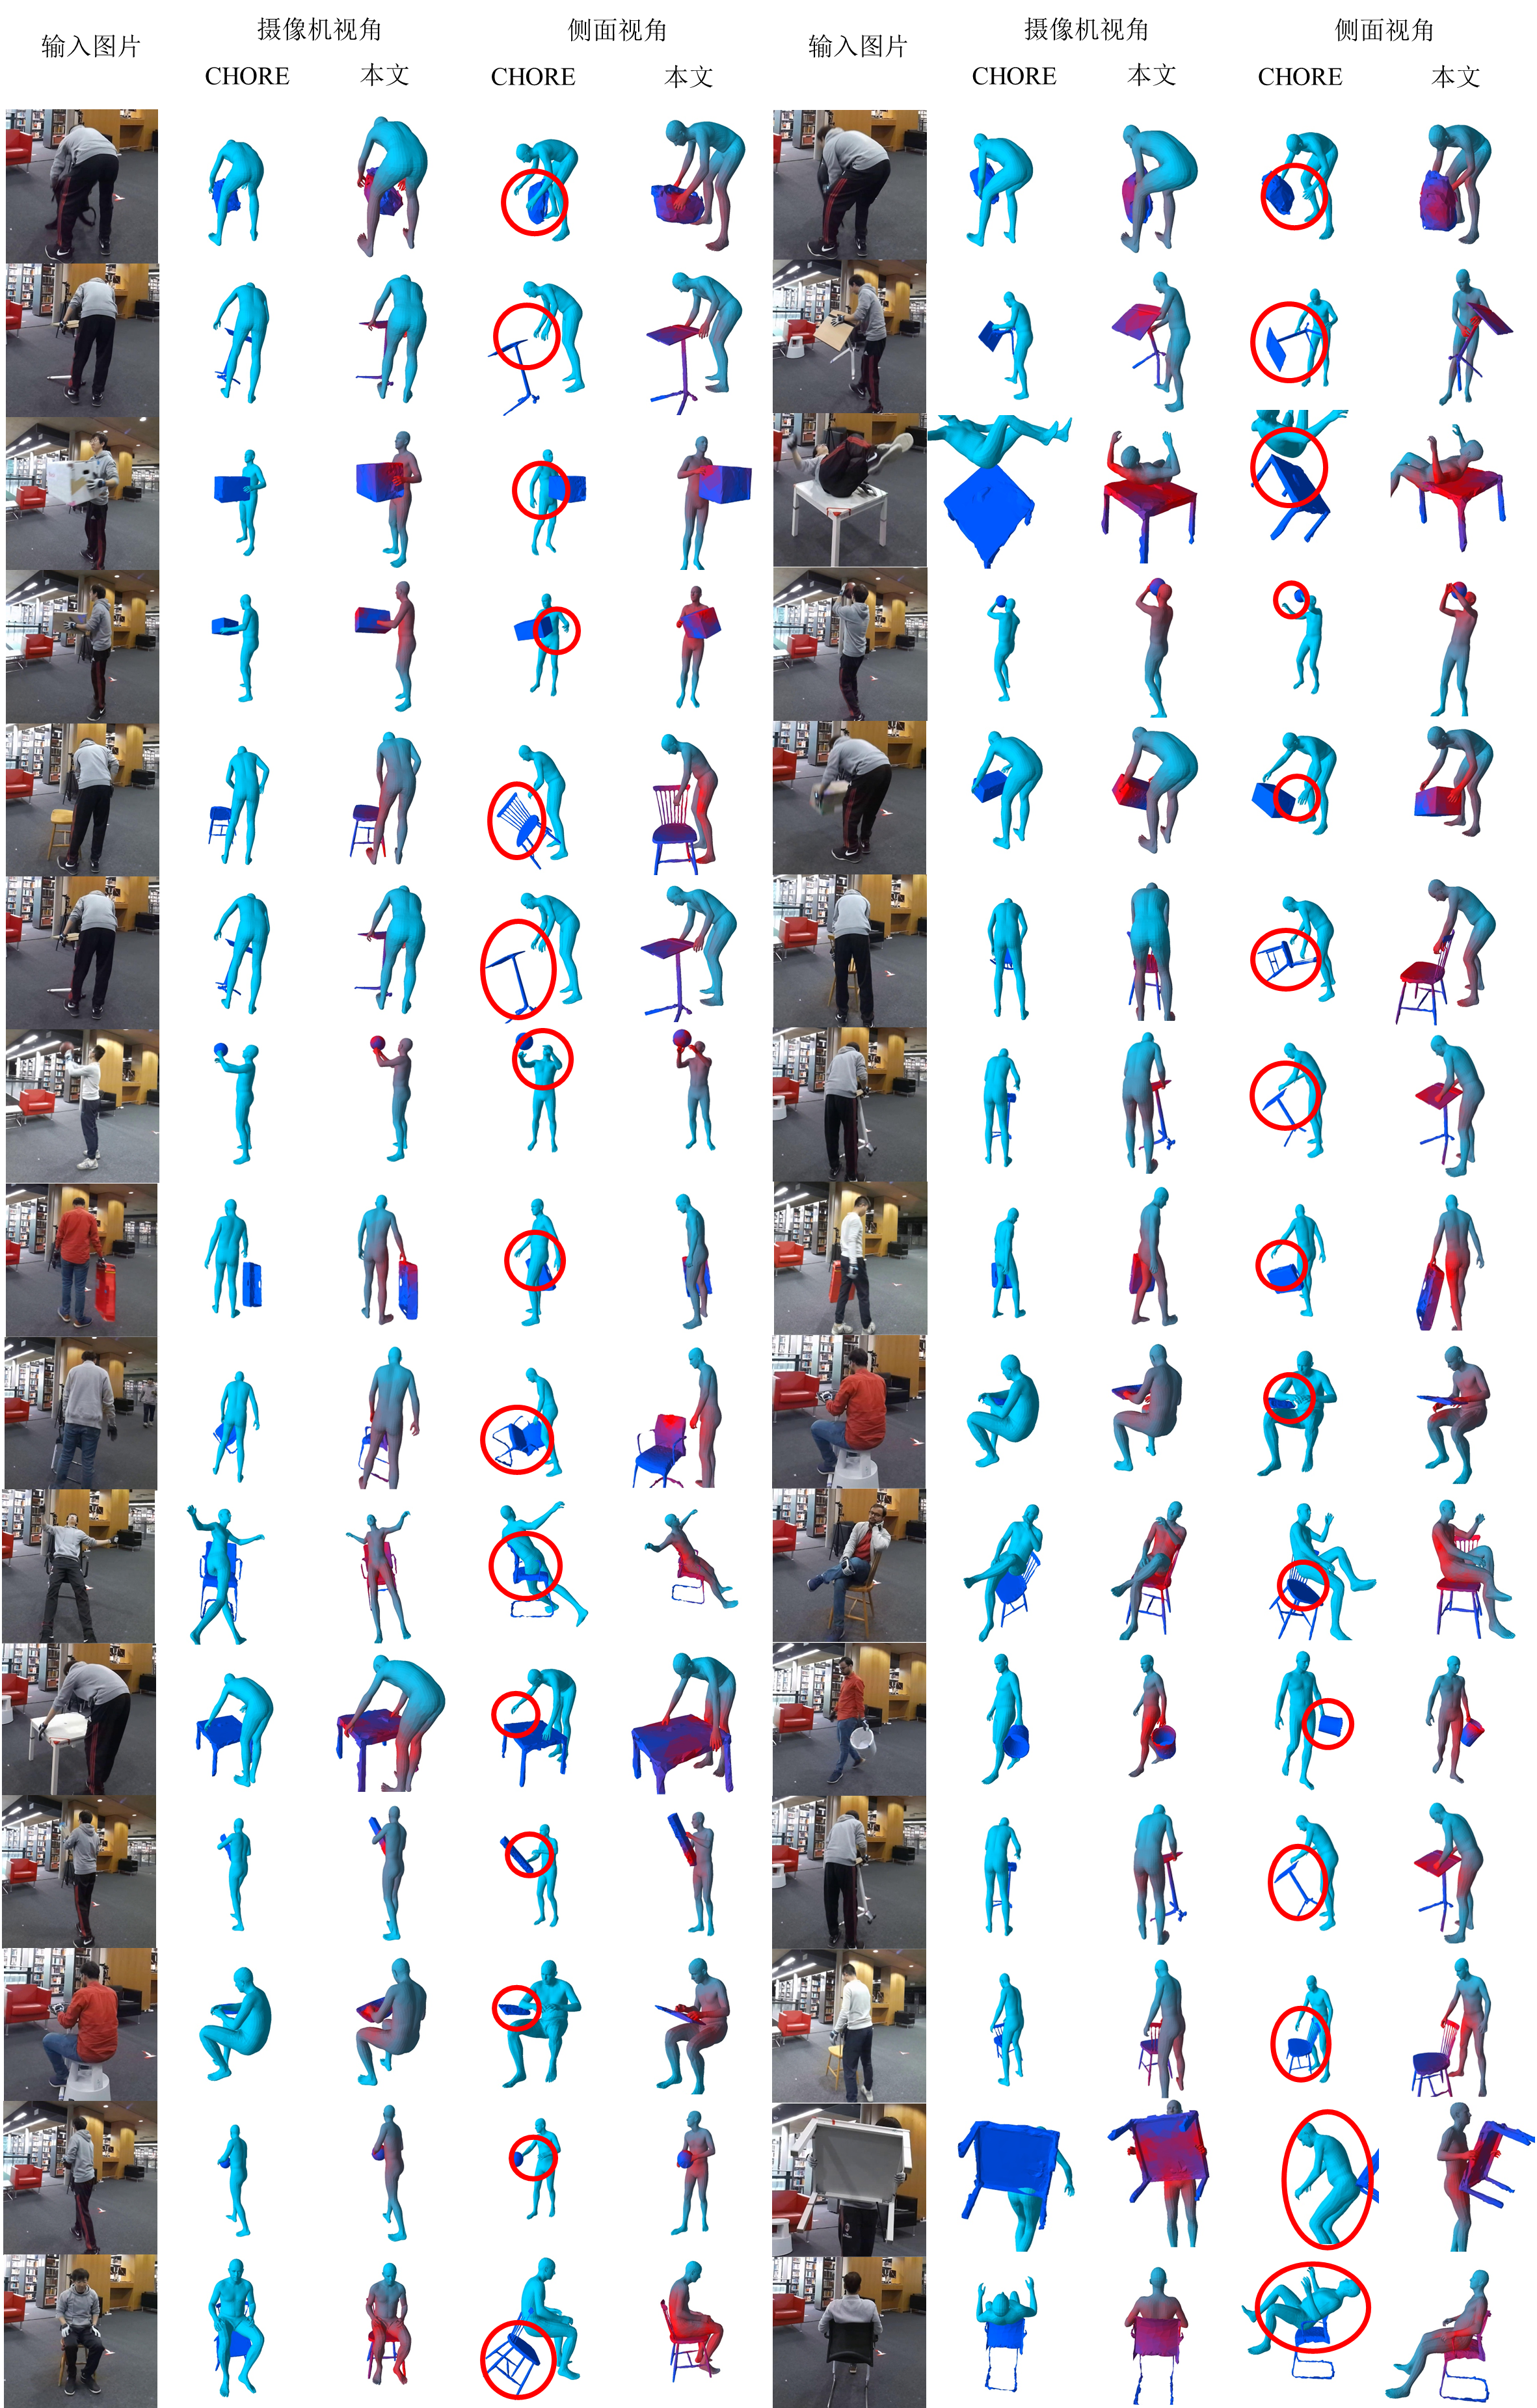
\includegraphics{Img/comparison_stackflow}
	\bicaption{本章所提出的方法和CHORE在BEHAVE数据集上的定性对比。}{Quantization comparison between our method and CHORE on BEHAVE dataset.}
	\label{fig:comparison-with-chore}
\end{figure}

\subsection{消融实验}
为验证提出的所基于偏移量表征的对人-物空间关系编码的信息保真度,设计以下实验。对每一个人-物交互实例按照章节\ref{sec:offset-representation}提取人-物空间关系编码$\mathbf{\gamma}$,使用反投影(式(\ref{eq:reproject-offset}))得到偏移量$\mathbf{d}$,之后从$\mathbf{d}$中按照式(\ref{eq:recon_from_offset})重构出参数$\{\mathbf{\beta}, \mathbf{\theta}, \mathbf{R}, \mathbf{t}\}$,人体模型表面顶点$\mathbf{P}^{\text{h}}$从$\mathbf{\beta}, \mathbf{\theta}$中重构出,而物体表面顶点$\mathbf{P}^{\text{o}}$从$\mathbf{R}, \mathbf{t}$重构出,计算重构出的参数和标签之间的$\ell$-1距离,得到表\ref{tab:ablation_anchor_num}中的结果。从表中可以看出,基于偏移量对信息保存完整,重构出的人的顶点误差和物的顶点平均误差均在1cm内,$\mathbf{\gamma}$的维度对重建误差具有较大的影响,高纬度的$\mathbf{\gamma}$对信息保存更完整,但高纬度$\mathbf{\gamma}$会带来额外的计算开销。人体锚点数量$m$和物体锚点数量$n$对重建结果影响并不明显,这是由于物体网格模型和人体网格模型中顶点存在一定的相互约束,即使使用少量的锚点也能得到和使用大量锚点相媲及的重建精度。

\begin{table}[!htbp]
	\bicaption{\centering{人-物网格模型表面锚点数量和隐式空间的维度对重建误差的影响。}}{\centering{The influence of the number of the human anchors, object anchors and the dimension of the latent relation space to the reconstruction accuracy.}}
	\label{tab:ablation_anchor_num}
	\centering
	\footnotesize
	\setlength{\tabcolsep}{4pt}
	\renewcommand{\arraystretch}{1.2}
	\begin{tabular}{c|c|cccc|cccc|cccc}
		\toprule
		\multirow{3}{*}{超参数} & $k$ & \multicolumn{4}{c}{32} & \multicolumn{4}{c}{64} & \multicolumn{4}{c}{128} \\
		\cline{2-14}
		& $m$ & 88 & 176 & 352 & 704 & 88 & 176 & 352 & 704 & 88 & 176 & 352 & 704 \\
		& $n$ & 8 & 16 & 32 & 64 & 8 & 16 & 32 & 64 & 8 & 16 & 32 & 64 \\
		\hline
		\multirow{7}{*}{重建误差} & $\mathbf{\beta}$ & 0.554 & 0.567 & 0.596 & 0.596 & 0.359 & 0.321 & 0.316 & 0.319 & 0.297 & 0.243 & 0.230 & 0.235 \\
		& $\mathbf{\theta}$ & 0.138 & 0.121 & 0.117 & 0.119 & 0.090 & 0.070 & 0.063 & 0.067 & 0.064 & 0.042 & 0.037 & 0.044 \\
		& $\mathbf{R}$ & 0.044 & 0.039 & 0.018 & 0.018 & 0.060 & 0.025 & 0.022 & 0.018 & 0.050 & 0.044 & 0.033 & 0.020 \\
		& $\mathbf{t}$ & 0.006 & 0.006 & 0.005 & 0.006 & 0.003 & 0.002 & 0.002 & 0.002 & 0.003 & 0.002 & 0.001 & 0.001 \\
		& $\mathbf{P}^{\text{h}}$ & 0.009 & 0.009 & 0.009 & 0.009 & 0.003 & 0.003 & 0.002 & 0.002 & 0.002 & 0.001 & 0.001 & 0.002 \\
		& $\mathbf{P}^{\text{o}}$ & 0.008 & 0.008 & 0.006 & 0.006 & 0.005 & 0.003 & 0.003 & 0.002 & 0.005 & 0.004 & 0.003 & 0.002 \\
		& $\mathbf{d}$ & 0.008 & 0.007 & 0.007 & 0.007 & 0.002 & 0.002 & 0.002 & 0.002 & 0.000 & 0.000 & 0.001 & 0.001 \\
		\bottomrule
	\end{tabular}
\end{table}

进一步,在表\ref{tab:ablation_representation}中,对比了隐向量$\mathbf{\gamma}$维度、人体锚点数量$m$和物体锚点数量$n$在实际应用到重建任务中后对重建精度的影响。从表中可以看出,选取的锚点数量越多重建精度越高,但提升微乎其微。在$\mathbf{\gamma}$使用较大的维度后,结果提升不如期望,这是由于较高的维度会带来模型参数的变多,进而影响训练过程,从而在测试集的表现不如预期。

\begin{table}[!htbp]
	\bicaption{\centering{隐向量$\mathbf{\gamma}$维度、人体锚点数量$m$和物体锚点数量$n$对重建结果的影响。}}{\centering{The effectiveness of the number of the dimension of $\mathbf{\gamma}$, $m$ and $n$ to the reconstruction accuracy.}}
	\label{tab:ablation_representation}
	\centering
	\footnotesize
	\setlength{\tabcolsep}{4pt}
	\renewcommand{\arraystretch}{1.2}
	\begin{tabular}{c|c|ccc|c|c}
		\toprule
		\multirow{3}{*}{超参数} & $k$ & \multicolumn{3}{c|}{32} & 64 & 128 \\
		\cline{2-7}
		& $m$ & 176 & 352 & 704 & 704 & 704 \\
		& $n$ & 16 & 32 & 64 & 64 & 64 \\
		\hline
		\multirow{2}{*}{重建误差} & 人体 & 4.95 & 4.88 & 4.79 & \textbf{4.71} & 4.73 \\
		& 物体 & 9.47 & 9.32 & \textbf{9.12} & 9.87 & 10.88 \\
		\bottomrule
		\multicolumn{6}{l}{注:加粗字体为最优结果。}
	\end{tabular}
\end{table}

在表\ref{tab:ablation_loss}中,对比了联合优化中各个损失对重建结果的影响,其中$\mathcal{L}_{\text{SMPL}}$是对于人体的损失,具体包含人体关键点的重投影损失,即式(\ref{eq:joint_loss})中的$\mathcal{L}_{\mathbf{J}}$,还包括式(\ref{eq:nll-optim})中的对人体姿态的负对数似然$-\ln p_{\Theta|I}(\mathbf{\theta}|\mathbf{c})$的损失。损失$\mathcal{L}_{\text{object}}$是物体的坐标重投影损失,即式(\ref{eq:coor_reprojection})中的$\mathcal{L}_{\text{coor}}$。$\mathcal{L}_{\text{offset}}$是对人和物体之间偏移量的损失即式(\ref{eq:nll-optim})中人-物关系的负对数似然$ - \ln p_{\Gamma|I,\Theta}(\mathbf{\gamma}|\mathbf{c}, \mathbf{\theta})$。人体和物体的重建误差使用和标签的倒角距离衡量,从表中结果可以看出,这三类损失均对重建精度有重要影响,缺一不可,只有共同作用才联合优化上,才能达到最优秀的重建精度。

\begin{table}[!htbp]
	\bicaption{联合优化过程中各个损失对重建结果的影响。}{The effectiveness of different optimization losses on the reconstruction accuracy.}
	\label{tab:ablation_loss}
	\centering
	\footnotesize
	\setlength{\tabcolsep}{4pt}
	\renewcommand{\arraystretch}{1.2}
	\begin{tabular}{ccc|cc}
		\toprule
		\multirow{2}{*}{$\mathcal{L}_{\text{SMPL}}$} & \multirow{2}{*}{$\mathcal{L}_{\text{object}}$} & \multirow{2}{*}{$\mathcal{L}_{\text{offset}}$} & \multicolumn{2}{c}{重建误差} \\
		\cline{4-5}
		&&& 人体 & 物体 \\
		\hline
		\XSolidBrush & \Checkmark & \Checkmark & 8.81 & 16.42 \\
		\Checkmark & \XSolidBrush & \Checkmark & 5.22 & 13.84 \\
		\Checkmark & \Checkmark & \XSolidBrush & 5.24 & 16.95 \\
		\Checkmark & \Checkmark & \Checkmark & \textbf{4.79} & \textbf{9.12} \\
		\bottomrule
		\multicolumn{5}{l}{注:加粗字体为最优结果。}
	\end{tabular}
\end{table}

在表\ref{tab:ablation_augment}中,对比了在使用不同比例的增强数据集对重建结果的影响,表中$\alpha$是增强数据集中用于训练的比例,使用全部的增强数据集训练的模型达到了最高的重建精度(表\ref{tab:ablation_augment}中最后一行),注意到使用全部增强数据和使用一半增强数据的重建指标限差微乎其微,这说明合适的增强数据的比例在0.5-1之间,在生成增强数据集的过程中,摄像机环绕人体一圈,每隔角度$360^\circ / 12 = 30^\circ$渲染一张图片,而增强数据集的比例$0.5$对应于间隔角度为$60^\circ$,这说明在生成数据集时合适的角度为$60^\circ$。

\begin{table}[!htbp]
	\bicaption{\centering{使用不同比例的增强数据对重建结果的影响。}}{\centering{The impact of different fractions of augmentated dataset on the reconstruction accuracy.}}
	\label{tab:ablation_augment}
	\centering
	\footnotesize
	\setlength{\tabcolsep}{4pt}
	\renewcommand{\arraystretch}{1.2}
	\begin{tabular}{c|cccccc}
		\toprule
		$\alpha$ & 0.00 & 0.17 & 0.25 & 0.33 & 0.50 & 1.00 \\
		\hline
		人体 & 4.60 & 4.39 & 4.40 & 4.37 & \textbf{4.33} & \textbf{4.33} \\
		物体 & 9.83 & 9.11 & 9.14 & 9.03 & 8.88 & \textbf{8.87} \\
		\bottomrule
		\multicolumn{6}{l}{注:加粗字体为最优结果。}
	\end{tabular}
\end{table}

\subsection{单人多物交互拓展}
虽然在实验中,本章所提出的使用偏移量来调节人体和物体之间的空间关系的方法是应用于单人单物场景,但本章所提出的算法可以拓展对单人多物的场景中,在单人多物场景中,人的位姿受与之交互的各种物体约束,将多个物体对人体的偏移量同时作用在人体上来共同优化。在图\ref{fig:stackflow_multi_object}中展示了本章算法应用到单人多物场景中的重建结果。

\begin{figure}[htbp]
	\centering
	\includegraphics{Img/stackflow_multi_object}
	\bicaption{\centering{StackFLOW应用在单人多物场景中的重建结果。}}{\centering{The qualitative results of the StackFLOW applied to the interaction between single-person and multi-object.}}
	\label{fig:stackflow_multi_object}
\end{figure}

\section{本章小结}
本章提出了一种基于人-物偏移量对人和物体之间空间关系的刻画方式,并将该刻画方式应用在人-物重建问题上。通过计算人和物体之间偏移量,更加准确地描述人和物体之间的相对位置关系,这种刻画方式的优势在于可以将人体和物体用同一个量描述,从而更加方便进行对人-物之间的空间关系的分析和建模。为了将该基于偏移量刻画方式应用到人-物重建问题上,本章还给出了一种预测-优化的两阶段重建算法。在预测阶段,使用叠层归一化流模型预测给定图片的人-物空间关系的后验分布,在后优化阶段,结合重投影损失和该后验分布的损失微调结果。在BEHAVE数据集上的实验结果证明了该方法的有效性,该方法和基于隐式向量场或者基于接触面的方法相比具有更高的重建精度和运行效率,并且对于严重遮挡的情况具有更高的鲁棒性。

尽管本章所提出的方法在BEHAVE数据集取得了很不错的结果,但仍然存在一些局限性。首先,本章所提出的方法是建立在物体网格模型已知的前提下,该方法只能应用于包含指定物体的人-物重建,在这种限制导致该方法不能应用到大多数场景中。其次,该方法在构建人和物体空间关系的隐式表达时,需要预先在人体和物体网格模型选择锚点并且进行PCA降维处理,这种以离线形式所构建的隐式人-物交互关系空间不能在后续动态调整,不是端到端的方式。最后,本章所提出的算法泛化能力较差,该方法由于将图片作为一种条件输入到叠层归一化流中,因此对于训练集差距较大的自然场景中的图片,该方法泛化能力较差。

针对这些局限性,未来的工作可以探索以下几个方向进行改进和优化:
\begin{itemize}
	\item 扩展到无网格模型的场景:可以考虑将方法扩展到无网格模型的情况下,通过学习更加通用的人体和物体表示来解决这个问题。这样可以使方法更具有普适性,适用于更广泛的场景。
	\item 端到端学习:将人体和物体之间的空间关系的表达方式改为端到端学习,可以更好地动态调整人-物交互空间表示,提高方法的灵活性和准确性。
	\item 提高泛化性能:可以通过引入更多的数据增强技术,或者修改网络结构,使其更好地适应不同风格和场景的图片,从而提高方法的泛化能力。
\end{itemize}
通过以上不断的改进和优化,可以使基于人-物偏移量的空间关系刻画方法在人-物重建问题上取得更好的效果,并且在实际应用中发挥更大的作用。
\chapter{人和物体交互的域内泛化}\label{chap:stackflow_plus}
开放场景中的物体形状具有较高多样性,学习如何跟未曾见过物体交互对算法能否应用到自然场景中至关重要,前置章节所提出的算法从数据集中学习实例级别的交互先验,并在测试时只能将从训练集学习到的先验应用到相同的物体中,对于未曾见过的物体泛化能力较差。为了克服该泛化能力弱的缺陷,本章提出基于种类级别的交互先验学习算法,该算法构建出物体形状归一化映射,将物体映射到统一的形状空间中,在该形状空间中建立人和物体之间的交互关系。在CHAIRS数据集上的实验表明,该算法对同类别的未曾见过的物体仍然保持很强的泛化能力。

\section{人-物交互关系的先验空间构建}

给定物体$O = (\hat{\mathbf{V}}^{\text{o}}, \mathbf{E}^{\text{o}})$,章节\ref{sec:offset-representation}提出基于偏移量的编码方式来刻画人与该物体交互时的三维空间关系,对每一个以$\{\mathbf{\beta}, \mathbf{\theta}, \mathbf{R}, \mathbf{t}\}$为参数人-物交互实例,计算锚点之间的偏移量,并利用特征值分解的方式将偏移量映射到隐式空间中,得到基于偏移量的表征$\mathbf{\gamma}$,即
\begin{equation}
	\mathbf{\gamma} = R_{O} (\mathbf{\beta}, \mathbf{\theta}, \mathbf{R}, \mathbf{t}),
\end{equation}
式中,$R_{O}$是物体$O$的空间关系编码函数,该种基于人-物锚点偏移量的编码方式建立在物体$O$的拓扑结构已知的前提下,对于未曾见过的其它形状的物体失效。为了解决对其它物体泛化能力差的问题,本节提出使用物体形状映射函数$D$将物体归一化到和交互相关联的形状空间$\mathcal{O}$中,在该空间中,物体的形状被归一化,其拓扑结构只被保留和人交互中最相关的部位。而后将人和物体空间关系的编码函数$R_{\mathcal{O}}$建立在该形状空间之上,即使对于未曾见过的物体$O'$,在经过形状映射函数$D$之后得到了对物体形状的统一化表达,而人和物体间交互编码建立在$\mathcal{O}$之上,因而对于未见过的$O'$也保持强泛化能力。

\subsection{物体归一化映射函数}
人总是和物体特定的位置交互,同类物体的形状虽千奇百怪,但其内在却存在相似的拓扑结构和统一的可交互部位,为提取物体中和交互相关联的部位,使用物体形状归一化映射函数$D$,该函数将物体形状映射到与交互相关联的形状空间$\mathcal{O}$中。

如图\ref{fig:learn-object-inter-shape}所示,给定物体$O=(\hat{\mathbf{V}}^\text{o}, \mathbf{E}^{\text{o}})$,使用体素编码器$E$提取物体的形状特征$\mathbf{c}$,
\begin{equation}
	\mathbf{c} = E(\mathbf{O}),
\end{equation}
式中,$\mathbf{O}\in \mathbb{R}^{N\times N \times N}$是从物体$O$中提取的体素网格(voxel grid),$N\in \mathbb{N}$为该体素的分辨率,体素编码器$E$是由多层3D卷积网络构成,最后使用池化层对体素特征降采样得到物体的形状编码$\mathbf{c}$。形状映射函数$D$是由一组级联的网格模型形变器组成,该网格模型形变器从初始椭球体$\mathcal{S}=(\hat{\mathbf{S}}^{(0)}, \mathbf{E}^{\mathcal{S}})$出发,逐步对椭球体初始顶点$\hat{\mathbf{S}}^{(0)}$添加偏置,最终得到物体目标形状$D(\mathbf{O})=(\hat{\mathbf{S}}^{\star}, \mathbf{E}^{\mathcal{S}})$。每一层网格模型形变器由基于残差连接的图卷积层构成,以上一层的顶点作为输入,产生下一层的顶点,即
\begin{equation}
	\hat{\mathbf{S}}^{(i+1)} = \text{G-ResNet}(\hat{\mathbf{S}}^{(i)} \oplus \mathbf{c}, \mathbf{E}^{\mathcal{S}}),
\end{equation}
式中,G-ResNet为基于残差连接的图卷积网络\citep{Pixel2Mesh},$\oplus$表示特征按照维度相连接,$\mathbf{c}$是从物体$O$提取的特征,$\mathbf{E}^{\mathcal{S}}$为初始椭球体的边。归一化后的物体网格模型$D(\mathbf{O})=(\hat{\mathbf{S}}^\star, \mathbf{E}^{\mathcal{S}})$共享一组边集,并且具有相同数量的顶点。

\begin{figure}[!htbp]
	\centering
	\includegraphics{Img/learn_object_shape}
	\bicaption{学习物体形状归一化映射流程图。}{The pipeline of the procedure of learning interaction-relatied shape mapping.}
	\label{fig:learn-object-inter-shape}
\end{figure}

\subsection{人物关系编码}
在章节\ref{sec:offset-representation}提出的编码方式中,物体锚点采样于特定形状物体的网格模型表面,使用该锚点对应的偏移量所构建的隐式空间只能作用于该物体,不能泛化到其他形状的物体,而本章所提出的编码方式中,物体的锚点采样于初始椭球体$\mathcal{S}$,所有物体经过归一化映射之后,网格模型顶点数量相同且具有相同的拓扑连接结构,因而锚点索引集合可以被所有物体共享。从物体的初始椭球体$\mathcal{S}$表面均匀随机选取$n$个点,记录该$n$个点的索引形成物体的锚点索引集合$\mathcal{A}_{\mathcal{O}}$,对于每一个物体$O$,其锚点取自于形状归一化后的物体模型$D(\mathbf{O})$,人体锚点的选取方式和章节\ref{sec:offset-representation}保持一致。偏移量计算方式由式(\ref{eq:offset})改成
\begin{equation}
	\mathbf{d}_{i,j} = \mathbf{S}^{\star}_j - \mathbf{V}_i^{\text{h}}, i \in \mathcal{A}_{\text{h}}, j \in \mathcal{A}_{\mathcal{O}},
\end{equation}
式中,$\mathbf{S}^\star_j = \mathbf{R} \hat{\mathbf{S}}^\star_j + \mathbf{t}$为物体归一化后的顶点在SMPL模型局部坐标系下的坐标。在该种计算方式下,人-物交互实例对应的空间关系编码会随着物体映射函数$D$的变化而变化,使用增量式主成分分析\citep{Ross2008IncrementalLF}来自适应学习人物空间关系编码,该增量式学习的过程伴随物体映射函数$D$学习的过程,增量式主成分分析逐步从数据中学习空间投影矩阵$\mathbf{P}$和数据均值$\mathbf{\mu}$。在增量式学习空间关系编码过程中,对于每一批次的偏移量$\mathbf{X}_{\text{batch}} \in \mathbb{R}^{p \times 3mn}$,计算矩阵$[f\mathbf{\Sigma} \mathbf{P}^T,\\ \mathbf{X}_{\text{batch}} - \bar{\mathbf{X}}_{\text{batch}}, \sqrt{\frac{pq}{p + q}}(\bar{\mathbf{X}}_{\text{batch}} - \mathbf{\mu})]$的奇异值分解,即
\begin{equation}
	\hat{\mathbf{U}}\hat{\mathbf{\Sigma}}\hat{\mathbf{V}}^T = \text{SVD}([f\Sigma \mathbf{P}^T, \mathbf{X}_{\text{batch}} - \bar{\mathbf{X}}_{\text{batch}}, \sqrt{\frac{pq}{p + q}}(\bar{\mathbf{X}}_{\text{batch}} - \mathbf{\mu})]),
\end{equation}
式中,$\bar{\mathbf{X}}_{\text{batch}}$表示当前批次偏移量的均值,$p$为当前批次样本个数,$q$表示截至目前所迭代过样本的总数,$f$是遗忘因子,$\mathbf{\Sigma}$为投影矩阵$\hat{\mathbf{P}}$中各个维度的方差,经奇异值分解后,取$\hat{\mathbf{\Sigma}}$前$k$个较大的方差和$\mathbf{V}$中对应的向量来更新$\mathbf{\Sigma}$和$\mathbf{\mathbf{P}}$,均值向量$\mathbf{\mu}$按照下式更新,
\begin{equation}
	\mathbf{\mu} \gets \frac{p}{p + fq} \bar{\mathbf{X}}_{\text{batch}} + \frac{fq}{p + fq}\mathbf{\mu}.
\end{equation}

投影矩阵$\mathbf{P}$和数据的均值$\mathbf{\mu}$伴随着物体映射函数的学习,在物体映射函数的学习过程中,人和物体之间的偏移量会随着被映射后的物体的形状而逐步变化,$\mathbf{P}$和$\mathbf{\mu}$会伴随物体的形状而逐步更新。

\subsection{训练}
训练该形状映射函数$D$的损失函数包含网格模型平滑损失、人物交互损失和特征分解损失。为了提取物体和人体交互最相关的区域,对人和物体频繁交互的区域做出损失,使得物体在映射后形状能够保持其可交互的特性。记$d(\mathbf{v}, \mathbf{V})$为点$\mathbf{v}$到点集$\mathbf{V}$的最短距离,与人相交互的损失为
\begin{equation}
	\mathcal{L}_{\text{inter}} = \sum_{\mathbf{v} \in \mathbf{V}^{\text{h}}} w(\mathbf{v}) \cdot \| d(\mathbf{v}, \mathbf{V}^{\text{o}}) - d(\mathbf{v}, \mathbf{S}^{\star}) \|_1,
\end{equation}
式中,$w(\mathbf{v})$的在点$\mathbf{v}$处的权重,其计算方式为
\begin{equation}\label{eq:weighting}
	w(\mathbf{v}) = f(d(\mathbf{v}, \mathbf{V}^\text{o})) + f(d(\mathbf{v}, \mathbf{S}^\star)) - f(d(\mathbf{v}, \mathbf{V}^\text{o})) \cdot f(d(\mathbf{v}, \mathbf{S}^\star)),
\end{equation}
式中$f(x) = (\alpha x + 1) \cdot e^{- \alpha x}$为权重函数,$\alpha$为大于0的常数,当$x\to 0^+$,$f(x) \to 1$,当$x\to +\infty$,$f(x)\to0$。式(\ref{eq:weighting})计算权重的方式很好的平衡了那些和交互关联度高的点和外围点,当点$\mathbf{v}$处于交互区域,即该点距离物体网格模型较近,$f(\mathbf{v}, \mathbf{V}^{\text{o}}) \simeq 1$,$w(\mathbf{v}) \simeq 1$,此时损失促使$\mathbf{S}^\star$和目标物体$\mathbf{V}^\text{o}$的对应部分相匹配,相反如果点$\mathbf{v}$处于非交互区域,此时点$\mathbf{v}$周围应该处于空区域,$f(d(\mathbf{v}, \mathbf{V}^\text{o})) \simeq 0, w(\mathbf{v}) \simeq f(d(\mathbf{v}, \mathbf{S}^\star))$,损失会促使$\mathbf{S}^\star$远离该点以防发生穿模。

为了使重建后的模型能够保持平滑,使用平滑损失
\begin{equation}
	\mathcal{L}_\text{smooth} = \mathcal{L}_{\text{edge}} + \mathcal{L}_{\text{mesh}},
\end{equation}
式中,$\mathcal{L}_{\text{edge}} = \sum_{(u, v) \in \mathbf{E}^{\mathcal{S}}} \| \mathbf{S}^\star_u - \mathbf{S}_v^\star \|$,$\mathcal{L}_{\text{mesh}}$为网格模型的拉普拉斯平滑损失,其具体形式参照\citep{Nealen2006LaplacianMO}。

章节\ref{sec:offset-representation}为了构建隐式空间使用离线主成分分析,该离线主成分分析是构建在物体形状已知的前提下。而在本章中,物体形状是由映射函数$D$得到的,为此使用增量式主成分分析\citep{Ross2008IncrementalLF}学习投影矩阵$\mathbf{P}$和均值向量$\mathbf{\mu}$。在增量式主成分分析中,$\mathbf{P}$和$\mathbf{\mu}$随物体映射函数的改变而改变,为了使物体映射函数能够重构出和交互相关的形状,并且约束隐式空间,最小化投影函数$\mathbf{P}$的核范数,即
\begin{equation}
	\mathcal{L}_{\text{PCA}} = \| \mathbf{P} \|_*.
\end{equation}
因此,在训练物体形状映射函数和构建隐式空间阶段时的损失为
\begin{equation}
	\mathcal{L} = \lambda_{\text{inter}} \mathcal{L}_{\text{inter}} + \lambda_{\text{smooth}} \mathcal{L}_{\text{smooth}} + \lambda_{\text{PCA}} \mathcal{L}_{\text{PCA}}.
\end{equation}
在实验中,$\lambda_{\text{inter}} = \lambda_{\text{smooth}} = 1, \lambda_{\text{PCA}} = 1e-4$。

\section{重建算法}
将学习得到的物体形状归一化映射函数和基于偏移量的人-物空间编码应用到人-物重建任务中,为建立图片和人-物空间关系的映射,采用章节\ref{sec:stackflow}提出的叠层归一化流结构。使用预先训练好的物体形状归一化映射函数将物体的形状映射到形状空间$\mathcal{O}$,并使用主成分分析提取人-物空间关系的特征$\mathbf{\gamma}$,使用提取的特征训练归一化流模型,使其从数据集中学习概率密度$p_{\Gamma|\mathcal{I}}(\mathbf{\gamma}|\mathbf{c})$,训练归一化流模型时,物体形状归一化映射函数和人-物空间编码保持不变。在预测过程中,使用该归一化流模型从给定的图片中建立人-物空间关系的概率密度,并按照式(\ref{eq:gamma-prediction})取概率密度最大的空间关系作为最终预测结果。

\section{实验结果与分析}

\subsection{数据集以及评测指标}
本章采用CHAIRS数据集\citep{Jiang2022FullBodyAH}测试算法对未曾见过物体的泛化能力。CHAIRS数据集是在实验室环境中采集的人和椅子交互的数据集,数据集给出了多视角的RGB-D视频序列以及每一帧的人和物体网格模型的三维标注,包含46位参与者和81把椅子之间的交互。官方发布了包含人和60把不同形状椅子的交互,实验中选取其中9把椅子用于测试,其它51把椅子用于训练。为了更加公平比较人-物空间关系重建的精度和对未知物体的泛化能力,测试时使用了人体SMPL的标签,只比较物体位姿的重建精度。在实验中,采用了和\citep{Jiang2022FullBodyAH}相同的测评指标,为了衡量物体位姿的精度,采用物体的旋转重建误差、位置重建误差和物体的倒角距离。为了评测人和物体之间空间关系,采用穿模损失和接触损失,穿模损失是指物体插入人体网格模型的最大深度,而接触损失是指物体网格模型和人体网格模型的最短距离,该距离被裁剪到0到20cm,对每张测试图片计算上述指标,取平均作为最终指标。

\subsection{定量分析}
为验证本章所提出的方法能够学习到物体和人体交互相关的形状映射函数,并且能够对未曾见过的物体产生泛化能力,将本文提出的基于偏移量的方法(记为offset-based)和基于物体6D位姿估计的方法(记为RT-based)进行了对比。基于6D位姿的方法直接预测物体相对于人体的旋转和平移,相反基于偏移量的方法预测人-物空间编码$\mathbf{\gamma}$,两者在CHAIRS数据集上的指标如表\ref{tab:comparison_chairs}所示,能够很清楚看出,基于偏移量对未曾见过的物体泛化能力更强,由于基于偏移量的方法预测的是和人体交互相关的偏移量,该偏移量是由归一化后的物体形状和人体计算得到的,和特定的物体形状无关,因而能够更好地迁移到其它形状的物体上,而基于6D位姿的方法直接预测的6D位姿是依赖于物体的形状的,即同一个交互由于物体的形状不同而导致物体的6D位姿有差异,因而对未曾见过的物体泛化能力不如基于偏移量的方法。

\begin{table}[!htbp]
	\bicaption{\centering{基于偏移量的方法和基于6D位姿的方法在CHAIRS数据集上的指标对比。}}{\centering{The comparison between the offset-based method and the RT-based method on CHAIRS dataset.}}
	\label{tab:comparison_chairs}
	\centering
	\footnotesize
	\setlength{\tabcolsep}{4pt}
	\renewcommand{\arraystretch}{1.2}
	\begin{tabular}{lccccc}
		\toprule
		\multirow{2}{*}{方法} & \multicolumn{3}{c}{Object} & \multicolumn{2}{c}{HOI} \\
		& Rot.($^\circ$) & Transl.(cm) & CD(cm) & Pene.(cm) & Cont.(mm) \\
		\hline
		RT-based & 27.27 & 12.77 & 12.69 & 2.83 & 23.55 \\
		Offset-based & \textbf{20.83} & \textbf{11.94} & \textbf{9.72} & \textbf{2.41} & \textbf{15.81} \\
		\bottomrule
		\multicolumn{6}{l}{注:加粗字体为最优结果。}
	\end{tabular}
\end{table}

为探究在训练物体形状映射函数时,不同损失对重建结果的影响,做如下实验,在训练物体映射函数逐个剔除其中某个损失,将训练得到的物体映射函数应用在人-物重建上并在测试集对比重建精度,得到表\ref{tab:training_loss_chairs}所示的结果,结果表明,损失$\mathcal{L}_{\text{PCA}}$对结果的影响最大,通过最小化增量PCA中的投影矩阵的核范数的损失$\mathcal{L}_{\text{PCA}}$能够使使增量PCA学习过程能够提取到最稀疏的特征表达,从而使得模型产生更强的泛化能力。

\begin{table}[!htbp]
	\bicaption{\centering{训练物体形状映射函数的不同损失对重建结果的影响。}}{\centering{The effectiveness of different losses during training the object shape mapping on the reconstruction accuracy.}}
	\label{tab:training_loss_chairs}
	\centering
	\footnotesize
	\setlength{\tabcolsep}{4pt}
	\renewcommand{\arraystretch}{1.2}
	\begin{tabular}{cccccccc}
		\toprule
		\multirow{2}{*}{$\mathcal{L}_{\text{inter}}$} & \multirow{2}{*}{$\mathcal{L}_{\text{smooth}}$} & \multirow{2}{*}{$\mathcal{L}_{\text{PCA}}$} & \multicolumn{3}{c}{Object} & \multicolumn{2}{c}{HOI} \\
		& &  & Rot.($^\circ$) & Transl.(cm) & CD(cm) & Pene.(cm) & Cont.(mm) \\
		\hline
		\XSolidBrush & \Checkmark & \Checkmark & 22.86 & 11.82 & 10.52 & 2.50 & 17.73 \\
		\Checkmark & \XSolidBrush & \Checkmark & \textbf{16.77} & \textbf{10.74} & \textbf{9.56} & 2.77 & 17.47 \\
		\Checkmark & \Checkmark & \XSolidBrush & 30.43 & 14.73 & 13.01 & 2.96 & 16.33 \\
		\Checkmark & \Checkmark & \Checkmark & 26.40 & 11.30 & 10.51 & \textbf{2.29} & \textbf{15.75} \\
		\bottomrule
		\multicolumn{6}{l}{注:加粗字体为最优结果。}
	\end{tabular}
\end{table}

在表\ref{tab:alpha_on_chairs}中和图\ref{fig:alpha_shape},对比了损失$\mathcal{L}_{\text{inter}}$中的参数$\alpha$对重建精度的影响,当$\alpha$取值较小时,式(\ref{eq:weighting})中只有当物体模型表面上的点和人体模型表面上的点之间距离$d(\mathbf{v}, \mathbf{V}^{\text{o}})$很近时,才会拉近$\mathbf{v}$和$\mathbf{S}^\star$的距离,同时大多数情况$w(\mathbf{v})$接近于0,因此损失$\mathcal{L}_{\text{inter}}$会使模型学习到更细粒度的形状。相反如果$\alpha$取值较大,$w(\mathbf{v})$更偏向于1,会使得模型学习物体更粗粒度的形状。从表\ref{tab:alpha_on_chairs}中可以看出,越大的$\alpha$的取值会带来更小的物体重建误差。

\begin{table}[!htbp]
	\bicaption{损失$\mathcal{L}_{\text{inter}}$中的参数$\alpha$对重建结果的影响。}{The effectiveness of $\alpha$ on the reconstruction accuracy.}
	\label{tab:alpha_on_chairs}
	\centering
	\footnotesize
	\setlength{\tabcolsep}{4pt}
	\renewcommand{\arraystretch}{1.2}
	\begin{tabular}{cccccc}
		\toprule
		\multirow{2}{*}{$\alpha$} & \multicolumn{3}{c}{Object} & \multicolumn{2}{c}{HOI} \\
		& Rot.($^\circ$) & Transl.(cm) & CD(cm) & Pene.(cm) & Cont.(mm) \\
		\hline
		0.1 & 28.81 & 12.38 & 11.60 & 2.73 & 16.16 \\
		1 & 28.08 & 12.64 & 11.54 & 2.42 & 17.29 \\
		10 & 28.09 & 12.41 & 11.48 & 2.63 & 16.58 \\
		100 & 27.87 & \textbf{11.81} & 11.00 & 2.39 & 16.35 \\
		1e4 & 26.40 & 11.30 & 10.51 & \textbf{2.29} & \textbf{15.75} \\
		1e5 & 27.24 & 12.05 & 10.09 & 2.35 & 16.58 \\
		1e6 & \textbf{20.83} & 11.94 & \textbf{9.72} & 2.41 & 15.81 \\
		\bottomrule
		\multicolumn{6}{l}{注:加粗字体为最优结果。}
	\end{tabular}
\end{table}

\begin{figure}[!htbp]
	\centering
	\includegraphics[width=0.9\linewidth]{Img/alpha_to_shape_2}
	\bicaption{损失$\mathcal{L}_{\text{inter}}$中的参数$\alpha$对归一化后的物体形状的影响。}{The effectiveness of $\alpha$ on the normalized shapes of the object.}
	\label{fig:alpha_shape}
\end{figure}

\subsection{定性分析}
% 在图\ref{fig:alpha_shape}中,展示了$\alpha$取不同值后,映射后的物体的形状变化,可以发现当$\alpha$取值太小,不利于物体形状映射学习到合适形状映射,因而导致了表\ref{tab:alpha_on_chairs}中所展示的重建精度的下降。

% \begin{figure}[!htbp]
% 	\centering
% 	\includegraphics{Img/alpha_to_shape}
% 	\bicaption{损失$\mathcal{L}_{\text{inter}}$中的参数$\alpha$对归一化后的物体形状的影响。}{The effectiveness of $\alpha$ on the normalized shapes of the object.}
% 	\label{fig:alpha_shape}
% \end{figure}

在图\ref{fig:interaction_transfer}中对比了不同方法在不同物体上的迁移能力,给定参考的人-物交互实例,图中RT-based的方法将物体相对于人体的6D位姿迁移到不同的物体中,而offset-based方法将人和归一化后的物体之间的偏移量迁移到不同的物体中。从图中可以看出,如果只迁移物体的6D位姿,由于物体的形状有差异,从而导致在迁移过程中出现穿模和漂浮的现象,而基于偏移量的方法利用归一化后的物体形状,将偏移量在不同物体迁移,从而能够自适应对不同物体的位姿做调整。

\begin{figure}[!htbp]
	\centering
	\includegraphics{Img/interaction_transfer_2}
	\bicaption{不同方法对交互关系在不同物体上的迁移能力对比。}{The comparison of the transfer ability to novel objects of different methods.}
	\label{fig:interaction_transfer}
\end{figure}

\section{本章小结}
本章提出使用物体形状的归一化函数将物体形状映射到统一形状空间中,并在该空间中,建立人和物体之间空间交互的编码。该空间关系的编码伴随物体形状映射函数的学习而动态调整,在训练该归一化映射函数时,使用到三个损失,第一个损失是人和物体之间偏移量损失,该损失使物体形状能够保持被映射后的物体形状仍然具有可交互性;第二个损失是平滑损失,该损失使物体模型表面保持平滑;第三类损失是增量PCA中投影矩阵的核范数,通过最小核范数来约束增量PCA所构建的隐式空间,从而增强相应物体形状的表示学习。通过在CHAIRS数据集实验验证,和基于RT的方法相比,该空间关系编码可以有效提高模型在新形状的物体上的泛化能力和迁移能力。
\chapter{二维监督下人和物体空间关系的先验学习}\label{chap:super2d}
学习人和物体之间空间关系的先验对于人和物体交互关系的单目重建或者对于理解人如何和周围的物体发生交互关系至关重要,然而,获取人和物体空间关系的先验具有一定挑战性。前置章节(章节\ref{chap:stackflow}和章节\ref{chap:stackflow_plus})所提出的算法依赖于从准确的三维标注数据中学习这些先验知识,由于三维标签数据难以获取并且从实验室采集的数据和自然场景下的数据存在较大的域差异,这些方法难以泛化到多样性丰富的自然场景中,为了克服这些缺陷,本章提出了一种使用二维信息监督的方式从大规模的二维数据学习人-物三维空间关系先验的方法。

该方法将从图片中提取的人和物体的二维关键点按照摄像机姿态反投影到三维空间中得到2.5D的中间表示,利用多视角下关键点的几何一致性来对图片进行聚类,得到每一个人和物体交互类型在各个视角下人-物二维关键点的分布,最后使用基于归一化流的模型从这些数据中学习该分布,以提取人和物体的交互先验。在单目重建优化过程中,通过使用该归一化流模型约束人和物体投影到不同视角下的人和物体关键点来调节人和物体之间的在三维空间中的相对空间位置关系。为了产生更加精细的重建结果,在优化过程中引入接触面损失,从二维图片中统计出人和物体之间在图片中的遮挡区域,综合各个视角下的遮挡区域得到人和物体近似的接触区域,使用该近似的接触区域来拉近人和物体网格模型表面的顶点。为了训练该归一化流模型,从网络上扒取了大量数据并构建了自然场景下的人-物交互数据集,对数据集中图片进行了人-物关键点的标注,该数据集用于训练和测试算法在自然场景中的性能。

为验证该算法的有效性,在室内采集的BEHAVE数据集和自然场景下构建的WildHOI数据集中进行实验。在BEHAVE数据集上,
%使用数据集中提供的摄像机参数和图片中的人-物关键点训练网络,在重建中使用多视角的二维先验来约束重建结果,
将本文所提出的方法和依赖于三维监督的方法进行比较,结果表明该方法在没有直接使用三维标注的情况下,仅仅使用从多视角人和物体二维关键点的排布中学习到的先验来约束人和物体之间的相对空间关系,达到了和使用三维监督的方法相媲美的重建精度。同时,在WildHOI数据集上进一步测试了算法在自然场景中的性能,结果表明在没有使用任何人为构建的先验或利用任何三维的人-物关系标注的前提下,算法有效地重构出自然、合理的人-物空间关系。

\section{多视角二维先验}
\subsection{问题表述}
单视角人和物体联合重建的任务目标在于从给定的图片$\mathbf{I}$中重建出人和物体的三维信息$\mathbf{X}_{\text{3D}}$,为了避免单视角重建自身存在自遮挡或人-物相互遮挡而导致点估计产生的歧义性,一般采用概率化的刻画方式,即从输入图片$\mathbf{I}$中预测出人和物体三维信息的概率密度分布$p(\mathbf{X}_{\text{3D}}|\mathbf{I})$。基于学习的方法需要从海量的数据中建立图片和人-物三维空间关系的对应关系,而由于三维数据标注获取的代价昂贵,很难大规模成批量的采集数据,因而依赖于三维信息监督的方法受限于其学习数据的分布,很难泛化到自然场景中。自然场景中人和物体交互的信息大都以二维图像或视频的形式呈现,互联网上庞大的二维图片数据比三维形式的交互数据更容易搜集和获取,这些二维图片在不同场景和视角下拍摄,自身构成一个天然的多视角拍摄系统。对于同一种交互类型$\mathbf{X}_{\text{3D}}$,在海量的数据中总存在从不同视角下拍摄下的图片,三维信息$\mathbf{X}_{\text{3D}}$在不同视角$\{\rho_1, \rho_2, \dots\}$下经摄像机捕捉系统投影到二维图像平面得到$\{\Pi_{\rho_1}(\mathbf{X}_{\text{3D}}), \Pi_{\rho_2}(\mathbf{X}_{\text{3D}}), \dots\}$,这些二维信息间接地反映了人和物体在三维空间中位置关系。

\begin{figure}[!htbp]
	\centering
	\includegraphics[width=0.8\linewidth]{Img/intro_2d_prior}
	\bicaption{\centering{学习先验示例图}}{\centering{This figure depicts the prior learned from unlimited 2D images in the wild.}}
	\label{fig:intro-2d-prior}
\end{figure}

基于此观察,本章提出从大规模的、更容易获取的二维数据中学习人-物三维空间关系先验的方法,如图\ref{fig:intro-2d-prior}所示,该方法综合各个视角下的二维信息的概率分布来推测出原三维信息的概率密度分布,学习得到的先验被应用于自然场景中的人-物重建。定义图片$\mathbf{I}$所对应三维信息$\mathbf{X}_{\text{3D}}$的评估函数
\begin{equation}\label{eq:score_function}
	S(\mathbf{X}_{\text{3D}}|\mathbf{I}) = \int_{\rho \sim \varrho} p(\Pi_{\rho}(\mathbf{X}_{\text{3D}}), \rho|\mathbf{I}) \text{d}{\rho},
\end{equation}
式中,$\rho$为摄像机位姿,$\Pi_{\rho}$为在位姿$\rho$下的摄像机透视投影函数,$\varrho$为摄像机位姿的概率分布。在实际应用中,$p(\mathbf{X}_{\text{3D}}|\mathbf{I})$是难以获取的,而分布$p(\Pi_\rho(\mathbf{X}_{\text{3D}}), \rho| \mathbf{I})$是容易从大规模图像数据中获取的,通过式(\ref{eq:score_function})将三维信息$\mathbf{X}_{\text{3D}}$投影到各个摄像机图像平面得到$\Pi_\rho(\mathbf{X}_{\text{3D}})$,综合各个视角下的二维信息的分布$p(\Pi_\rho(\mathbf{X}_{\text{3D}}), \rho| \mathbf{I})$来得到原三维信息密度分布$p(\mathbf{X}_{\text{3D}}|\mathbf{I})$的近似评估$S(\mathbf{X}_{\text{3D}}|\mathbf{I})$。

\subsection{人-物关键点}
存在几种方式来刻画人和物体的在图片中几何信息,诸如蒙版、稀疏关键点、密集坐标点等,为了在计算的高效性和几何信息的完整性之间达成平衡,选择稀疏的关键点来刻画人和物体。对于人体,使用SMPL模型中的22个身体关节作为人的关键点,在SMPL模型局部坐标系中,人体关键点的坐标$\mathbf{X}_{\text{3D}}^{\text{SMPL}}\in\mathbb{R}^{22 \times 3}$由人体形状参数$\mathbf{\beta}$和人体姿态参数$\mathbf{\theta}$决定,其计算方式如下,
\begin{equation}\label{eq:smpl-joints}
	\mathbf{X}_{\text{3D}}^{\text{SMPL}} = \mathbf{J}\mathcal{B}(\mathbf{\beta}, \mathbf{\theta}),
\end{equation}
式中,$\mathcal{B}$为蒙皮函数,它将$\mathbf{\beta},\mathbf{\theta}$映射到SMPL网格模型的6890个顶点坐标,$\mathbf{J}\in\mathbb{R}^{22 \times 6890}$为节点权重矩阵,它衡量各个顶点对关节点的贡献程度。对于物体,关键点从物体的网格模型表面的顶点人为地根据物体的几何特征选取,选取的关键点在物体局部坐标系下的位置为$\hat{\mathbf{X}}_{\text{3D}}^{\text{object}} \in \mathbb{R}^{t\times 3}$,$t$为物体关键点的个数,$t$随着物体几何结构的复杂度而在各个物体中取值不同,在SMPL模型局部坐标系下,物体关键点的三维坐标为
\begin{equation}\label{eq:object-kps}
	\mathbf{X}_{\text{3D}}^{\text{object}} = s\hat{\mathbf{X}}_{\text{3D}}^{\text{object}} \mathbf{R}^{\rm{T}} + \mathbf{t},
\end{equation}
式中,$s$为物体的尺度标量,$\mathbf{R},\mathbf{t}$为物体在SMPL模型坐标系下的位姿。人体坐标点和物体坐标相连接得到对人和物体三维信息的表示$\mathbf{X}_{\text{3D}} = \left(\begin{matrix} \mathbf{X}_{\text{3D}}^{\text{SMPL}} \\ \mathbf{X}_{\text{3D}}^{\text{object}} \end{matrix} \right) \in \mathbb{R}^{n\times3}$,$n$为人和物体坐标的个数总和,在基于关键点的表示下,人和物体的参数由信息高度压缩的表示$\{\mathbf{\beta}, \mathbf{\theta}, \mathbf{R}, \mathbf{t}, s\}$转换成形象化的稀疏表达$\mathbf{X}_{\text{3D}}$。

\subsection{三维关键点和二维关键点之间的关系}
在透视摄像机模型下,人-物三维坐标点$\mathbf{X}_{\text{3D}}$其中任何一点$\mathbf{x}_{\text{3D}}\in\mathbf{X}_{\text{3D}}$被投影到图片平面得到该点在图片上的二维坐标$(u,v)$,两者之间的投影关系由下式决定
\begin{equation}\label{eq:projection}
	\lambda \left( \begin{array}{c} u \\ v \\ f \end{array} \right) = \mathbf{R}_{\text{SMPL}} \mathbf{x}_{\text{3D}} + \mathbf{t}_{\text{SMPL}},
\end{equation}
式中,$f$是摄像机的焦距,$\mathbf{R}_{\text{SMPL}}$和$\mathbf{t}_{\text{SMPL}}$是SMPL模型在摄像机坐标系下的位姿,$\lambda$是深度标量。记$\mathbf{x}_{\text{2D}} = (u, v, f)^{\mathrm{T}}, \mathbf{R}_{\text{cam}} = \mathbf{R}_{\text{SMPL}}^{-1}, \mathbf{t}_{\text{cam}}=- \mathbf{R}_{\text{SMPL}}^{-1}\mathbf{t}_{\text{SMPL}}$,重新整理上式并对等式两边归一化得到
\begin{equation}\label{eq:relation_2D_3D}
	\frac{\mathbf{R}_{\text{cam}} \mathbf{x}_{\text{2D}}}{\| \mathbf{R}_{\text{cam}} \mathbf{x}_{\text{2D}}\|} = \frac{\mathbf{x}_{\text{3D}} - \mathbf{t}_{\text{cam}}}{\| \mathbf{x}_{\text{3D}} - \mathbf{t}_{\text{cam}}\|},
\end{equation}
式(\ref{eq:relation_2D_3D})建立起三维空间中关键点$\mathbf{x}_{\text{3D}}$和图片坐标$(u, v)$之间的关系,即给定图片中的观测点$(u, v)$和摄像机的位姿$\{\mathbf{R}_{\text{cam}}, \mathbf{t}_{\text{cam}}\}$,该观测点所对应的三维空间中的点$\mathbf{x}_{\text{3D}}$在以$\mathbf{t}_{\text{cam}}$为起点,以$\mathbf{d}=\frac{\mathbf{R}_{\text{cam}} \mathbf{x}_{\text{2D}}}{\| \mathbf{R}_{\text{cam}} \mathbf{x}_{\text{2D}}\|}$为方向的射线上。按照式(\ref{eq:relation_2D_3D})对人-物关键点中的每一个点计算其方向向量并和$\mathbf{t}_{\text{cam}}$相连得到中间表示
\begin{equation}\label{eq:inter_representation}
	\mathbf{X}_{\text{2.5D}} = \left( \mathbf{d}_1^{\mathrm{T}}, \mathbf{d}_2^{\mathrm{T}}, \dots, \mathbf{d}_n^{\mathrm{T}}, \mathbf{t}_{\text{cam}}^{\rm{T}} \right)^{\mathrm{T}}\in\mathbb{R}^{(n+1)\times 3}.
\end{equation}
在给定摄像机位姿$\{\mathbf{R}_{\text{cam}}, \mathbf{t}_{\text{cam}}\}$的前提下,三维坐标点$\mathbf{X}_{\text{3D}}$和二维坐标点$\mathbf{X}_{\text{2D}}$都可以通过式(\ref{eq:relation_2D_3D})得到中间表示$\mathbf{X}_{\text{2.5D}}$,在实践中,$\mathbf{X}_{\text{3D}}$是难以获取的,但$\mathbf{X}_{\text{2.5D}}$是容易通过式(\ref{eq:relation_2D_3D})中$\mathbf{X}_\text{2D}$从海量图片中搜集的,本章所提出的方法直接从数据中学习$\mathbf{X}_{\text{2.5D}}$的概率密度分布,进而通过式(\ref{eq:relation_2D_3D})来约束$\mathbf{X}_{\text{3D}}$。

\begin{figure}[t]
	\centering
	\includegraphics[width=\linewidth]{Img/pipeline_2d}
	\bicaption{\centering{基于二维先验的人-物重建算法流程图。}}{\centering{The main pipeline of human-object reconstruction method that incorporates with the prior learned from 2D images.}}
	\label{fig:pipeline_2d}
\end{figure}

\section{基于归一化流的先验学习}

如图\ref{fig:pipeline_2d}所示,本章所提出的方法利用归一化流模型从大量自然场景的图片中学习每个图片平面中二维人-物关键点的分布。该归一化流以输入图片$\mathbf{I}$为条件,将来自高斯分布的噪声$\mathbf{z}$转换成2.5D关键点的中间表示$\mathbf{X}_{\text{2.5D}}$,该中间表示结合了视角姿态$\rho$和二维人-物关键点排布$\Pi_\rho(\mathbf{X}_{\text{3D}})$。为了训练该归一化流模型,收集大量来自互联网的图片,并根据每个视角中二维人-物关键点的几何一致性对这些图片进行聚类,使用聚类的结果最优化最大似然来训练该归一化流模型。

\subsection{网络结构}
由于$\mathbf{X}_{\text{3D}}$获取的代价比较昂贵,通过式(\ref{eq:score_function})将其转换到各个视角下$\Pi_{\rho}(\mathbf{X}_{\text{3D}})$的分布,将$\Pi_\rho(\mathbf{X}_{\text{3D}})$和$\rho$通过式(\ref{eq:relation_2D_3D})的等式左边和式(\ref{eq:inter_representation})合并为一个整体得到$\mathbf{X}_{\text{2.5D}}$,使用$p(\mathbf{X}_{\text{2.5D}}|\mathbf{I})$来替代$p(\Pi_\rho(\mathbf{X}_{\text{3D}}), \rho|\mathbf{I})$,使用归一化流来对$p(\mathbf{X}_{\text{2.5D}}|\mathbf{I})$建模。给定图片$\mathbf{I}$作为输入,使用卷积网络提取图片的视觉特征$\mathbf{f}$,归一化流模型以视觉特征$\mathbf{f}$为条件将输入$\mathbf{X}_{\text{2.5D}}$映射到高斯分布中的样本点$\mathbf{z}$,即
\begin{equation}
	\mathbf{z} = \mathcal{F}(\mathbf{X}_{\text{2.5D}};\mathbf{f}),
\end{equation}
归一化流$\mathcal{F}$的结构参照\citet{Glow},由归一化层(actnorm layer)、可逆线性层(invertible $1\times1$ convolusion layer)和解耦层(affine coupling layer)堆叠形成。$\mathbf{X}_{\text{2.5D}}$的概率密度由下式计算
\begin{equation}
	\log p(\mathbf{X}_{\text{2.5D}}|\mathbf{I}) = \log q(\mathbf{z}) - \log \left| \det \frac{\partial \mathcal{F}}{\partial \mathbf{X}_{\text{2.5D}}} \right|^{-1}.
\end{equation}

\subsection{训练}
训练该归一化流模型的目标函数为最小化$\mathbf{X}_{\text{2.5D}}$分布的负对数似然,即
\begin{equation}\label{eq:train-loss}
	\mathcal{L}_{\text{train}} = \mathbb{E}_{\rho \sim \varrho}[- \log p(\Pi_\rho(\mathbf{X}_{\text{3D}}), \rho|\mathbf{I})],
\end{equation}
然而摄像机位姿的分布$\varrho$和每个视角下$\Pi_\rho(\mathbf{X}_{\text{3D}})$的分布是未知的。在从互联网收集的二维图片数据集$\mathcal{D} = \{\mathbf{I}_1, \mathbf{I}_2, \dots\}$中,每张图像自然地存在一个视角$\rho$和一个二维投影$\Pi_\rho(\mathbf{X}_{\text{3D}})$,这显然不足以训练归一化流模型。为了获取每张图片其它视角下相应的二维投影,使用最近邻算法\citep{Dong2011EfficientKN}对图像进行聚类,定义两张图片之间的距离为
\begin{equation}\label{eq:knn_distance}
	d(\mathbf{I}, \mathbf{I}') = \frac{1}{n}\sum_{i=1}^n (\mathbf{d}_i \times \mathbf{d}_i') \cdot (\mathbf{t}_{\text{cam}} - \mathbf{t}_{\text{cam}}'),
\end{equation}
式中$\mathbf{X}_{\text{2.5D}} = \left( \mathbf{d}_1^{\rm{T}}, \mathbf{d}_2^{\rm{T}}, \dots, \mathbf{d}_n^{\rm{T}}, \mathbf{t}_{\text{cam}}^{\rm{T}} \right)^{\rm{T}}$是图片$\mathbf{I}$的中间表示,它通过式(\ref{eq:relation_2D_3D})的等式左边和式(\ref{eq:inter_representation})从图片$\mathbf{I}$的摄像机位姿$\rho$和图片平面上的人-物关键点$\Pi_\rho(\mathbf{X}_{\text{3D}})$计算得出。类似地,${\mathbf{X}_{\text{2.5D}}}' = \left( {\mathbf{d}_1^{\rm{T}}}', {\mathbf{d}_2^{\rm{T}}}', \dots, {\mathbf{d}_n^{\rm{T}}}', {\mathbf{t}_{\text{cam}}^{\rm{T}}}' \right)^{\rm{T}}$是图片$\mathbf{I}'$的中间表征。式(\ref{eq:knn_distance})计算以$\mathbf{t}_{\text{cam}}$为起点、以$\mathbf{d}$为方向的射线和以$\mathbf{t}_{\text{cam}}'$为起点、以$\mathbf{d}'$为方向的射线之间的距离,$d(\mathbf{I}, \mathbf{I}')$的值越小,这些射线越有可能在三维空间中相交,这说明图片$\mathbf{I}$和图片$\mathbf{I}'$包含相同的空间交互类型。这个聚类过程是不需要人为干预的,它输出每张图片$\mathbf{I}$前$k$个邻居所构成的簇
\begin{equation}
	\mathcal{G}_{\mathbf{I}} = \{(\Pi_{\rho_1}(\mathbf{X}_{\text{3D}}), \rho_1, d_1), \dots, (\Pi_{\rho_k}(\mathbf{X}_{\text{3D}}), \rho_k, d_k)\},
\end{equation}
式中$d_i$是图片$\mathbf{I}$和聚簇$\mathcal{G}_{\mathbf{I}}$中第$i$张图片之间的距离。那些与图片$\mathbf{I}$之间的距离大于一定阈值的图片在训练$p(\Pi_\rho(\mathbf{X}_{\text{3D}}), \rho | \mathbf{I})$时被忽略。该最近邻聚类算法具体见算法\ref{alg:knn},该算法遍历数据集中所有存在相同邻居的两张图片$p$和$q$,计算两张图片之间在三维空间的几何距离并更新最近邻集合$\mathcal{G}_p$。算法中相似度SIMILARITY计算方式向量之间的$\ell$-2范数。在训练归一化流的过程中,从聚类$\mathcal{G}_{\mathbf{I}}$中随机选出一批次的数据来最小化目标函数(\ref{eq:train-loss})。

\begin{algorithm}[!htbp]
	\small
	\caption{基于K最近邻的多视角人-物关键点聚类算法}\label{alg:knn}
	\renewcommand{\algorithmicrequire}{\textbf{输入:}}
	\renewcommand{\algorithmicensure}{\textbf{输出:}}
	\begin{algorithmic}[1]
		\Require 数据集每张图片的摄像机位姿和人-物关键点所构成的集合$\mathcal{D}$,迭代次数$n$,最近邻个数$k$,相似度阈值$s$。
		\Ensure 每张图片的聚类结果所构成集合$\{\mathcal{G}_1, \mathcal{G}_2, \dots, \mathcal{G}_m\}$
		\State 随机初始化每张图片的最近邻$\{\mathcal{G}_1, \mathcal{G}_2, \dots, \mathcal{G}_m\}$
		\For {$p \gets 1$ \textbf{to} $m$}
		\State $\mathcal{G}_p' \gets \{ i | p \in \mathcal{G}_i \}$
		\EndFor 
		\State $\text{iter} \gets 1$
		\For {$\text{iter} \gets 1$ \textbf{to} $n$}
		\For {$t \gets 1$ \textbf{to} $m$}
		\For {$p \in \mathcal{G}_t \cup \mathcal{G}_t'$, $q \in \mathcal{G}_t \cup \mathcal{G}_t'$}
		\State $\mathcal{C}_p \gets \{(\Pi_{\rho_i}(\mathbf{X}_{\text{3D}}), \rho_i)|i\in\mathcal{G}_p\}$
		\State $d_{\text{max}} \gets $ $\max_{i \in \mathcal{G}_p} \text{DISTANCE}(\mathcal{C}_p, (\Pi_{\rho_i}(\mathbf{X}_{\text{3D}}), \rho_i))$
		\State $i_{\text{max}} \gets {\arg\max}_{i \in \mathcal{G}_p} \text{DISTANCE}(\mathcal{C}_p, (\Pi_{\rho_i}(\mathbf{X}_{\text{3D}}), \rho_i))$
		\State $d \gets \text{DISTANCE}(\mathcal{C}_p, (\Pi_{\rho_q}(\mathbf{X}_{\text{3D}}), \rho_q))$
		\State $s_{\text{max}} \gets \max_{i\in \mathcal{G}_p} \text{SIMILARITY} ((\Pi_{\rho_i}, \rho_i), (\Pi_{\rho_q}, \rho_q))$
		\If {$d < d_{\text{max}}$ and $s_{\text{max}} < s$}
		\State 将$i_{\text{max}}$从$\mathcal{G}_p$中删除,将$p$从$\mathcal{G}_{i_{\text{max}}}'$中删除
		\State $\mathcal{G}_p \gets \mathcal{G}_p \cup \{q \}, \mathcal{G}_q' \gets \mathcal{G}_q' \cup\{p\}$
		\EndIf 
		\EndFor
		\EndFor
		\EndFor
		\State \Return 每张图片的最近邻$\{\mathcal{G}_1, \mathcal{G}_2, \dots, \mathcal{G}_m\}$		
		%\State
		\Procedure{distance}{$\mathcal{C}$, ($\Pi_\rho(\mathbf{X}_{\text{3D}}), \rho$)}
		\State $x \gets 0$
		\For {$(\Pi_{\rho'} (\mathbf{X}_{\text{3D}}), \rho') \in \mathcal{C}$}
		\State 按照式(\ref{eq:relation_2D_3D})和式(\ref{eq:inter_representation})将 $(\Pi_{\rho'} (\mathbf{X}_{\text{3D}}), \rho')$和$(\Pi_{\rho} (\mathbf{X}_{\text{3D}}), \rho)$分别转换成$\mathbf{X}_{\text{2.5D}}'$和$\mathbf{X}_{\text{2.5D}}$
		\State $x \gets x + d(\mathbf{X}_{\text{2.5D}}, \mathbf{X}_{\text{2.5D}}')$
		\EndFor
		\State $k \gets $ $\mathcal{C}$的元素个数
		\State $x \gets x / k$
		\State \Return $x$
		\EndProcedure
	\end{algorithmic}
\end{algorithm}

\clearpage

\section{带有二维先验的人-物重建算法}
考虑在给定物体形状模板的前提下,从单视角图片中重建人体和物体的任务,在该任务中,人体由SMPL中的形状参数$\mathbf{\beta}$和姿态参数$\mathbf{\theta}$参数化表示,物体由形状模板的旋转矩阵$\mathbf{R}$,平移向量$\mathbf{t}$和尺度标量$s$表示。和大多数方法类似,本章采用了预测-优化两阶段的算法框架从给定的图片$\mathbf{I}$中恢复出参数$\{\mathbf{\beta}, \mathbf{\theta}, \mathbf{R}, \mathbf{t}, s\}$。在第一阶段中使用预先训练好的模型来预测并初始化物体和人体的位姿,之后使用迭代式的优化算法来微调人和物体的位姿。

\paragraph{初始化}
首先使用目前最先进的方法SMPLer-X\citep{NEURIPS2023_2614947a}来预测SMPL的形状参数$\mathbf{\beta}$、姿态参数$\mathbf{\theta}$和SMPL的全局位姿$\{\mathbf{R}_{\text{SMPL}}, \mathbf{t}_{\text{SMPL}}\}$。使用预先训练好的模型CDPN\citep{Li_2019_ICCV}来获取物体的6D位姿$\{\mathbf{R}, \mathbf{t}\}$。物体的尺寸$s$按照物体在现实世界中的大小设置,除此之外使用ViTPose\citep{NEURIPS2022_fbb10d31}来提取图片人体的关键点并使用预训练的CDPN\citep{Li_2019_ICCV}来提取图片中物体的2D-3D对应点坐标。

\paragraph{先验损失}
从大规模二维图片学习的先验可以被灵活的应用到后优化过程中来微调人体的形状$\mathbf{\beta}$和位姿$\mathbf{\theta}$以及物体的6D位姿$\{\mathbf{R}, \mathbf{t}\}$和尺寸$s$。给定输入图片$\mathbf{I}$,使用归一化流模型学习得到的分布$p(\Pi_\rho(\mathbf{X}_{\text{3D}}), \rho | \mathbf{I})$来初始化每个虚拟摄像机的位置$\{\hat{\mathbf{t}}_{\text{cam}}^{(1)}, \dots, \hat{\mathbf{t}}_{\text{cam}}^{(m)}\}$。人和物体的三维关键点$\mathbf{X}_{\text{3D}}$由式(\ref{eq:smpl-joints})和式\ref{eq:object-kps})从$\{\mathbf{\beta}, \mathbf{\theta}, \mathbf{R}, \mathbf{t}, s\}$计算得出,接着这些三维关键点被投影在各个各个虚拟摄像机平面得到中间表示$\{ \hat{\mathbf{X}}_{\text{2.5D}}^{(1)}, \dots,  \hat{\mathbf{X}}_{\text{2.5D}}^{(m)}\}$,这个投影过程对应于式(\ref{eq:relation_2D_3D})的等式右边和式(\ref{eq:inter_representation})。多视角的人-物关键点损失被定义为
\begin{equation}
	\mathcal{L}_{\text{prior}} = - \sum_{i=1}^m \log p(\hat{\mathbf{X}}_{\text{2.5D}}^{(i)}|\mathbf{I}).
\end{equation}
摄像机的位姿$\{\hat{\mathbf{t}}_{\text{cam}}^{(1)}, \dots, \hat{\mathbf{t}}_{\text{cam}}^{(m)}\}$被作为可优化参数和参数$\{\mathbf{\beta}, \mathbf{\theta}, \mathbf{R}, \mathbf{t}, s\}$在后优化过程中一同优化。

\begin{figure}[!htbp]
	\centering
	\includegraphics{Img/acquire_occlusion_maps}
	\bicaption{\centering{人体和物体的平均遮挡图。}}{\centering{The mean occlusion maps of the SMPL and the objects.}}
	\label{fig:acquire_occlusion_maps}
\end{figure}

\paragraph{接触面损失}
除了对人和物体的三维关键点计算损失外,还引入接触面损失来重建出更加细粒度的交互。但接触面对于自然场景中的图片难以被获取。人和物体在三维空间接触会导致人和物体在二维平面的重叠,同样,相反地,接触面可以使用多视角的遮挡图来近似获取。基于这样的想法,使用平均化的遮挡图来近似替代人和物体之间的接触面。记人体模型表面的遮挡图为一个二值矩阵$\mathbf{c}_{\text{h}}\in\mathbb{R}^{6890}$,该矩阵中的元素设置为1代表该点反投影到图片中位于人和物体之间的遮挡区域,而值为0的点表示没有被遮挡。物体遮挡图$\mathbf{c}_{\text{o}}$的定义与$\mathbf{c}_{\text{h}}$类似。为了获得每幅图像的遮挡图,如图\ref{fig:acquire_occlusion_maps}所示,首先把SMPL网格模型和物体网格模型重投影到图像平面上,以获得图像的遮挡蒙版。落入遮挡区域的点被视为被遮挡。根据人的蒙版来决定是正面表面被遮挡还是背面表面被遮挡。这里把靠近图像平面的表面称为正面表面,而远离图像平面的表面称为背面表面。如果SMPL网格正面表面上的顶点的对应投影2D点满足以下条件,则将其视为被遮挡:(1)它落入图像平面的遮挡区域,(2)在其位置的人物蒙版为0。如果SMPL网格背面表面上的顶点的对应投影2D点满足以下条件,则将其视为被遮挡:(1)它落入图像平面的遮挡区域,(2)在其位置的人物蒙版为1。物体的条件定义类似。这些遮挡信息对于帮助我们缩小接触区域非常有价值。在获得每个图像的遮挡图后,对所有图片的遮挡图取平均得到平均遮挡图$\bar{\mathbf{c}}_{\text{h}}$和$\bar{\mathbf{c}}_{\text{o}}$。在图\ref{fig:mean_occlusio_maps}中,展示了每个物体的平均遮挡图。可以看到平均遮挡图与接触图紧密相关。这表明在直接接触信息不可用的情况下,遮挡图可以作为接触图的有效替代。在优化过程中,计算目标图片的遮挡图并将它们和平均遮挡图相乘得到那些位于接触面内的顶点集合。SMPL网格模型中那些处于接触区域的顶点索引集合为$\mathcal{C}_{\text{h}} = \{i| [\mathbf{c}_{\text{h}}]_i \cdot [\bar{\mathbf{c}}_{\text{h}}]_i > \eta\}$,物体网格模型表面处于接触区域的顶点索引集合为$\mathcal{C}_{\text{o}} = \{i| [\mathbf{c}_{\text{o}}]_i \cdot [\bar{\mathbf{c}}_{\text{o}}]_i > \eta\}$,其中$\eta$为接触面阈值。接触面损失被定义为两个被索引集合$\mathcal{C}_{\text{h}}$和索引集合$\mathcal{C}_{\text{o}}$所决定的点云之间的加权倒角距离,即
\begin{equation}
	\mathcal{L}_{\text{contact}} = \frac{1}{| \mathcal{C}_{\text{h}}|}\sum_{i \in \mathcal{C}_{\text{h}}} \min_{j\in \mathcal{C}_{\text{o}}} w_{ij} \| \mathbf{p}^{\text{h}}_{i} - \mathbf{p}^{\text{o}}_{j} \| + \frac{1}{| \mathcal{C}_{\text{o}}|}\sum_{j \in \mathcal{C}_{\text{o}}} \min_{i \in \mathcal{C}_{\text{h}}} w_{ij} \| \mathbf{p}^{\text{h}}_i - \mathbf{p}^{\text{o}}_j \|,
\end{equation}
式中,$w_{ij} = [\mathbf{c}_{\text{h}} \cdot \bar{\mathbf{c}}_{\text{h}}]_i \cdot [\mathbf{c}_{\text{o}} \cdot \bar{\mathbf{c}}_{\text{o}}]_j$,$\mathbf{p}_{i}^{\text{h}}$是SMPL网格模型表面的第$i$个顶点,$\mathbf{p}_j^{\text{o}}$是物体网格模型表面的第$j$个顶点。

\begin{figure}[!htbp]
	\centering
	\includegraphics[width=\linewidth]{Img/mean_occlusion_maps_2}
	\bicaption{\centering{人体和物体的平均遮挡图。}}{\centering{The mean occlusion maps of the SMPL and the objects.}}
	\label{fig:mean_occlusio_maps}
\end{figure}

\paragraph{优化目标}
总优化目标为
\begin{equation}\label{eq:optim-loss}
	\mathcal{L}_{\text{optim}} = \lambda_{\text{J}} \mathcal{L}_{\text{J}} + \lambda_{\text{coor}} \mathcal{L}_{\text{coor}} + \lambda_{\text{norm}} \mathcal{L}_{\text{norm}} + \lambda_{\text{prior}} \mathcal{L}_{\text{prior}} + \lambda_{\text{contact}} \mathcal{L}_{\text{contact}},
\end{equation}
式中$\mathcal{L}_{\text{J}}$是SMPL关键点的重投影损失,$\mathcal{L}_{\text{coor}}$是物体的重投影损失,它的定义与\citet{ijcai2023p100}中的定义类似,$\mathcal{L}_{\text{norm}}$是人体和物体的正则损失。优化分成两个阶段,在第一阶段中,固定SMPL的参数,只优化物体的6D位姿和尺寸,在第二阶段中,通过最小化式(\ref{eq:optim-loss})一同优化所有参数$\{\mathbf{\beta}, \mathbf{\theta}, \mathbf{R}, \mathbf{t}, s\}$。

\section{自然场景人-物交互数据集}
为了能在自然场景中验证本章提出的算法,本文构建了WildHOI数据集,该数据集包含从YouTube网站上收集的包含各种自然场景中人-物交互的视频数据,该数据集标注流程如图\ref{fig:annotation_pipeline}所示。

\begin{figure}[!htbp]
	\centering
	\includegraphics{Img/annotation_pipeline}
	\bicaption{\centering{WildHOI数据集标注流程。}}{\centering{The annotation pipeline for WildHOI dataset.}}
	\label{fig:annotation_pipeline}
\end{figure}

\label{sec:dataset}
\subsection{数据采集以及预处理}
在开始收集数据之前,从COCO数据集中选择出具有固定形状并且不能形变的物体类别,比如棒球拍、网球拍、篮球等等。接着,在YouTube网站搜索包含目标物体类别的人和物体交互的视频,人工筛选视频确保筛选出的视频包含和目标物体交互的内容,在确定好视频链接后,使用开源的下载器下载视频并提取视频中每一张帧得到图片数据集。使用bigdetection\citep{Cai_2022_CVPR}来检测每帧图片中的人和物体的候选框,如果人和物体的候选框之间重叠程度超过某一阈值,则人和物体被视为处于交互关系中,那些不存在人和物体交互的图片被遗弃。在检测完所有的候选框后,使用SAM\citep{Kirillov_2023_ICCV}提取每个候选框内的物体和人体蒙版。除候选框和蒙版外,还使用ViTPose\citep{NEURIPS2022_fbb10d31}来提取人体的关键点,使用SMPLer-X\citep{NEURIPS2023_2614947a}来提取SMPL参数。进一步使用重投影损失来微调SMPL参数,以使SMPL参数能够和图片中ViTPose提取的关键点对齐。

\subsection{人-物关键点标注}
人体关键点$\Pi_\rho(\mathbf{X}_{\text{3D}}^{\text{SMPL}})$很容易获取,因为可以直接将SMPL的关节点重新投影到每个图像平面上。然而由于物体种类的多样性和物体形状的多样性,缺乏开放场景中用于提取物体关键点或者估计物体6D位姿的预训练模型,为了解决这个问题,雇佣了多个标注者来标注图片上物体的6D位姿,获得标注后从头开始训练模型。直接标注图片中物体的位置和方向是耗时且费力的,标注物体的6D位姿的一种常用方法是在图像平面上标记预定义的三维关键点的二维位置,以建立2D-3D对应关系,而后使用RANSAC/P$n$P算法来求解物体的6D位姿。然而,由于在场景中物体存在各种纹理并且物体和人体之间存在严重遮挡,预定义这些三维关键点并准确标注它们在图像平面上对应的位置是非常具有挑战性的。为了应对这些挑战,将物体网格模型分成几个部分$\{\mathcal{P}_1, \mathcal{P}_2, \dots\}$,并在每个部分上选择几个关键点$\mathcal{P}_i = \{\mathbf{x}_{\text{3D}}^{(1)}, \mathbf{x}_{\text{3D}}^{(2)}, \dots\}$。在图\ref{fig:object-keypoints}中,展示了我们选择用于标注的关键点,大多数关键点分布在物体网格模型边缘上。在预定义完这些关键点后,要求标注者标注每个图像的关键点位置及其所属部分的标签$\mathcal{K} = \{(\mathbf{x}_{\text{2D}}^{(1)}, l_1), (\mathbf{x}_{\text{2D}}^{(2)}, l_2), \dots\}$。
\begin{figure}[!htbp]
	\centering
	\includegraphics{Img/object_keypoint}
	\bicaption{\centering{预先选取的用于标注物体6D位姿的关键点。}}{\centering{The pre-selected keypoints on the object mesh used to annotate the 6D pose of the object.}}
	\label{fig:object-keypoints}
\end{figure}

在得到物体上的关键点标注$\{(\mathbf{x}_{\text{2D}}^{(1)}, l_1), (\mathbf{x}_{\text{2D}}^{(2)}, l_2), \dots\}$后,通过下式来求解物体的6D位姿。
\begin{equation}
	\{\mathbf{R}^\star, \mathbf{t}^\star\} = \mathop{\arg \min}\limits_{\mathbf{R}, \mathbf{t}} \sum_{(\mathbf{x}_{\text{2D}}, l) \in \mathcal{K}} \min_{\mathbf{x}_{\text{3D}} \in \mathcal{P}_{l}} \| \Pi(\mathbf{R} \mathbf{x}_{\text{3D}} + \mathbf{t}) - \mathbf{x}_{\text{2D}} \|^2,
\end{equation}
式中$\Pi$是摄像机透视投影方程,在图\ref{fig:object_pose_annotation}中,展示了使用该标注方案标注的物体6D位姿,从这些例子可以看出本标注方案的有效性。
\begin{figure}[!htbp]
	\centering
	\includegraphics{Img/object_pose_annotation}
	\bicaption{\centering{关键点标注结果及其6D位姿求解结果。}}{\centering{The annotated keypoints and the corresponding solved 6D pose.}}
	\label{fig:object_pose_annotation}
\end{figure}

标注数据集中所有图片是不现实的,为了减轻标注的工作量,采用人机协同标注方式。首先从数据集随机选取一部分数据,将其交给标注人员进行标注,然后使用标注的数据训练物体位姿估计的模型,使用该训练后的模型来标注剩余帧。标注人员查看这些由预训练模型标注的图片并挑选出不正确的图像,然后将不正确的图像移交给标注人员进行更正。经过标注的数据用于提升物体位姿估计模型的精确度,这种迭代标注过程持续几次直到标注质量达到预设标准为止。在获得物体的6D位姿标注后,通过将提前选择的关键点$\hat{\mathbf{X}}_{\text{3D}}^{\text{object}}$投影到图像平面上,获得物体在二维图像的投影点$\Pi_\rho(\mathbf{X}_{\text{3D}}^{\text{object}})$。人体的关键点和物体的关键点拼接起来得到人-物二维关键点$\Pi_\rho(\mathbf{X}_{\text{3D}})$,其中相机位姿$\rho$是从SMPL的全局位姿中获取的。经过以上标注过程后,每张图片都标记有人体-物体关键点$\Pi_\rho(\mathbf{X}_{\text{3D}})$和相机的6D位姿$\rho=\{\mathbf{R}_{\text{cam}}, \mathbf{t}_{\text{cam}}\}$。

\begin{table}[!htbp]
	\bicaption{\centering{WildHOI数据集中训练集和测试集规模。}}{\centering{The size of the training and testing set in the WildHOI dataset.}}
	\label{tab:dataset_statistics}
	\centering
	\footnotesize
	\setlength{\tabcolsep}{4pt}
	\renewcommand{\arraystretch}{1.2}
	\begin{tabular}{cccccccccc}
		\toprule
		\multicolumn{2}{c}{物体} & 杠铃 & 棒球棒 & 篮球 & 自行车 & 大提琴 & 滑板 & 网球拍 & 小提琴 \\
		\hline
		\multirow{2}{*}{训练集} & 视频数量 & 204 & 372 & 84 & 224 & 204 & 280 & 339 & 184\\
		\cline{2-10}
		& 图片数量 & 37,869 & 39, 871 & 36, 647 & 43, 094 & 101, 737 & 101, 643 & 82, 820 & 31, 049\\
		\hline
		\multirow{2}{*}{测试集} & 视频数量 & 40 & 79 & 22 & 57 & 52 & 63 & 84 & 47\\
		\cline{2-10}
		& 图片数量 & 200 & 589 & 130 & 268 & 181 & 511 & 473 & 181\\
		\bottomrule
	\end{tabular}
\end{table}

\subsection{数据统计}
WildHOI数据集包含了在现实世界场景中与8个物体类别的多种交互,每张图片都标注有边界框、蒙版、SMPL参数和人-物关键点。数据集被按照4:1的比例划分成训练集和测试集,每个物体类别的训练集中大约包含30k-100k帧,数据集的具体统计数据见表\ref{tab:dataset_statistics}。为了评估我们的方法,从测试集中选择并标注了约2.5k张图片中人体和物体之间的相对位姿,这些人体和物体相对位姿的伪标注是通过优化人和物体之间的接触面来得到的,这些接触面通过人工标注而获得。对于非接触式交互类型,标注人员在实时渲染界面中手动调整物体的6D位姿而获得。在图\ref{fig:hoi_annotation_vis}展示测试集中的样例图片及其人和物体的标注,从图中可以看出WildHOI数据集包含丰富的场景和人-物交互类型。

\begin{figure}[!htbp]
	\centering
	\includegraphics[width=0.8\linewidth]{Img/hoi_annotation_vis}
	\bicaption{\centering{WildHOI数据集样例。}}{\centering{Human-Object annotation visualization for the WildHOI dataset..}}
	\label{fig:hoi_annotation_vis}
\end{figure}

\section{实验结果及分析}
在室内BEHAVE数据集和自然场景中WildHOI数据集上开展实验。

\subsection{室内场景数据集评测}

\paragraph{数据集、基准模型及评测指标} 
为了将本章所提出的方法和之前三维监督的方法进行比较,在BEHAVE数据集上进行实验。使用倒角距离来衡量人和物体的重建精度,其具体定义参照章节\ref{sec:exp-stackflow}。实验中,将本章提出的方法和三维监督的方法CHORE\citep{xie2022chore}和StackFLOw\citep{ijcai2023p100}相比。由于本章所提出的方法使用二维关键点监督训练模型的,和这些直接使用三维标注来训练的模型相比是不公平的,这里主要展现三维监督的方法和二维监督的方法之间的差距。

\paragraph{实现细节}
由于本章所提出的方法对于二维人-物关键点的监督非常敏感,在实验中使用了由三维标签反投影到二维图片上的关键点和从SMPL标签中获取的摄像机位姿来训练模型,注意到这里只使用了二维的人-物关键点和摄像机的位姿而没有直接访问数据集中的三维标注,这并不违法最初的二维监督目标。在最近邻聚类算法中聚类大小被设置为8,归一化流模型以学习率为1e-4在BEHAVE上训练了30轮。在预测过程中,使用ProHMR\citep{Kolotouros2021ProbabilisticMF}来初始化SMPL的参数并使用EPro-PnP\citep{Chen_2022_CVPR:epro_pnp}来初始化物体6D位姿的参数。在后优化阶段,$\lambda_{\text{J}}, \lambda_{\text{coor}}, \lambda_{\text{prior}}$被分别设置成0.1,0.1和1,虚拟摄像机的数量$m$被设置成8,在BEHAVE数据集中后优化过程没有使用接触面损失$\mathcal{L}_{\text{contact}}$。

\paragraph{主要结果} 本章所提出的算法和其它方法的对比如表\ref{tab:behave_performance_super2d}所示,和三维监督的方法相比,即使在没有直接访问三维标签的前提下,本章所提出的方法达到了和三维监督的方法近乎相同的重建精度,这说明本章所提出的算法是一种有效且更加监督轻量化的算法。

\begin{table}[!htbp]
	\bicaption{\centering{基于三维监督方法和基于二维监督方法在BEHAVE上的性能对比。}}{\centering{Performance comparison of 3D-supervised methods and 2D-supervised methods on BEHAVE dataset.}}
	\label{tab:behave_performance_super2d}
	\centering
	\footnotesize
	\setlength{\tabcolsep}{4pt}
	\renewcommand{\arraystretch}{1.2}
	\begin{tabular}{lccc}
		\toprule
		\multirow{2}{*}{方法} & \multirow{2}{*}{监督形式} & \multicolumn{2}{c}{重建误差} \\
		\cline{3-4}
		& & 人体 & 物体 \\
		\hline
		PHOSA & 无 & 12.86 & 26.90 \\
		CHORE & 3D & 5.54 & 10.12 \\
		StackFLOW & 3D & 4.79 & \textbf{9.12} \\
		KPS2D-Flow & 2D & \textbf{4.55} & 11.32 \\
		\bottomrule
		\multicolumn{4}{l}{注:加粗字体为最优结果。}
	\end{tabular}
\end{table}

\paragraph{聚类算法的有效性}
在表\ref{tab:ablation_knn}中,展示了不同监督方式对重建精度的影响。我们以三种不同的方式训练归一化流模型:(1)直接使用3D人-物关键点训练归一化流,(2)使用2D人-物关键点训练归一化流,但是使用的真实的聚类而没有使用本章所提及的聚类算法,(3)使用2D关键点训练归一化流,且分组是由KNN算法构建的。如表\ref{tab:ablation_knn}所示,正如我们所预期的那样,使用3D人-物关键点的三维监督方式(表\ref{tab:ablation_knn}中第三行)实现了最高的重建精度。然而,使用真实分组的二维关键点监督的方式(表\ref{tab:ablation_knn}第四行)也取得不错的结果,紧随三维监督方式的性能。最后使用来自最近邻算法的二维关键点分组(表\ref{tab:ablation_knn}中最后一行)的结果略低于三维监督的方法,但仍然表现的相当不错。这表明即使没有直接访问三维标注的前提下,通过利用二维关键点和适当的分组算法,也可以达到近乎相同的重建精度。

\begin{table}[!htbp]
	\bicaption{\centering{不同监督形式和聚类对算法重建精度的影响。}}{\centering{The effectiveness of different supervisions and KNN grouping on the reconstruction accuracy.}}
	\label{tab:ablation_knn}
	\centering
	\footnotesize
	\setlength{\tabcolsep}{4pt}
	\renewcommand{\arraystretch}{1.2}
	\begin{tabular}{cccc}
		\toprule
		\multirow{2}{*}{监督形式} & \multirow{2}{*}{聚类} &\multicolumn{2}{c}{重建误差} \\
		\cline{3-4}
		& & 人体 & 物体 \\
		\hline
		3D & \multirow{3}{*}{-} & 4.34 & 10.23 \\
		\hline
		\multirow{2}{*}{2D} & GT & 4.51 & 10.99 \\
		\cline{2-4}
		& KNN & 4.55 & 11.32 \\
		\bottomrule
	\end{tabular}
\end{table}

\paragraph{虚拟视角数量对结果的影响} 
在表\ref{tab:ablation_viewports_num}中,展示了在不同数量虚拟摄像机下的重建准确性。随着虚拟相机的数量从1增加到32,SMPL的误差和物体的误差都在减小。这表明使用更多的虚拟相机可以实现更加准确的重建结果。然而,在后优化阶段使用更多的虚拟相机会导致计算复杂度提升,而精度提升的幅度并不明显,虚拟相机数量的最佳范围为4-8个,该虚拟摄像机的数量在精度和计算复杂度之间取得平衡。

\begin{table}[!htbp]
	\bicaption{虚拟视角数量对重建结果的影响。}{The impact of the numbers of virtual viewports on the reconstruction accuracy.}
	\label{tab:ablation_viewports_num}
	\centering
	\footnotesize
	\setlength{\tabcolsep}{4pt}
	\renewcommand{\arraystretch}{1.2}
	\begin{tabular}{ccccccc}
		\toprule
		\multicolumn{2}{c}{$n$} & 1 & 4 & 8 & 16 & 32 \\
		\hline
		\multirow{2}{*}{重建误差}  & 人体 & 4.77 & 4.59 & 4.55 & 4.54 & \textbf{4.52} \\
		\cline{2-7}
		& 物体 & 13.21 & 11.55 & 11.32 & 11.32 & \textbf{11.23} \\
		\bottomrule
		\multicolumn{7}{l}{注:加粗字体为最优结果。}
	\end{tabular}
\end{table}

\subsection{自然场景数据集评测}

\paragraph{数据集和评测指标} 
WildHOI数据集被用来评估本章所提出的方法在自然场景中图片上的表现。使用倒角距离来评估方法,但和在BEHAVE数据集上计算的评估指标略有不同。重建后的网格模型和标签网格模型被置于SMPL局部坐标系下,在这个局部坐标系中,SMPL的根节点被置于原点。重建网格模型和标签网格模型在计算倒角距离之前没有使用最优普氏对齐。此外,和使用旋转误差和平移误差来评估人体和物体之间的相对位姿。%除数值评估外,还进行了人工评估,将PHOSA重建的结果和本文重建的结果渲染在不同视角下,打乱结果并交给标注人员来选择哪一个更好,同时,如果两种方法重建结果近似或者两者都不符合要求其无法辨别哪一个更好,标注者应该标注为平局,最终计算人工评估的投票比例。

\paragraph{实现细节}
使用深度为8,宽度为512的归一化流模型,每个物体的归一化流模型的训练时间由其损失的收敛速度而异。在最近邻分组算法中,聚簇的大小$k$被设置为16,在后优化过程中,$\lambda_{\text{J}}$被设置为0.01,$\lambda_{\text{prior}}$和$\lambda_{\text{coor}}$被设置为0.1,$\lambda_{\text{contact}}$被设置为1.使用6D位姿标签渲染出的物体对应点图(corresponding maps)来计算损失$\mathcal{L}_{\text{coor}}$。

\paragraph{基准方法}
最近相关的研究工作主要是基于学习的方法,这些方法需要三维标签来进行训练,因为目前没有大规模的三维标注的自然场景中的数据集,将本章所提出的二维监督的方法与这些三维监督的方法相比会不公平。选择无须标注的PHOSA作为本章方法在自然场景中评测的基线方法。为了能够更加公平的比较两者,将PHOSA的后优化融入到本章所提出的框架中,将优化目标\ref{eq:optim-loss}中的先验损失$\mathcal{L}_{\text{prior}}$和接触面损失$\mathcal{L}_{\text{contact}}$替换成PHOSA方法中的粗粒度交互损失$\mathcal{L}_{\text{coarse inter}}$、细粒度交互损失$\mathcal{L}_{\text{fine inter}}$和有序深度损失$\mathcal{L}_{\text{depth}}$,而其它设置保持和本章所提出的算法一致。

\paragraph{量化分析} 
如表\ref{tab:comparison_in_the_wild}所示,本章所提出的方法在各项指标均优于PHOSA,特别是在物体的位置误差上明显优于PHOSA。由于PHOSA和本章所提出的方法均使用了相同的人体初始化和物体重投影损失,所以在SMPL的重建误差和物体的旋转误差上仅有轻微的差异。本章所提出的方法的性能提升在于先验损失$\mathcal{L}_{\text{prior}}$的引入,通过从大量二维图片中学习强先验知识,在物体的平移误差上比PHOSA有着更好的表现。

\begin{table}[!htbp]
	\bicaption{\centering{本文方法和PHOSA在WildHOI-test数据集上的对比。}}{\centering{The comparison between PHOSA and ours on WildHOI-test dataset.}}
	\label{tab:comparison_in_the_wild}
	\centering
	\footnotesize
	\setlength{\tabcolsep}{4pt}
	\renewcommand{\arraystretch}{1.2}
	\begin{tabular}{lcccc}
		\toprule
		方法 & SMPL (cm) $\downarrow$ & Obj. (cm) $\downarrow$ & Rot.($^\circ$) $\downarrow$ & Transl.(cm) $\downarrow$ \\
		\hline
		PHOSA & 4.72 & 50.08 & 11.90 & 33.22 \\
		KPS2D-Flow & \textbf{4.43} & \textbf{17.48} & \textbf{10.12} & \textbf{13.13} \\
		\bottomrule
		\multicolumn{5}{l}{注:加粗字体为最优结果。}
	\end{tabular}
\end{table}

% \paragraph{人工评估} 
% 在表$\ref{tab:human_evaluation}$中,展示了评估者选择更好图像的比例。最后一行表示平局,即评估者无法区分哪个更好,本章所提出的方法在大多数类别表现优于PHOSA,尤其是在自行车和大提琴类别上。

% \begin{table}[!htbp]
% 	\bicaption{最优重建结果投票比例(\%)}{Voting ratio of the better images(\%)}
% 	\label{tab:human_evaluation}
% 	\centering
% 	\footnotesize
% 	\setlength{\tabcolsep}{4pt}
% 	\renewcommand{\arraystretch}{1.2}
% 	\begin{tabular}{lccccccccc}
% 		\toprule
% 		& barbell & baseball & basketball & bicycle & cello & skateboard & tennis & violin & average \\
% 		\hline
% 		PHOSA & 3.00 & 6.96 & 8.46 & 1.12 & 0.55 & 3.33 & 5.07 & 0.00 & 4.07 \\
% 		KPS2D-Flow & 51.50 & 48.39 & 30.77 & 85.07 & 82.32 & 45.01 & 42.07 & 57.46 & 52.82 \\
% 		Tie & 45.50 & 44.65 & 60.77 & 13.81 & 17.13 & 51.66 & 52.85 & 42.54 & 43.11 \\
% 		\bottomrule
% 	\end{tabular}
% \end{table}

\paragraph{定性分析}
在图\ref{fig:comparison-with-phosa}%, 图\ref{fig:comparison-with-phosa2}
和图\ref{fig:comparison-with-phosa3}中,将本章所提出的方法和PHOSA进行了定性对比。从定性结果可以看出,本章所提出的方法能够精确重建出人体和物体之间的空间关系,在不同场景中,尽管PHOSA的重建结果能够和图片很好的对齐,但是从侧面观察时,重建结果并不正确。而且我们的方法可以处理非接触交互类型,相反,依赖于接触面来约束人体和物体的相对位姿的PHOSA在非接触式交互的情况表现不佳。但本章所提出的方法在一些例子表现不好,在图\ref{fig:failures}中,展示了本章方法的一些失败样例。

\begin{figure}[!htbp]
	\centering
	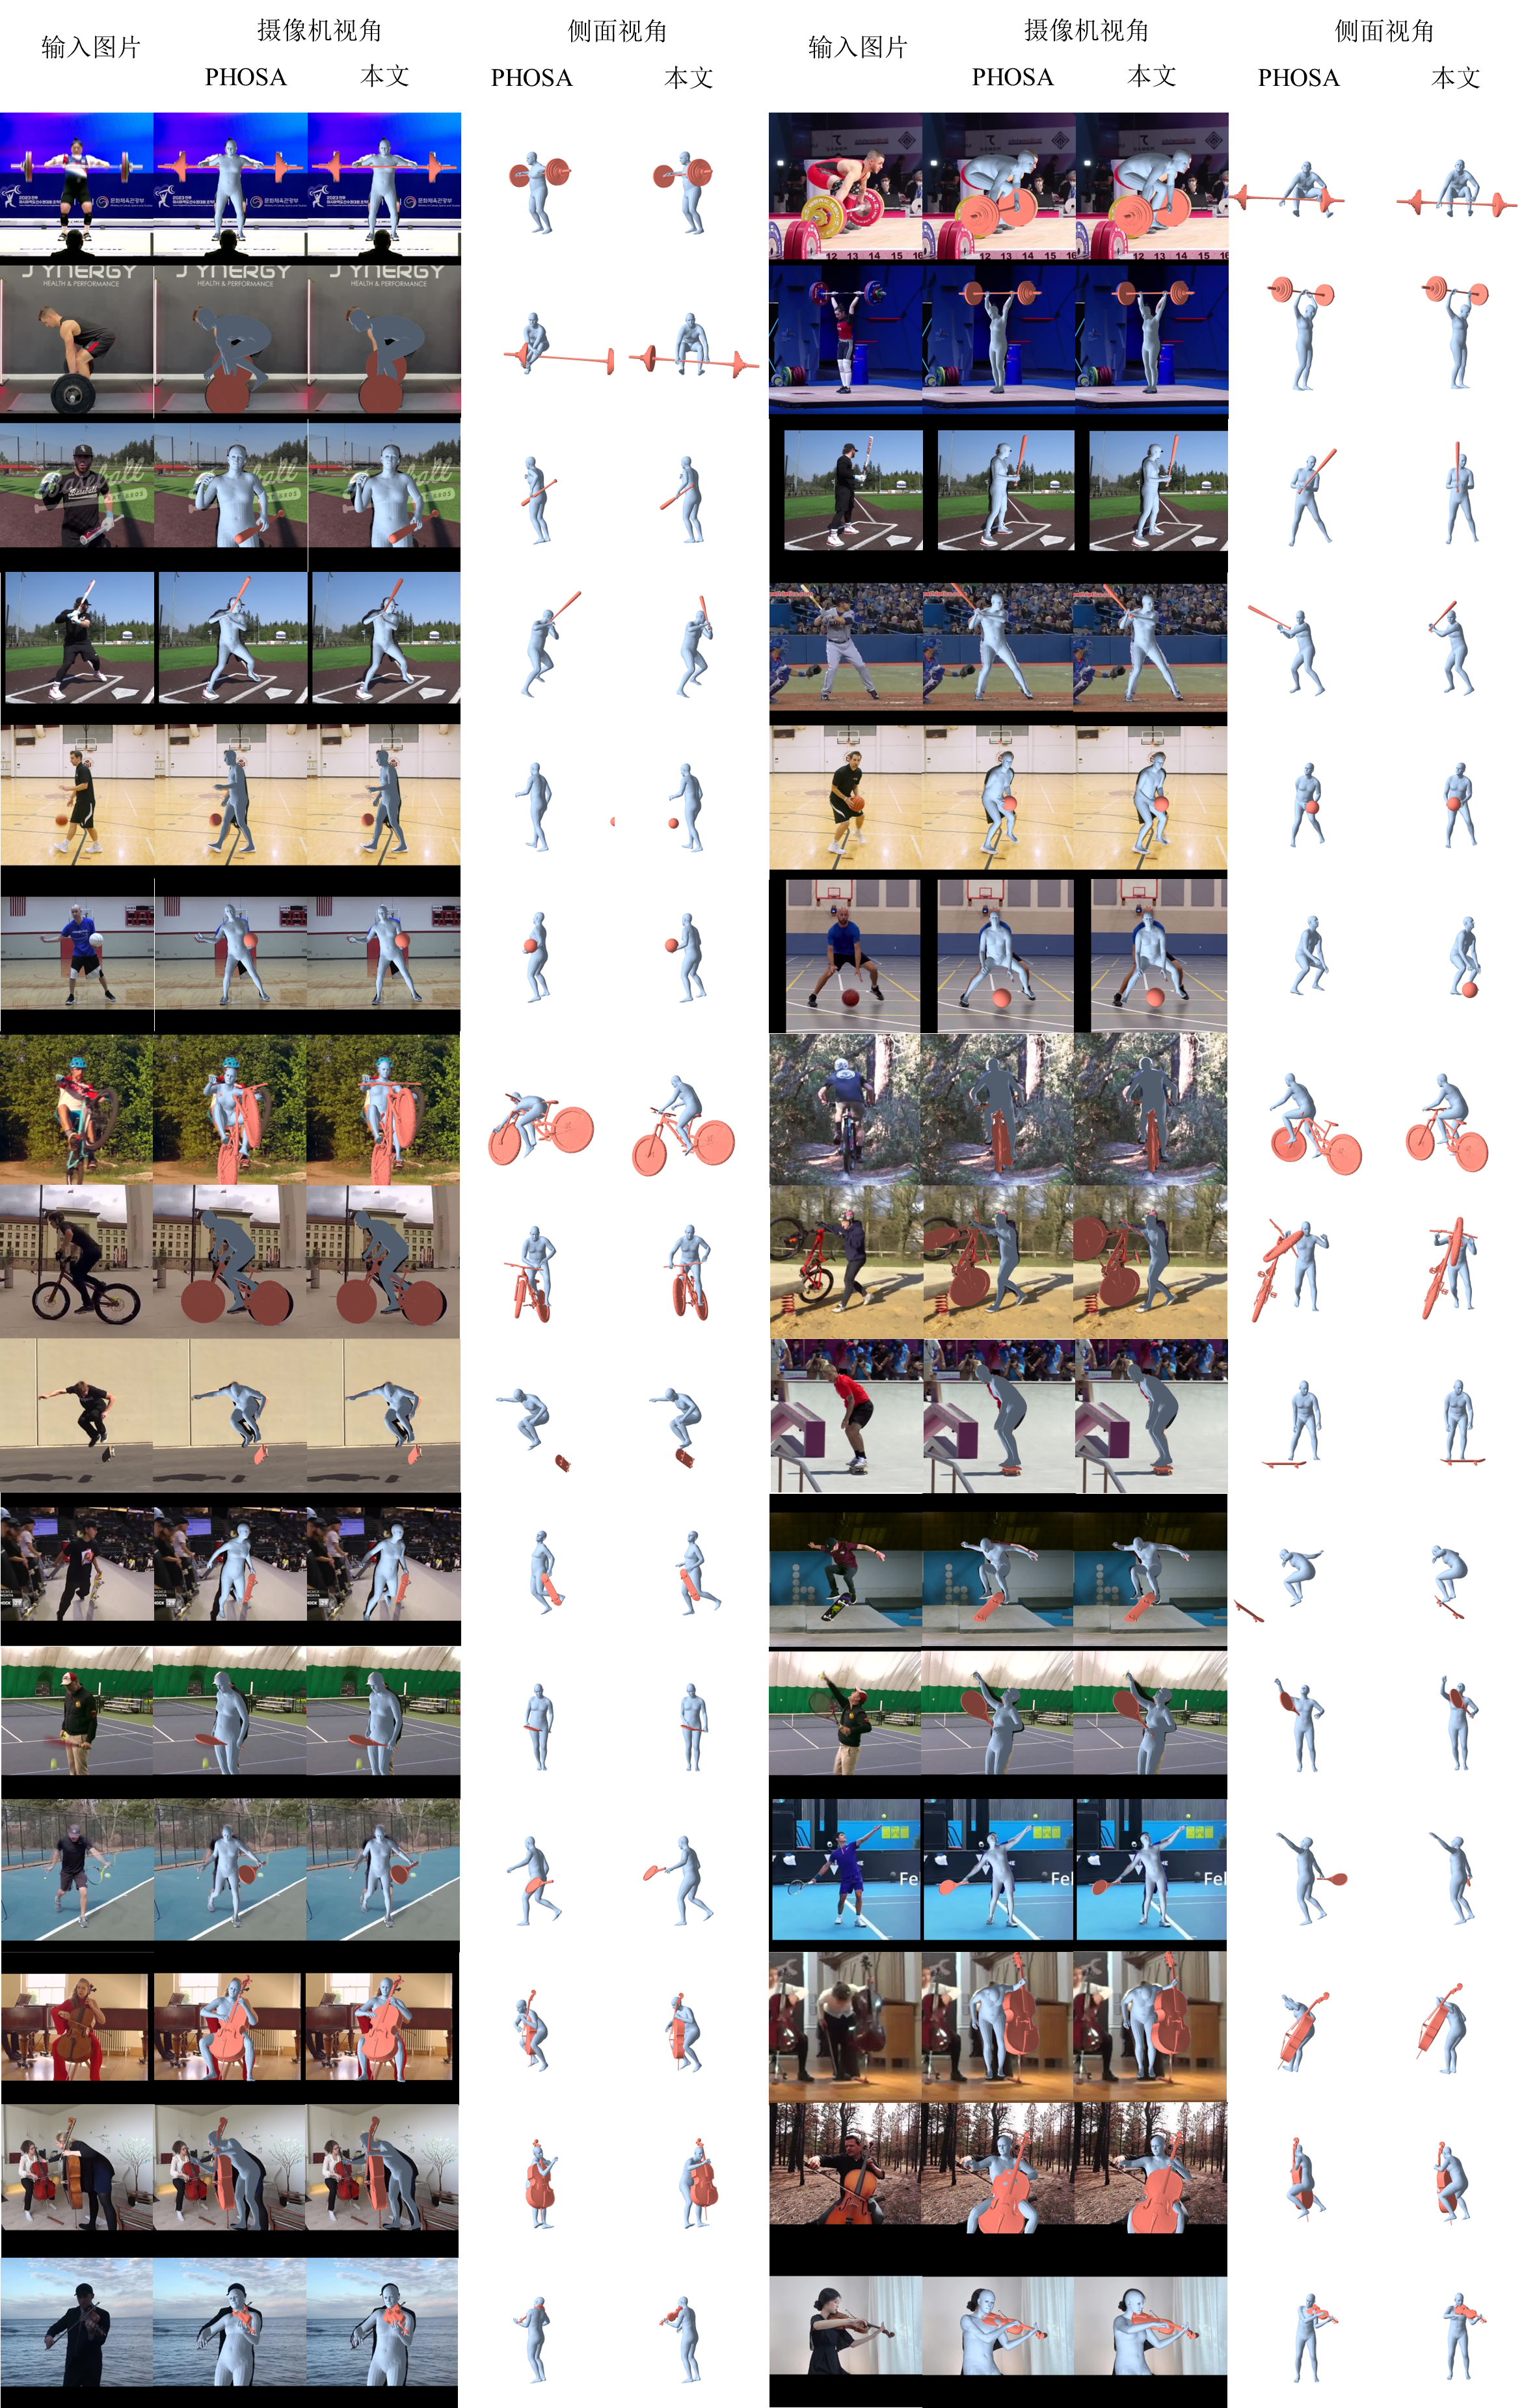
\includegraphics{Img/comparison_2d}
	\bicaption{本章所提出的方法和PHOSA在WildHOI数据集上的定性对比。}{Quantization comparison between our method and PHOSA on WildHOI dataset.}
	\label{fig:comparison-with-phosa}
\end{figure}

% \begin{figure}[!htbp]
% 	\centering
% 	\includegraphics[width=\linewidth]{Img/qualitative_results_sup_2}
% 	\bicaption{本章所提出的方法和PHOSA在WildHOI数据集上的定性对比。}{Quantization comparison between our method and PHOSA on WildHOI dataset.}
% 	\label{fig:comparison-with-phosa2}
% \end{figure}

\begin{figure}[!htbp]
	\centering
	\includegraphics[width=\linewidth]{Img/qualitative_results_sup_3}
	\bicaption{本章所提出的方法和PHOSA在WildHOI数据集上的定性对比。}{Quantization comparison between our method and PHOSA on WildHOI dataset.}
	\label{fig:comparison-with-phosa3}
\end{figure}

\begin{figure}[!htbp]
	\centering
	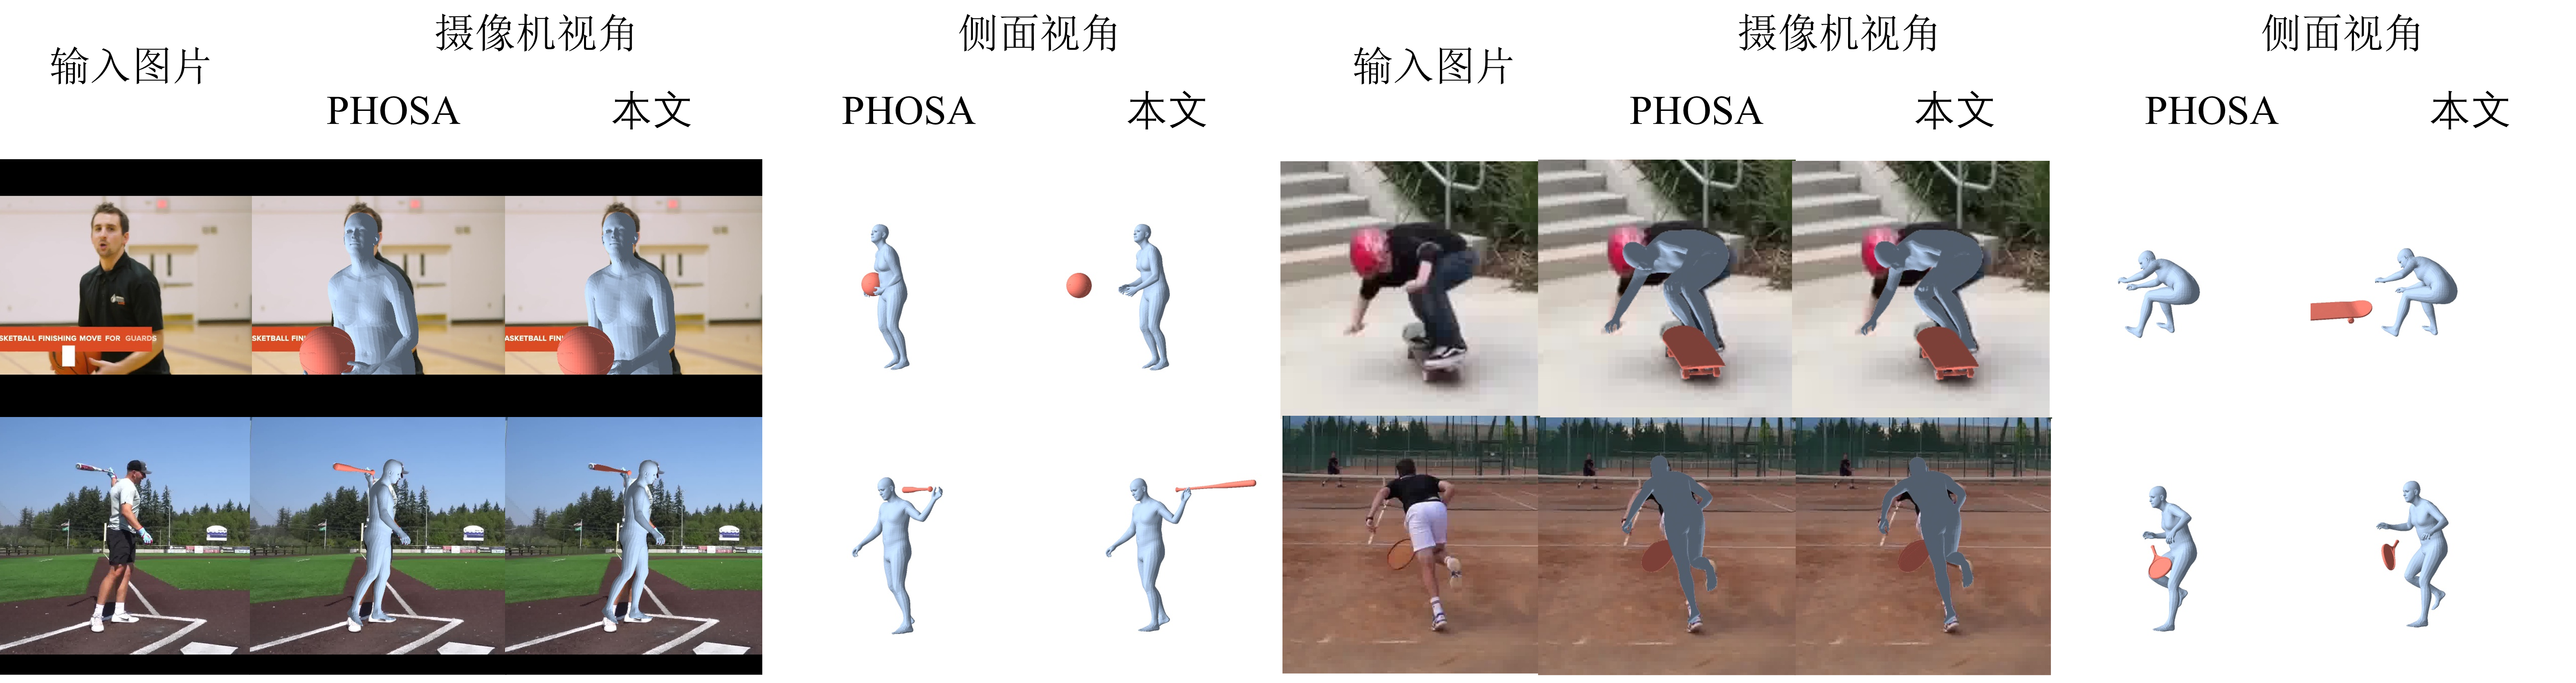
\includegraphics[width=0.9\linewidth]{Img/failures_2}
	\bicaption{在WildHOI-test数据集上的失败样例。}{Failures on WildHOI-test dataset.}
	\label{fig:failures}
\end{figure}

\paragraph{接触面损失和多视角二维关键点损失的有效性}
在表\ref{tab:ablation_contact_loss}中展示了对不同优化损失进行消融实验的结果。从实验结果可以看出,引入先验损失和接触面损失会带来最佳性能,除了在SMPL的倒角距离外,它在所有指标中达到最低的重建误差,这表明先验损失和接触面损失在优化过程发挥着重要作用。通过比较第三行和最后一行,可以看到去掉先验损失会导致重建准确度显著下降,这表明先验损失对重建精度有着更重要的影响。

\begin{table}[!htbp]
	\bicaption{\centering{不同损失对重建结果的影响。}}{\centering{The effectiveness of different losses on the reconstruction accuracy.}}
	\label{tab:ablation_contact_loss}
	\centering
	\footnotesize
	\setlength{\tabcolsep}{4pt}
	\renewcommand{\arraystretch}{1.2}
	\begin{tabular}{cccccc}
		\toprule
		$\mathcal{L}_{\text{prior}}$ & $\mathcal{L}_{\text{contact}}$ & SMPL (cm) $\downarrow$ & Obj. (cm) $\downarrow$ & Rot.($^\circ$) $\downarrow$ & Transl.(cm) $\downarrow$ \\
		\hline
		\XSolidBrush & \XSolidBrush & \textbf{3.57} & 1259.57 & 7.12 & 658.16 \\
		\XSolidBrush & \Checkmark & 3.71 & 363.40 & 6.47 & 195.62 \\
		\Checkmark & \XSolidBrush & 4.36 & 19.37 & 10.26 & 14.26 \\
		\Checkmark & \Checkmark & 4.43 & \textbf{17.48} & \textbf{10.12} & \textbf{13.13} \\
		\bottomrule
		\multicolumn{5}{l}{注:加粗字体为最优结果。}
	\end{tabular}
\end{table}

\paragraph{训练集规模对重建结果的影响} 在表\ref{tab:size_of_training_set}中比较使用不同规模的数据集训练的模型对重建结果的影响,越大的训练集可以带来更准确的重建结果,但微弱的指标提升表明训练集大小并不是影响模型重建精度的主要因素。

\begin{table}[!htbp]
	\bicaption{\centering{训练集大小对重建结果的影响。}}{\centering{The effectiveness of the size of training set on the reconstruction accuracy.}}
	\label{tab:size_of_training_set}
	\centering
	\footnotesize
	\setlength{\tabcolsep}{4pt}
	\renewcommand{\arraystretch}{1.2}
	\begin{tabular}{cccccc}
		\toprule
		训练集 & 测试集 & SMPL (cm) $\downarrow$ & Obj. (cm) $\downarrow$ & Rot.($^\circ$) $\downarrow$ & Transl.(cm) $\downarrow$ \\
		\hline
		50\% & 0\% & 4.48 & 18.53 & 10.41 & 13.76 \\
		75\% & 0\% & 4.31 & 18.15 & 10.35 & 13.33 \\
		100\% & 0\% & 4.43 & 17.48 & 10.12 & 13.13 \\
		100\% & 100\% & 4.34 & 18.07 & 10.40 & 13.44 \\
		\bottomrule
	\end{tabular}
\end{table}

\section{本章小结}
在本章中,探讨了如何从自然场景的二维图像中学习人和物体之间的空间关系的强先验。通过大量实验,展示了即使在不使用任何三维标注或者人体和物体之间三维空间关系的常识的前提下,本章所提出的方法可以在室内实验室场景下构建BEHAVE数据集和室外场景的WildHOI数据集上取得很好的结果。然而,本章所提出的工作仍然存在一些局限性。首先,该方法假设物体的形状是已知的,只聚焦于学习人体和物体的三维空间关系先验。这在物体形状变化很大的真实场景中并不太实用。此外,该方法严重依赖于大量的二维标注数据,而大规模的二维图片数据集并不是容易获得或者这种监督方式并不适用于所有任务。最后,该方法学习的是实例级别的先验而不是类别级先验,这可能对影响到对未见或稀有物体的泛化能力。

未来的研究方向可以包括以下几个方面的改进:
\begin{enumerate}
	\item 考虑物体形状的不确定性:可以引入形状建模和几何推理的方法,以适应不同形状的物体,并进一步提高模型的泛化能力。
	\item 减少对大量二维标注数据的依赖:可以探索使用弱监督或无监督学习的方法,减少对大量标注数据的需求,提高模型的数据利用效率。
	\item 学习类别级的空间关系先验:可以尝试引入类别信息,学习不同物体类别之间的空间关系先验,提高模型对不同类别的泛化能力。
\end{enumerate}

通过进一步探索和改进,可以使该方法在更广泛的应用场景中取得更好的效果,并为实际场景中的人体与物体关系推理提供更有效的解决方案。
\chapter{总结与展望}\label{chap:summary}

\section{全文总结}
本文围绕单视角人-物重建任务展开,针对人-物空间关系建模与预测、对未曾见过的物体的域外泛化、自然场景中人-物重建三方面提出了算法,有效的解决了单视角人-物空间关系中存在的挑战。

首先,在人-物空间关系建模与预测方面,提出了基于人-物偏移量的表征方式,使用人体和物体网格模型表面锚点之间的偏移量来刻画人体和物体之间的相对空间关系,并使用主成分降维的方式构造人-物空间关系的隐式空间。接着使用叠层归一化流模型从给定的图片中提取该空间关系的隐式表达,在后优化过程中,通过人-物偏移量损失和人-物重投影损失微调结果,实验中和先前方法在BEHAVE数据集和InterCap数据集进行了对比,本章所提出的算法在人-物重建方面取得了更高的重建精度和运行效率。

其次,针对未曾见过物体的域外泛化问题,传统基于学习的方法往往只能应用于训练集中见过的物体,无法很好地泛化到和新的形状物体交互上。为了应用该挑战,提出使用物体形状归一化模型将物体的形状映射到统一化的形状空间中,建立在该形状空间中人与物体之间的交互,测试时,那些未曾见过的物体被映射到该形状空间中,具有统一的表达,在训练集中的交互先验通过该形状空间迁移到新的物体上。实验中在CHAIRS数据集上和基于物体RT位姿的方法进行了比较,本章方法具有更好的泛化性能和交互迁移能力。

最后,在自然场景中人-物重建方面,由于自然场景中物体种类和交互类型的多样化,基于学习的方法受到数据集的限制不能应对多样性高的自然场景。为了解决这一问题,提出了一种二维监督的方法从大规模的二维数据中学习三维的人物空间交互先验知识的方法,该方法从二维图片中学习人-物交互的视角分布及其在各个视角下人-物二维关键点的分布,为了训练该网络,使用最近邻算法根据图片之间关键点的集合一致性对图片进行聚类以得到同一交互类型在其它视角下的二维关键点的分布情况。为了验证该算法,构造了自然场景中的数据集WildHOI,该数据集包含丰富的人和8个不同物体在各种场景中和不同物体之间的丰富的交互类型。实验中,在BEHAVE数据集和三维监督方法进行了对比,结果表明,本章所提出的方法即使没有直接使用三维标签监督训练网络也能够达到和三维监督方法近乎相媲美的性能,除室内BEHAVE数据集,还在自然场景的WildHOI数据集进行定性和定量实验,结果表明,本文所提出的方法相较于之前的方法对自然场景更加鲁棒,能够在不借助任何三维人-物相对空间关系的标注以及任何人和物体交互先验知识的前提下重建出合理的人和物体空间关系。

综上所述,本文提出的算法在单视角重建任务中取得了显著效果,为人-物交互关系建模和预测、对未曾见过物体的域外泛化、自然场景中人-物重建等问题提供了新的思路和方法。相信在不久的将来,三维空间中人-物交互将会取得更大的突破和进展,希望本文的研究能够为相关领域的研究工作提供一些有益的启示和参考。

\section{未来展望}

尽管本文所提出的算法在解决单视角人-物重建任务中取得较好效果,但仍然存在一些可以进行进一步改进和完善的方向:
\begin{enumerate}
	\item 首先,在人-物空间关系建模与预测方面,可以探索更灵活和有效的表征方式,例如结合局部和全局信息的表示学习方法,以提高人-物空间关系的建模和预测性能。另外,可以尝试结合目标检测和姿态估计等任务的信息,提升对人体和物体之间关系的理解和预测准确性。
	\item 其次,在对未曾见过的物体的域外泛化问题上,可以考虑引入更多的先验知识,例如利用物体的属性信息、材质信息等,提高模型的泛化能力和交互迁移效果。另外,可以探索使用生成对抗网络等方法进行形状归一化和统一化,以提高对未知物体的重建性能。
	\item 最后,在自然场景中人-物重建方面,可以加强对不同场景和不同交互类型的建模和预测能力,例如引入场景语义分割信息、场景布局信息等,提高模型对自然场景中人-物空间关系的理解和重建效果。同时,可以结合强化学习等方法,提高模型在复杂场景下的迁移和泛化能力,进一步提升人-物重建的性能。
\end{enumerate}

未来可以在改进现有算法的基础上,进一步探索和研究更加高效和稳健的方法,推动相关领域的研究工作取得更大的突破和进展。

\makebiblio

\backmatter
\begin{acknowledgement}
在论文写作过程中,得到了许多人的帮助和支持,我在此要向他们表示由衷的感谢。首先,我要感谢我的导师汪婧雅教授,在整个研究过程中给予我耐心的指导和宝贵的建议,让我能够顺利完成毕业论文的撰写。

再次,我要感谢实验室的老师和同学们,他们在我遇到困难时给予了无私的帮助和支持,让我能够顺利完成实验和数据分析。同时,我也要感谢论文评阅老师和答辩委员会的专家们,他们的审阅和指导使我对自己的研究有了更深刻的认识。

最后,我要感谢我的家人和朋友们,在我研究生期间给予了我精神上的支持和鼓励,让我能够坚持下来并顺利完成学业。他们的陪伴和支持是我前进的动力和力量。

再次谨向以上所有给予我支持和帮助的人表示由衷的感谢!没有你们的支持,我的论文也不可能如此顺利完成。希望以后继续保持联系,共同进步!
\end{acknowledgement}

\ifgraduate
\begin{resume}
    \paragraph{姓名:} 霍超凡。
    \paragraph{教育经历:}
    \begin{itemize}
        \item 2017年-2021年,本科就读于山东大学的软件工程专业,获得学士学位。
        \item 2021年-2024年,硕士就读于上海科技大学的计算机科学与技术专业,获得硕士学位。
    \end{itemize}

    \paragraph{研究方向:}
    \begin{itemize}
        \item 2021年-2024年,三维空间中人和物体交互重建。
        \item 2024年-?,三维场景重建与编辑。
    \end{itemize}
    \paragraph{联系方式:}
    \begin{description}
        \item[电子邮箱:] huochf@shanghaitech.edu.cn
        \item[联系电话:] 18633656293
    \end{description}
\end{resume}

\begin{publications}
  \begin{description}
    \item[(已发表)] [一作] \textbf{Chaofan Huo}, Ye Shi, Yuexin Ma, Lan Xu, Jingyi Yu, Jingya Wang. StackFLOW: Monocular Human-Object Reconstruction by Stacked Normalizing Flow with Offset. In Proceedings of the Thirty-Second International Joint Conference on Artificial Intelligence, {IJCAI-23}.
    \item[(已投递)] [一作] \textbf{Chaofan Huo}, Ye Shi, Jingya Wang. Monocular Human-Object Reconstruction in the Wild. In ACM MultiMedia 2024.
  \end{description}
\end{publications}

\begin{publications*}
  \begin{description}
    \item[(已发表)] [一作] ***, ***, ***, ***, ***. ***. In Proceedings of the Thirty-Second International Joint Conference on Artificial Intelligence, {IJCAI-23}.
    \item[(已投递)] [一作] ***, ***, ***. ***. In ACM MultiMedia 2024.
  \end{description}
\end{publications*}

% \begin{patents}
%   专利申请或授权记录…… (非匿名环境)
% \end{patents}

% \begin{patents*}
%   专利申请或授权记录…… (匿名环境)
% \end{patents*}

% \begin{projects}
%   个人参与的科研项目、获奖情况…… (仅非匿名环境显示)
% \end{projects}
\fi

\end{document}
